\documentclass[letter, 12pt]{report}

%%%%%%%%%%%%%%%%%%%%%%%%%%%%%%%%%%%%%%%%%%%%%%%%%%%%%%%%%%%%%%%%%%%%%%%%%%%
%%%%%%%%%%%%%%%%%%%%%%%%%%%%%%%%%%%%%%%%%%%%%%%%%%%%%%%%%%%%%%%%%%%%%%%%%%%
%%%%%%%%%%%%%%%%%%%%%%%%%%%%%    packages    %%%%%%%%%%%%%%%%%%%%%%%%%%%%%%
%%%%%%%%%%%%%%%%%%%%%%%%%%%%%%%%%%%%%%%%%%%%%%%%%%%%%%%%%%%%%%%%%%%%%%%%%%%
%%%%%%%%%%%%%%%%%%%%%%%%%%%%%%%%%%%%%%%%%%%%%%%%%%%%%%%%%%%%%%%%%%%%%%%%%%%
\usepackage[utf8]{inputenc}
\usepackage[USenglish]{babel}
\usepackage{colorprofiles}
\usepackage[a-3b,mathxmp]{pdfx}[2018/12/22]
\usepackage{fullpage}
\usepackage{titling}
\usepackage{nicefrac}
\usepackage{xcolor}
\usepackage{amsmath}
\usepackage{amssymb}
\usepackage{amsthm}
\usepackage{hyperref}
\usepackage{bbm}
\usepackage{lineno}
\usepackage{multirow}
\usepackage{longtable}
\usepackage{makecell}
\usepackage{lipsum}
\usepackage{etoolbox} %% <- for \pretocmd and \apptocmd
\usepackage[noend]{algpseudocode}
\usepackage[normalem]{ulem}
\usepackage{thmtools, thm-restate}
\usepackage[nottoc]{tocbibind} % for adding list of figures to the table of contents
% packages from colt
\usepackage{comment}
\usepackage{listings}
\lstset{emph={try,catch,throw,def,or,to,for,then,end,for,if,args,else,return},emphstyle=\color{blue!100!black}\textbf}
\lstset{mathescape=true,escapechar=\&,numbers=left,xleftmargin=3mm,linewidth=0.47\textwidth,framextopmargin=0pt,framexbottommargin=0pt,aboveskip=-1pt,belowskip=-1pt}
\usepackage{mdframed}
\mdfsetup{skipabove=0pt,skipbelow=0pt,backgroundcolor=black!3}
\usepackage{pgfplots}
\pgfplotsset{compat=1.17}
\usepackage{tikz}
\usetikzlibrary{3d}
\usetikzlibrary{arrows.meta,calc,positioning,shapes.callouts}
\setlength{\marginparwidth}{2cm}
\usepackage[colorinlistoftodos,prependcaption,textsize=tiny,disable]{todonotes}
\newcommand{\todoc}[2][]{\todo[size=\scriptsize,color=blue!20!white,#1]{Csb: #2}}
\newcommand{\todoa}[2][]{\todo[size=\scriptsize,color=green!20!white,#1]{Alr: #2}}
\definecolor{dkblue}{cmyk}{1,.54,.04,.19}
\usepackage{enumitem}
\usepackage{times}
\pgfplotsset{compat=1.11}
\usepackage{pgfplotstable}
\usepackage{multicol}
\usepackage{colortbl}
\usepackage{floatrow}
\usepackage{setspace}
\usepackage{mathtools}
\usepackage{mathrsfs}
\usepackage{soul}
\usepackage{wrapfig}
\usepackage{dsfont}
\usepackage[plain]{algorithm}
\usepackage{bm}
\usepackage[bf]{caption}
\usepackage{graphicx}
\usepackage{subcaption}
\usepackage[capitalize]{cleveref}
\usepackage{natbib}
\hypersetup{
    pdfstartview=,
    colorlinks,
    linkcolor={red!33!black},
    citecolor={blue!33!black},
    urlcolor={blue!33!black}
}
\setlength{\droptitle}{-6em}   % This is your set screw, for shifting up the title
\setlength{\parskip}{0.5em} % paragraph spacing
\usepackage{xspace}
\usepackage{placeins}
%%%%%%%%%%%%%%%%%%%%%%%%%%%%%%%%%%%%%%%%%%%%%%%%%%%%%%%%%%%%%%%%%%%%%%%%%%%
%%%%%%%%%%%%%%%%%%%%%%%%%%%%%%%%%%%%%%%%%%%%%%%%%%%%%%%%%%%%%%%%%%%%%%%%%%%
%%%%%%%%%%%%%%%%%%%%%%%%%%%%%    commands    %%%%%%%%%%%%%%%%%%%%%%%%%%%%%%
%%%%%%%%%%%%%%%%%%%%%%%%%%%%%%%%%%%%%%%%%%%%%%%%%%%%%%%%%%%%%%%%%%%%%%%%%%%
%%%%%%%%%%%%%%%%%%%%%%%%%%%%%%%%%%%%%%%%%%%%%%%%%%%%%%%%%%%%%%%%%%%%%%%%%%%
\renewcommand{\baselinestretch}{1.1} % line spacing
\newcommand{\epsF}{{\epsilon_{\text{\tiny \textsc{f}}}}}
\newcommand{\epsR}{{\epsilon_R}}
\newcommand{\epsO}{{\epsilon_O}}
\newcommand{\opt}{\operatorname{\textsc{optr}}}
\newcommand{\opte}{\operatorname{\textsc{opt}}}
\newcommand{\hopt}{\operatorname{\widetilde{\textsc{optr}}}}
\newcommand{\pr}{\text{\tiny\texttt{r}}}
\newcommand{\pb}{\text{\tiny\texttt{b}}}
\newcommand{\pl}{\text{\tiny\texttt{l}}}
\renewcommand{\pm}{\text{\tiny\texttt{m}}}
\newcommand{\ceil}[1]{\left\lceil #1 \right\rceil}
\newcommand{\floor}[1]{\left\lfloor #1 \right\rfloor}
\newcommand{\pair}{\operatorname{\textsc{pair}}}
\newcommand{\spt}{\operatorname{spt}}
\newcommand{\R}{\mathbb R}
\newcommand{\bR}{\mathbb R}
\newcommand{\bN}{\mathbb N}
\newcommand{\eye}{\mathbf{1}}
\newcommand{\esssup}{\operatorname{ess\,sup}}
\newcommand{\essinf}{\operatorname{ess\,inf}}
\newcommand{\argmin}{\operatornamewithlimits{arg\,min}}
\newcommand{\argmax}{\operatornamewithlimits{arg\,max}}
\newcommand{\explan}[1]{\stackrel{\text{\tiny \texttt{#1}}}}
\newcommand{\ip}[1]{\left \langle #1 \right \rangle}
\newcommand{\bip}[1]{\left\langle #1 \right\rangle}
\newcommand{\sip}[1]{\langle #1 \rangle}
\newcommand{\Reg}{\textup{\textrm{Reg}}}
\newcommand{\esup}{\operatorname{ess\,sup}}
\newcommand{\uReg}{\overline{\textrm{Reg}}}
\newcommand{\BReg}{\textrm{BReg}}
\newcommand{\Breg}{\operatorname{D}}
\newcommand{\Fmax}{\textup{\textrm{F}}_{\max}}
\newcommand{\Hmax}{\textrm{H}_{\max}}
\newcommand{\Bmax}{\textrm{B}_{\max}}
\newcommand{\Rmax}{\textrm{R}_{\max}}
\newcommand{\Rmin}{\textrm{R}_{\min}}
\newcommand{\Kmax}{\textrm{K}_{\max}}
\newcommand{\sphere}{\mathbb{S}}
\newcommand{\logs}{L}
\newcommand{\KL}{\operatorname{KL}}
\newcommand{\ball}{\mathbb{B}}
\newcommand{\paren}[1]{\left( #1 \right)}
\newcommand{\abs}[1]{\left| #1 \right|}
\newcommand{\brak}[1]{\left[ #1 \right]}
\newcommand{\sett}[1]{\left\{ #1 \right\}}
\newcommand{\norm}[1]{\left \Vert  #1 \right \Vert}
\newcommand{\snorm}[1]{ \Vert  #1 \Vert}
\newcommand{\Lsnorm}[1]{ \Vert  #1 \Vert_{\text{\scriptsize \textrm{L}$^2$}}}
\newcommand{\sS}{\mathscr S}
\newcommand\half[1]{\textstyle{\frac{#1}{2}}}
\newcommand{\ext}{\operatorname{e}}
\newcommand{\psd}{\mathbb S^+}
\newcommand{\cond}{\operatorname{cond}}
\newcommand{\normt}[2]{\Vert #2 \Vert_{#1}}
\newcommand{\bnorm}[1]{\left\Vert #1 \right\Vert}
\newcommand{\barnorm}[1]{\bar \Vert #1 \bar \Vert}
\newcommand{\bignorm}[1]{\bigl\Vert #1 \bigr\Vert}
\newcommand{\E}{\mathbb E}
\newcommand{\EE}{\mathbb E}
\newcommand{\T}{\top}
\newcommand{\grad}{\nabla}
\newcommand{\Var}{\mathbb V}
\newcommand{\err}[1]{\operatorname{err}_{\ref{#1}}}
\newcommand{\cE}{\mathcal E}
\newcommand{\Cnst}{\textrm{C}}
\newcommand{\cnst}{\textrm{c}}
\newcommand{\cK}{\mathcal K}
\newcommand{\cH}{\mathcal H}
\newcommand{\cF}{\mathcal F}
\newcommand{\cC}{\mathcal C}
\newcommand{\cT}{\mathcal T}
\newcommand{\sG}{\mathscr G}
\newcommand{\sF}{\mathscr F}
\newcommand{\cL}{\mathcal L}
\newcommand{\cI}{\mathcal I}
\newcommand{\cS}{\mathcal S}
\newcommand{\cD}{\mathcal D}
\newcommand{\cP}{\mathcal P}
\newcommand{\cO}{\mathcal O}
\newcommand{\Z}{\mathbb Z}
\newcommand{\cN}{\mathcal N}
\newcommand{\cM}{\mathcal M}
\newcommand{\sB}{\mathscr B}
\newcommand{\sA}{\mathscr A}
\newcommand{\sP}{\mathscr P}
\newcommand{\cX}{\mathcal X}
\newcommand{\bS}{\mathbb S}
\newcommand{\bB}{\mathbb B}
\newcommand{\tr}{\operatorname{tr}}
\newcommand{\cHb}{\mathcal H_{\circ}}
\newcommand{\zeros}{ \bm 0}
\newcommand{\ones}{ \bm 1}
\newcommand{\bbP}{\mathbb P}
\newcommand{\N}{\mathbb N}
\newcommand{\lip}{\operatorname{Lip}}
\newcommand{\vol}{\operatorname{vol}}
\newcommand{\polylog}{\operatorname{polylog}}
\newcommand{\const}{\operatorname{const}}
\newcommand{\interior}{\operatorname{int}}
\newcommand{\conv}{\operatorname{conv}}
\newcommand{\diam}{\operatorname{diam}}
\newcommand{\poly}{\operatorname{poly}}
\newcommand{\sind}{\bm{1}}
\renewcommand{\d}[1]{\operatorname{d}\!#1}
\newcommand{\id}{\mathds{1}}
\newcommand{\I}{\mathcal{I}}
\newcommand{\1}{\mathbf{1}}
\newcommand{\cY}{\mathcal{Y}}
\newcommand{\mP}{\mathbb{P}}
\newcommand{\mI}{\mathbb{I}}
\newcommand{\IR}{\operatorname{\textsc{ir}}}
\newcommand{\bco}{\texttt{BCO}\xspace}
\newcommand{\ts}{\textsc{TS}\xspace}
\newcommand{\ats}{\textsc{ATS}}
\newcommand{\IDS}{\textsc{IDS}}
% Math/algorithm helpers
\newcommand{\prop}{\mathrm{prop}}
\newcommand{\Normal}{\mathcal{N}}
\newcommand{\diag}{\mathrm{diag}}
\newcommand{\ESS}{\textsc{ESS}}
\newcommand{\rdec}{\text{dec}}
\newcommand{\dec}{\text{dec}}
\newcommand{\acpacdec}{\text{{\normalfont pac-dec}}^{ac}}
\newcommand{\acfpacdec}{\text{{\normalfont pac-dec}}^{ac,f}}
\newcommand{\acdec}{\text{{\normalfont dec}}^{ac}}
\newcommand{\acfdec}{\text{{\normalfont dec}}^{ac,f}}
\newcommand{\odec}{\text{{\normalfont dec}}^{o}}
\newcommand{\cdec}{\text{{\normalfont dec}}^{c}}
\newcommand{\dc}{\text{{\normalfont dc}}}
\newcommand{\sthat}{\qquad\text{s.t.}\qquad}
\newcommand{\eps}{\epsilon}
\newcommand{\AETD}{\textsc{Anytime-E2D}}
\newcommand{\ETD}{\textsc{E2D}}
\newcommand{\UCB}{\textsc{UCB}}
\newcommand{\TSa}{\textsc{TS}}
\newcommand{\ETDp}{\textsc{E2D$^+$}}
\newcommand{\Est}{\text{{\normalfont Est}}}
\newcommand{\EST}{\text{{\normalfont EST}}}
\newcommand{\co}{\text{{\normalfont co}}}
\DeclareMathOperator{\Log}{Log}
\renewcommand{\epsilon}{\varepsilon}
%%%%%%%%%%%%%%%%%%%%%%%%%%%%%%%%%%%%%%%%%%%%%%%%%%%%%%%%%%%%%%%%%%%%%%%%%%%
%%%%%%%%%%%%%%%%%%%%%%%%%%%%%%%%%%%%%%%%%%%%%%%%%%%%%%%%%%%%%%%%%%%%%%%%%%%
%%%%%%%%%%%%%%%%%%%%%%%%%%%%%     stuff      %%%%%%%%%%%%%%%%%%%%%%%%%%%%%%
%%%%%%%%%%%%%%%%%%%%%%%%%%%%%%%%%%%%%%%%%%%%%%%%%%%%%%%%%%%%%%%%%%%%%%%%%%%
%%%%%%%%%%%%%%%%%%%%%%%%%%%%%%%%%%%%%%%%%%%%%%%%%%%%%%%%%%%%%%%%%%%%%%%%%%%
\theoremstyle{plain}
\newtheorem{theorem}{Theorem}
% \newtheorem{example}[theorem]{Example}
\newtheorem{optprob}[theorem]{optimization Problem}
\newtheorem{lemma}[theorem]{Lemma}
\newtheorem{proposition}[theorem]{Proposition}
\newtheorem{corollary}[theorem]{Corollary}
\newtheorem{claim}[theorem]{Claim}
\theoremstyle{definition}
\newtheorem{definition}[theorem]{Definition}
\newtheorem{assumption}[theorem]{Assumption}
\newtheorem{example}[theorem]{Example}
\newtheorem{remark}[theorem]{Remark}
\theoremstyle{remark}
\setlist[itemize,1]{label={$\circ$},itemsep=0pt,labelindent=0pt,labelwidth=!,leftmargin=14pt}
\newlist{enumroman}{enumerate}{1}
\newlist{enumsteps}{enumerate}{1}
\newlist{enumcases}{enumerate}{1}
\setlist[enumcases,1]{label={\normalfont\sffamily\textbf{\textsc{\color{dkblue}case \arabic*}}},itemsep=0pt,wide,labelwidth=!,labelindent=0pt,itemsep=0pt}
\setlist[enumerate,1]{label={\normalfont\texttt{(\alph*)}},itemsep=0pt,wide,labelwidth=!,labelindent=0pt,itemsep=0pt}
\setlist[enumroman,1]{label={\normalfont\texttt{\color{dkblue}(\uline{\roman*})}},itemsep=0pt,wide,labelwidth=!,labelindent=0pt,itemsep=0pt}
\setlist[enumsteps,1]{label={\normalfont\sffamily\textbf{\textsc{\color{dkblue}step \arabic*}}},itemsep=0pt,wide,labelwidth=!,labelindent=0pt,itemsep=0pt}
%\setlist[description]{itemsep=0pt,labelwidth=!,labelindent=0pt,wide,leftmargin=0pt}
\setlist[description]{itemsep=0pt,wide,labelwidth=!,labelindent=0pt,itemsep=0pt,format={\normalfont \textit}}
%%%%%%%%%%%%%%%%%%%%%%%%%%%%%%%%%%%%%%%%%%%%%%%%%%%%%%%%%%%%%%%%%%%%%%%%%%%
%%%%%%%%%%%%%%%%%%%%%%%%%%%%%%%%%%%%%%%%%%%%%%%%%%%%%%%%%%%%%%%%%%%%%%%%%%%
%%%%%%%%%%%%%%%%%%%%%%%%%%%%%    document    %%%%%%%%%%%%%%%%%%%%%%%%%%%%%%
%%%%%%%%%%%%%%%%%%%%%%%%%%%%%%%%%%%%%%%%%%%%%%%%%%%%%%%%%%%%%%%%%%%%%%%%%%%
%%%%%%%%%%%%%%%%%%%%%%%%%%%%%%%%%%%%%%%%%%%%%%%%%%%%%%%%%%%%%%%%%%%%%%%%%%%
\begin{document}

\setcounter{page}{1}
\renewcommand{\thepage}{\roman{page}} % Roman numerals for page counter

\begin{titlepage}
    \centering
    \textbf{\large{Thompson Sampling for Bandit Convex Optimization\\(Version 3.0)}}
    \vskip.5in by \vskip.5in
    \large{Alireza Bakhtiari}

    \vfill \vfill
    A thesis submitted in partial fulfillment of the requirements for the degree of
    \vskip.3in Master of Science
    \vskip.3in \vfill \vfill
    Department of Computing Science
    \vskip.3in
    University of Alberta
    \vfill \vfill
    $\copyright$ Alireza Bakhtiari, 2025
\end{titlepage}

\doublespacing

\chapter*{Abstract}
\addcontentsline{toc}{chapter}{Abstract}
Thompson sampling (\ts) is a popular and empirically successful algorithm for online decision-making problems.
This thesis advances our understanding of \ts when applied to bandit convex optimization (\bco) problems,
by providing new theoretical guarantees and characterizing its limitations.

First, we analyze $1$-dimensional \bco and show that \ts achieves a near-optimal Bayesian regret of at most $\tilde O(\sqrt{n})$, where $n$ is the time horizon.
This result holds without strong assumptions on the loss functions, requiring only convexity, boundedness, and a mild Lipschitz condition.
In sharp contrast, we demonstrate that for general high-dimensional problems, \ts can fail catastrophically.

More positively, we establish a Bayesian regret bound of $\tilde O(d^{2.5} \sqrt{n})$ for \ts in generalized linear bandits, even when the convex monotone link function is unknown.
Finally, we prove a fundamental limitation of current analysis techniques: we show that the standard information-theoretic machinery can never yield a regret bound better than the existing $\tilde O(d^{1.5} \sqrt{n})$ in the general case.

\setcounter{page}{2}
\renewcommand{\thepage}{\roman{page}} % Roman numerals for page counter

\onehalfspacing
\chapter*{Preface} \addcontentsline{toc}{chapter}{Preface}
The first part of this thesis has been published as Alireza Bakhtiari,
Tor Lattimore, and Csaba Szepesv\'ari.
Thompson Sampling for Bandit Convex Optimization.
In International Conference on Learning Theory, 2025.

\chapter*{Acknowledgements} \addcontentsline{toc}{chapter}{Acknowledgements}
I would like to sincerely thank my supervisor, Csaba,
for his time, mentorship, guidance, and patience throughout my studies.
Csaba gave me the opportunity to pursue what I love most and provided me with unconditional intellectual freedom.
His passion for research and honest approach to science have been a true inspiration.
I also extend my gratitude to Tor Lattimore for his time and for teaching me the ways of research; his insights have profoundly shaped my thinking.
Special thanks go to Dave Janz and Johannes Krishner for their close guidance and constructive feedback in shaping my research.
Moreover, I am deeply grateful to my labmates—listed
in alphabetical order as Alex prefers—Alex Ayoub, Kushagra Chandak,
Shuai Liu, Samuel Robertson, and Vlad Tkachuk, for patiently
listening to my ideas, providing valuable feedback,
and assisting me in my research.
This journey would have been far less enjoyable without
their presence.
I am also thankful to my friends for always being there when
needed, and to my partner, Zahra, for her unwavering patience,
support, and encouragement.
Lastly, I feel incredibly fortunate to have my parents, Pooneh and Majid, whose although been far away, have always kept their love and care present in my life, and my brother, Amin, whose presence makes my life much more colorful and vibrant.

\tableofcontents
\listoftables
\listoffigures
\listofalgorithms \addcontentsline{toc}{chapter}{List of Algorithms}

\clearpage
\setcounter{page}{1}   % Start at page 1
\renewcommand{\thepage}{\arabic{page}} % Roman numerals for page counter

% \part{Thompson Sampling for Bandit Convex Optimization}
\chapter{Introduction} \label{ch:intro}
In this chapter we introduce the bandit convex optimization (\bco) problem, and its relation to other related settings.
Convexity is a common assumption in optimization problems \citep{boyd2004convex}.
In convex optimization, the goal is to find the minimum of a convex function over a convex set, typically with access to the function's value and gradient at any point in the domain.
Formally, the objective is to approximately solve the optimization problem
\begin{align}
    \argmin_{x \in \cK} f(x)\,,
\end{align}
where \( \cK \subset \mathbb{R}^d \) is a convex set (typically compact with non-empty interior) and \( f : \cK \to \mathbb{R} \) is a convex function.
Broadly, convex optimization algorithms use function evaluations $f(x)$ as well as gradient and higher order information of $f$ to find the minimizer.

A related setting is the \emph{zeroth-order} optimization, where the learner (optimization algorithm) just gets access to function's evaluations for points $x\in\cK$, and no other information about $f$ like its gradient.
Precisely, for $n$ many rounds, the algorithm selects a point \( x_t \in \cK \) and receives feedback \( y_t = f(x_t)\) for $t \in \{1, \ldots, n\}$, and use these evaluations to find (approximate) the minimizer of $f$.

Compared to classical convex optimization and \emph{zeroth-order} optimization, the \bco problem is characterized by two key features:
\begin{enumroman}
    \item \textcolor{dkblue}{Limited Noisy Access:} The algorithm can only observe \textit{noisy} point evaluations of the objective function, i.e. the feedback is of the form \( f(x_t) + \epsilon_t \), where \( \epsilon_t \) is the noise.
    \item \textcolor{dkblue}{Cumulative Cost:} The goal is to minimize the cumulative cost of these evaluations over time, rather than to identify the function’s minimizer.
\end{enumroman}

\begin{wrapfigure}[14]{r}{0.48\textwidth} % [lines]{placement}{width}
    \vspace{-8pt}                           % pull figure up a bit (optional)
    \centering
    % If you compiled the standalone TikZ file to PDF:
    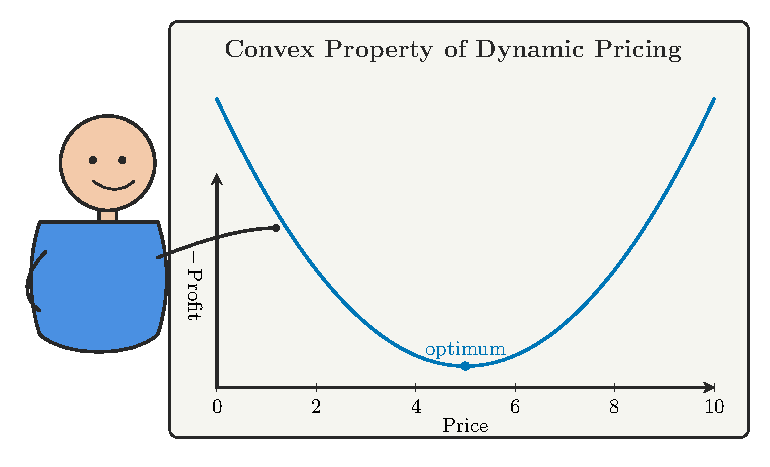
\includegraphics[width=\linewidth]{figures/dprice.pdf}
    % Or include the standalone TikZ source directly:
    %   \includestandalone[width=\linewidth]{convex_dynamic_pricing}
    \caption{Convex property of dynamic pricing (\(x=\) price, \(y=-\)profit).}
    \vspace{-6pt}                           % tighten space below (optional)
\end{wrapfigure}
A representative example of \bco is dynamic pricing, where a seller selects a price (the input) and observes the resulting negative-profit (the output), which is often modeled as a convex function of the price.
The seller cannot directly observe the profit function itself, but only noisy feedback through customer purchases at chosen prices. Each evaluation corresponds to a real transaction and thus incurs a potentially significant cost. In such cases, the objective is not to eventually find the best price at any expense, but rather to make pricing decisions that yield high cumulative profit over time.

Precisely, the learner in the \bco setting aims to minimize the cumulative loss over \( n \) rounds,
which leads to the online variant of the optimization problem.
The goal after $n$ rounds of interaction is to minimize the cumulative loss compared to the best fixed point in hindsight,
which is
\begin{align}
    \sum_{t=1}^n f(x_t) - \min_{x \in \cK} \sum_{t=1}^n f(x)\,,
\end{align}
referred to as \emph{regret}. This perspective connects \bco to the broader literature on online learning and multi-armed bandits. While \bco is challenging due to the simultaneous absence of gradient information and the need for exploration, it offers a powerful abstraction for decision-making under uncertainty with limited feedback.

\section{Examples of \bco}
\bco naturally arises in a variety of applications where gradient information is unavailable, unreliable, or too expensive to compute, and where each $f$ evaluation comes with a cost. Here are some examples:
\begin{description}
    % \item[\textcolor{dkblue}{Manufacturing:}]
    %       Consider a cheese factory that aims to optimize its recipe by adjusting the temperature and humidity of its warehouse.
    %       The negative quality of the final product can be modeled as a convex function of these parameters.
    %       However, each measurement becomes available only after the batch is complete, and producing a batch incurs a financial cost.
    %       The factory’s goal is to iteratively improve product quality based on customer feedback, but it cannot afford to ruin too many batches in the process.
    %       This situation is even more pronounced for expensive or custom products—like cars, airplanes, or musical instruments—where each failed experiment is prohibitively costly and feedback may only be available post-sale.

    \item[\textcolor{dkblue}{Hyperparameter Tuning:}]
          Optimizing hyperparameters is a challenge for systems that can only get evaluations of their performance through live deployment.
          For instance, consider an automated trading algorithm with tunable hyperparameters.
          Its performance—measured by profit—can often be modeled as a convex function of these parameters.
          Evaluating performance requires running the algorithm live, which comes with financial risk and opportunity cost.
          Since the system is deployed in production, the goal is not to identify the best hyperparameters in hindsight, but to continually adapt and improve performance over time with minimal cumulative loss.

    \item[\textcolor{dkblue}{Dynamic Pricing:}]
          In dynamic pricing, a retailer interacts sequentially with an uncertain market.
          At each round, they select a price \(X_t \in \cK \subset \R\), and the associated loss \(f(X_t)\) represents the negative of expected profit.
          Prices that are too high may deter purchases, while prices that are too low leave revenue on the table.
          The profit function \(f\) is unknown in advance and customer behavior introduces noise into observations.
          The goal is to adjust prices over time to maximize cumulative profit, not just to identify an optimal price after at any cost.

    \item[\textcolor{dkblue}{Service Personalization:}]
          Large Language Models (LLMs) often personalize their responses based on user preferences.
          At each interaction, the system selects a response style \(X_t \in \cK \subset \R^d\) — e.g., controlling tone, formality, or humor.
          The user’s satisfaction is captured by a loss function \(f(X_t)\), which reflects poor alignment with their preferences.
          This function is unknown, subjective, and observed only through noisy feedback such as click-through rates or engagement metrics.
          The system must learn and adapt over time to minimize dissatisfaction, making this a natural fit for the bandit convex optimization setting.

    \item[\textcolor{dkblue}{Resource Allocation:}]
          Many decision-making problems involve allocating limited resources—like budget or bandwidth—across competing options.
          For example, a company might distribute marketing funds across various channels.
          The return on investment typically exhibits diminishing returns and can be modeled by a convex utility function.
          The utility is not directly observable but can be estimated after committing to a specific allocation.
          Since each evaluation carries cost, the company seeks to minimize cumulative regret over time by carefully balancing exploration and exploitation.

    \item[\textcolor{dkblue}{Online Advertising---$\R$-valued parameters:}]
          Online advertisement is a classical application of bandit algorithms.
          Often, advertisers can choose among nearly-continuous design parameters—like font size and color.
          These decisions affect user engagement in a way that can be modeled by a convex function over the parameter space.
          The feedback (e.g., click-through rates) is noisy and delayed, and testing each variation has opportunity cost.
          Bandit convex optimization provides a principled framework to navigate this space efficiently and improve ad performance over time.

    \item[\textcolor{dkblue}{Efficiency Tuning:}]
          In commercial aviation, dispatchers must decide the cruise altitude and Mach number for each flight, represented as \(X_t = (\text{Mach}, \text{Altitude}) \in \cK \subset \R^2\).
          The loss \(f(X_t)\) is the fuel burned per seat-kilometre—a quantity well-approximated by a convex function due to the trade-offs between speed, altitude, and drag.
          Crucially, the true fuel burn is revealed only after the flight, and is confounded by weather, routing, and payload variability.
          Since each evaluation corresponds to a real flight with significant operational cost, the airline cannot afford extensive trial-and-error.
          Instead, it must adapt its cruise settings sequentially, improving fuel efficiency over time while minimizing total cost—an ideal use case for bandit convex optimization.
\end{description}



\chapter{Related work}
\bco in the regret setting was first studied by \cite{FK05} and \cite{Kle04}. Since then the field has grown considerably as summarized
in the recent monograph by \cite{lat24book}.
Our focus is on the Bayesian version of the problem, which has seen only limited attention. \cite{BDKP15} consider the adversarial version of the Bayesian
regret and show that a (heavy) modification of \ts enjoys a Bayesian regret of $\tilde O(\sqrt{n})$ when $d = 1$.
Interestingly, they argue that \ts without modification is not amenable to analysis via the information-theoretic machinery,
but this argument only holds in the adversarial setting as our analysis shows.
\cite{BE18} and \cite{Lat20-cvx} generalized the information-theoretic machinery used by \cite{BDKP15} to higher dimensions, also in the adversarial setting.
These works focus on proving bounds for information-directed sampling (\IDS{}), which is a conceptually simple but computationally more complicated algorithm
introduced by \cite{RV14}.
Nevertheless, we borrow certain techniques from these papers.
Convex ridge functions have been studied before by
\cite{lattimore2021minimax}, who showed that \IDS{} has a Bayesian regret in the stochastic setting of $\tilde O(d \sqrt{n})$,
which matches the lower bound provided by linear bandits
\citep{DHK08}. Regrettably, however, this algorithm is not practically implementable, even under the assumption that you can sample efficiently from
the posterior.
\cite{SNNJ21} also study a variation on the problem where the losses have the form $f(g(x))$ with $g : \R^d \to \R$ a \textit{known} function
and $f : \R \to \R$ an unknown convex function.
When $g$ is linear, then $f \circ g$ is a convex ridge function. The assumption that $g$ is known dramatically changes the setting, however.
The best known bound for an efficient algorithm in the monotone convex ridge function setting
is $\tilde O(d^{1.5} \sqrt{n})$, which also holds for general convex functions, even in the frequentist setting \citep{LFMV24}.
Convex ridge functions can also be viewed as a special case of the generalized linear model, which has been studied extensively
as a reward model for stochastic bandits \citep[and many more]{FiOlGaSze10}.
\ts{} and other randomized algorithms have been studied with generalized linear models in Bayesian and frequentist settings \citep{AL17,dong2019performance,kveton2020randomized}.
None of these papers assume convexity (concavity for rewards) and consequentially suffer a regret that depends on other properties of the link function
that can be arbitrarily large. Moreover, in generalized linear bandits it is standard to assume the link function is known.


\chapter{The Bayesian \bco Problem and the \ts Algorithm}
\label{ch:ts-bayesian}

In this chapter we introduce the Bayesian version of the \bco problem and the Thompson sampling (\ts) algorithm.
The Bayesian version of the \bco problem is a sequential decision-making problem where the learner has access to a prior distribution over the unknown loss function $f$.
This prior distribution captures the learner or the domain expert's beliefs about the objective function before any interaction.
Thompson sampling (\ts) is a simple and often practical algorithm for interactive decision-making with a long history \citep{Tho33,RVK17}.
Our interest is in its application to Bayesian bandit convex optimization \citep{lat24book}.
At its core, Thompson Sampling is a Bayesian algorithm that maintains a posterior distribution over the unknown objective (or cost) function.
In each round, it samples a function from this posterior and selects the action that minimizes the sampled function.
The elegance of \ts lies in its simplicity and flexibility---it requires no explicit exploration bonus or confidence bounds and can be
implemented in a wide range of settings, provided posterior sampling is computationally feasible.

\section{The Bayesian \bco Problem}
Let $\cK$ be a convex body in $\R^d$ and $\sF$ be a set of convex functions from $\cK$ to $[0,1]$.
We assume there is a known (prior) probability measure $\xi$ on $\sF$ (equipped with a $\sigma$-algebra).
The interaction between the learner and environment
lasts for $n$ rounds. At the beginning the environment secretly samples $f$ from the prior $\xi$.
Subsequently, the learner and environment interact sequentially. In round $t$ the learner chooses an action $X_t \in \cK$ and observes
$Y_t \in \{0, 1\}$ for which $\E[Y_t|X_1,Y_1,\ldots,X_t,f] = f(X_t)$.
The assumption that the observations are Binary is for convenience only; our analysis would be unchanged with any bounded noise model and would continue to hold
for sub-gaussian noise with minor modifications.
A learner $\sA$ is a (possibly random) mapping from sequences of action/loss pairs to actions and its Bayesian regret with respect to prior $\xi$ is
\begin{align*}
    \BReg_n(\sA, \xi) = \E\left[\sup_{x \in \cK} \sum_{t=1}^n \left(f(X_t) - f(x)\right)\right] \,.
\end{align*}
Note that both $f$ and the actions $(X_t)$ are random elements. In addition the learner $\sA$ is allowed to use the prior $\xi$.
The main quantity of interest is
\begin{align}
    \sup_{\xi \in \sP(\sF)} \BReg_n(\ts, \xi)\,,
    \label{eq:reg}
\end{align}
where $\sP(\sF)$ is the space of probability measures on $\sF$ (with a suitable $\sigma$-algebra) and $\ts$ is Thompson sampling (\cref{alg:ts})
with prior $\xi$. In what follows, the dependence on the prior will be omitted from the notation to minimize clutter.
The quantity in \cref{eq:reg} depends on the function class $\sF$. Our analysis explores this dependence for various natural classes of convex functions.
\ts{} (\cref{alg:ts}) is theoretically near-trivial---assuming efficient sampling from the posterior, and efficient minimization of the sampled function, it does not require any additional machinery (e.g., exploration bonuses or confidence bounds).
In every round it samples $f_t$ from the posterior and plays $X_t$ as the minimizer of $f_t$.
\begin{algorithm}[h!]
    \begin{minipage}{12cm}
        \begin{mdframed}
            \begin{lstlisting}
args: prior $\xi$
for $t = 1$ to $\infty$:
  sample $F_t$ from $\bbP(F = \cdot| X_1,Y_1,\ldots,X_{t-1},Y_{t-1})$
  play $X_t \in \argmin_{x \in \cK} F_t(x)$ and observe $Y_t$
\end{lstlisting}
            \caption{Thompson sampling}\label{alg:ts}
        \end{mdframed}
    \end{minipage}
\end{algorithm}

\section{Thompson Sampling for Bandit Convex Optimization}
With these definitions in place, we can now summarize our results:
\begin{itemize}
    \item When $d = 1$, $\BReg_n(\ts, \xi) = \tilde O(\sqrt{n})$ for all priors (\cref{thm:ts-1d}).

    \item We call a convex function $f$ a monotone ridge function if there exists a convex monotone (non-decreasing or non-increasing) function $\ell : \R \to \R$ and $\theta \in \R^d$ such that
          $f(x) = \ell(\ip{x, \theta})$.
          \cref{thm:ts-ridge} shows that when $\xi$ is supported on monotone ridge functions, then $\BReg_n(\ts, \xi) = \tilde O(d^{2.5} \sqrt{n})$.

    \item In general, the Bayesian regret of \ts{} can be exponential in the dimension for general multidimensional convex losses (\cref{thm:ts-lower}).

    \item The classical information-theoretic machinery used by \cite{BE18} an \cite{Lat20-cvx} cannot improve
          the regret for \bco beyond the best known upper bound of $\tilde O(d^{1.5} \sqrt{n})$.
\end{itemize}
Although the regret bounds are known already in the frequentist setting for different algorithms, there is still value in studying Bayesian algorithms
and especially \ts.
Most notably, none of the frequentist algorithms can make use of prior information about the loss functions and adapting them to exploit such information
is often painstaking and ad-hoc.
\ts, on the other hand, automatically exploits prior information.
It's worth mentioning that prior dependence is also a limitation for Bayesian algorithms like \ts; in the case of prior mismatch, the performance of these algorithms can degrade significantly.
Our bounds for ridge functions can be viewed as a Bayesian regret bound for a kind of generalized linear bandit where
the link function is unknown and assumed to be convex and monotone
increasing.

Many problems are reasonably modelled as $1$-dimensional convex bandits, with the classical example being dynamic pricing
where $\cK$ is a set of prices and convexity is a reasonable assumption based on the response of demand to price.
The monotone ridge function class is a natural model for resource allocation problems where a single resource (e.g., money) is allocated to $d$ projects.
The success of some global task increases as more resources are allocated, but with diminishing returns. Problems like this can reasonably be modelled
by convex monotone ridge functions with $\cK = \{x \geq \zeros : \norm{x}_1 \leq 1\}$.


Our lower bounds show that \ts does not behave well in general \bco unless possibly the dimension is quite small.
Perhaps more importantly, we show that the classical information-theoretic machinery used by \cite{BE18} and \cite{Lat20-cvx} cannot be used to improve the current
best dimension dependence of the regret for \bco.
Combining this with the duality between exploration-by-optimization and information-directed sampling
shows that exploration-by-optimization (with negentropy potential) also cannot naively improve on the best known $\tilde O(d^{1.5} \sqrt{n})$ upper bound \citep{ZL19,LG23}.
We note that this does not imply a lower bound for \bco.
The construction in the lower bound is likely solvable by methods for learning a direction based on the power method \citep{lattimore2021bandit,huang2021optimal}.
The point is that the information ratio bound characterizes the signal-to-noise ratio for the prior, but it's not a proof that the signal-to-noise ratio does not increase
as the learner gains information.

\section{Notation}
Let $\norm{\cdot}$ be the standard euclidean norm on $\R^d$.
Let $\R_+$ be the set of non-negative real numbers.
For natural number $k$ let $[k] = \{1,\ldots,k\}$.
Define $\norm{x}_\Sigma = \sqrt{x^\top \Sigma x}$ for positive definite $\Sigma \in \R^{d\times d}$ and $x \in \R^d$.
Given a function $f : \cK \to \R$, let $\norm{f}_\infty = \sup_{x \in \cK} |f(x)|$.
The centered euclidean ball of radius $r > 0$ is $\ball_r = \{x \in \R^d : \norm{x} \leq r\}$ and
the sphere is $\sphere_r = \{x \in \R^d : \norm{x} = r\}$. We also let $\ball_r(x) = \{y \in \R^d : \norm{x - y} \leq r\}$.
We let $H(x, \eta) = \{y : \ip{y, \eta} \geq \ip{x, \eta}\}$, which is a half-space with inward-facing normal $\eta$.
Given a finite set $\cC$ let $\pair(\cC) = \{(x, y) \in \cC : x \neq y\}$ be the set of all distinct ordered pairs in $\cC$ and abbreviate $\pair(k) = \pair([k] \times [k])$.
For nonempty $A,B\subset\mathbb{R}^d$, the Minkowski sum is $A+B=\{a+b:a\in A,b\in B\}$.
Similarly, $\sP(\sF)$ is a space of probability measures on $\sF$ with some unspecified $\sigma$-algebra ensuring that $f \mapsto f(x)$
is measurable for all $x \in \cK$.
Given a convex function $f : \cK \to \R$ we define $\lip_K(f) = \sup_{x \neq y \in \cK} (f(x) - f(y)) / \norm{x - y}$.
Further, let $f_\star = \inf_{x \in \cK} f(x)$ and $x_f = \argmin_{x \in \cK} f(x)$ where ties are broken in an arbitrary measurable fashion;
\citep{niemiro1992asymptotics} showed that such a mapping exists and $f \mapsto f_\star$ is also measurable.
Of course it follows that $f \mapsto f_\star = f(x_f)$ is also measurable.
Let $\bbP_t = \bbP(\cdot|X_1,Y_1,\ldots,X_t,Y_t)$ and $\E_t$ be the expectation operator with respect to $\bbP_t$.
The following assumption on $\cK$ is assumed globally:

\begin{assumption}
    $\cK$ is a convex body (compact, convex with non-empty interior) and $\zeros \in \cK$.
\end{assumption}

\subsection{Spaces of Convex Functions}
Recall that we define the function $f : \cK \to \R$ a convex ridge function if there exists a convex $\ell : \R \to \R$ and $\theta \in \R^d$ such that $f(x) = \ell(\ip{x, \theta})$ (hence, $f$ is convex).
Moreover, $f$ is called a monotone convex ridge function if it is a convex ridge function and $\ell$ is
monotone.
We are interested in the following classes of convex functions:
\begin{enumerate}
    \item $\sF_{\pb}$ is the space of all bounded convex functions $f : \cK \to [0,1]$.
    \item $\sF_{\pl}$ is the space of convex functions $f : \cK \to \R$ with $\lip(f) \leq 1$.
    \item $\sF_{\pr}$ is the space of all convex ridge functions.
    \item $\sF_{\pr\pm}$ is the space of all monotone convex ridge functions.
\end{enumerate}
Intersections are represented as you might expect: $\sF_{\pb\pl} = \sF_{\pb} \cap \sF_{\pl}$ and similarly for other combinations.
The set $\sF$ refers to a class of convex functions, which will always be either $\sF_{\pb\pl}$ or $\sF_{\pb\pl\pr\pm}$.

The representation of $f$ as a ridge convex function is not unique,
meaning that there could be (are) two pairs $(\theta_1, \ell_1)$ and $(\theta_2, \ell_2)$ such that
$f = \ell_1(\ip{x, \theta_1})$ and $f = \ell_2(\ip{x, \theta_2})$.
The following lemma ensures that the \textit{link function} $\ell$ can be chosen
in a way that the Lipschitzness of the original function $f$ is preserved.
\begin{lemma}\label{lem:lip}
    Suppose that $\cK$ is a convex body and $f \in \sF_{\pl\pr}$ is a Lipschitz convex ridge function.
    Then there exists a $\theta \in \sphere_1$ and a convex $\ell : \R \to \R$
    such that $f(x) = \ell(\ip{x, \theta})$ and $\lip(\ell) \leq \lip_K(f)$.
\end{lemma}

\begin{proof}
    By assumption there exists a convex function $\ell : \R \to \R$ and $\theta \in \sphere_1$ such that $f(x) = \ell(\ip{x, \theta})$, for all $x \in \cK$.
    It remains to show that $\ell$ can be chosen so that $\lip(\ell) \leq \lip_K(f)$.
    Let $h_K$ be the support function associated with $\cK$: $h_K(v) = \sup_{x \in \cK} \ip{v, x}$.
    Therefore $\ell$ is uniquely defined on $I = [-h_K(-\theta), h_K(\theta)]$ and can be defined in any way that preserves convexity outside.
    Let $Dg(x)[v]$ be the directional derivative of $g$ at $x$ in direction $v$, which for convex $g$ exists for all $x$ in the interior of the domain of $g$.
    Then
    \begin{align*}
        \lip_K(f)
         & \geq \sup_{x \in \interior(\cK)} \max(Df(x)[\theta], Df(x)[-\theta])                  \\
         & = \sup_{x \in \interior(\cK)} \max(D\ell(\ip{x,\theta})[1], D\ell(\ip{x,\theta})[-1]) \\
         & = \sup_{x \in \interior(I)} \max(|D\ell(x)[1]|, |D\ell(x)[-1]|)                       \\
         & = \lip_{\interior(I)}(\ell)                                                           \\
         & = \lip_I(\ell) \,.
    \end{align*}
    Then define $\ell$ on all of $\R$ via the smallest convex extension \citep[Proposition 3.18, for example]{lat24book}.
\end{proof}

\chapter{Information Ratio}\label{ch:gir}
Information ratio is a now classical tool in the analysis of Bayesian regret for bandit problems \citep{RV16}.
It can be thought of as a complexity measure for Bayesian decision-making problems---the regret of any Bayesian algorithm can be bounded in terms of its worst-case information ratio.
In this chapter we introduce our notion of information ratio which is a generalization of the information ratio introduced by \cite{RV16}.
Next, we move on to one of our main results, which provides a way to bound the generalized information ratio for \ts{}, by partitioning the function class $\sF$ into disjoint subsets.

\section{Generalized Information Ratio}
\label{sec:gen-inf-ratio}
Recall that in the Bayesian setting, the true function $F$ is unknown, but the learner has access to a prior distribution $\xi \in \sP(\sF)$ over the class of functions $\sF$.
The prior $\xi$ naturally induces a prior over the optimal action $X_F = \argmin_{x \in \cK} F(x)$, where the ties are broken in a deterministic measurable way.
Therefore, from the information-theoretic perspective, there is only finite amount of information that the learner can gain about the optimal action $X_F$, which is equal to the entropy of $\Pr(X_f=\cdot)$.
By taking actions $X \in \cK$ and observing the loss $F(X)$, the learner can gain information about the function $F$ and the optimal action $X_F$.
The main idea of the information ratio is to quantify the amount of information gained by the learner compared to the regret suffered by the learner in each round.
More accurately, if the learner can upper bound its per-round regret by its information gain (either multiplicatively or additively), then its total regret can be bounded in terms of this upper bound and the entropy of the prior.
Nevertheless, the actual measure of information gain needs to be carefully defined.

A policy $\pi \in \sP(\cK)$ is a distribution over actions $X \in \cK$.
Given a distribution $\xi \in \sP(\sF)$ and a policy $\pi \in \sP(\cK)$, let $F \sim \xi$ and $X \sim \pi$, then with $\bar F = \E[F]$ define the gap (expected instantaneous regret) as
\begin{align*}
    \Delta(\pi, \xi)
    = \E\left[F(X) - F_\star\right]
    = \E\left[\bar F(X) - F_\star\right]\,
\end{align*}
where $F_\star = \inf_{x \in \cK} F(x)$ is the optimal value of $F$.
The classical information ratio \citep{RV16} uses the mutual information as the measure of information gain,
\begin{align*}
    \I_{KL}(\pi, \xi) & = I\left(X_F; (X, F(X))\right)\,,
\end{align*}
where $I\left( X_F; (X, F(X)) \right) = H(X_F) - H(X_F| (X, F(X)))$ is the mutual information between the optimal action $X_F$ and the pair $(X, F(X))$.
So to summaries, the quantity $\Delta(\pi, \xi)$ is the regret suffered by $\pi$ when the loss function is sampled from $\xi$, while $\I(\pi, \xi)$ is a measure of the observed variation
of the loss function.
The classical version of the information ratio is multiplicative and defined as
\begin{align*}
    \frac{\Delta(\pi, \xi)^2}{\I_{KL}(\pi, \xi)}\,.
\end{align*}
An upper bound on this ratio for all $\xi \in \sP(\sF)$, often implies an upper bound on the Bayesian regret of the learner \cite{RV16}.
Intuitively, this ratio stays the same if the learner suffers a large regret but also gains a lot of information, or if the learner suffers a small regret but gains little information.

Compared to the classical information ratio, our generalization is additive and uses a different measure of information gain.
Firstly, we use variance based measure of information, which lower bounds the mutual information (up to constant factors), but is easier to work with, defined as
\begin{align*}
    \I(\pi, \xi) = \E\left[(F(X) - \bar F(X))^2\right]\,.
\end{align*}
Secondly, given a distribution $\xi$ and a random function $F$ with law $\xi$, we let $\pi^\xi_\ts \in \sP(\cK)$ be the law of $x_f$, which is the minimiser of $F$.
The generalised information ratio associated with \ts on class of loss functions $\sF$ is the set
\begin{align*}
    \IR_\ts(\sF) = \left\{(\alpha, \beta) \in \R_+^2 : \sup_{\xi \in \sP(\sF)} \left[\Delta(\pi^\xi_\ts, \xi) - \alpha - \sqrt{\beta \I(\pi^\xi_\ts, \xi)}\right] \leq 0 \right\} \,.
\end{align*}
To see why this is a generalization of the classical information ratio, note
that $(0, \beta) \in \IR(\sF)$ is equivalent to $\Delta(\pi_\ts^\xi, \xi)^2 / \I(\pi_\ts^\xi, \xi) \leq \beta$ for all $\xi \in \sP(\sF)$, which is the classical information ratio of \ts{}.
The $\alpha$ term is used to allow a small amount of slack that eases analysis and may even be essential in non-parametric and/or infinite-action settings---it allows the learner to suffer a small amount of regret ($\alpha = O(1/\sqrt{n})$) without gaining any information.

The following theorem shows that finding a pair $(\alpha, \beta) \in \IR(\sF)$ is sufficient to bound the Bayesian regret of \ts{}.
\begin{theorem}\label{thm:ts-ir-regret}
    Suppose that $\sF \in \{\sF_{\pb\pl}, \sF_{\pb\pl\pr\pm}\}$ and $(\alpha, \beta) \in \IR(\sF)$.
    Then, for any prior $\xi \in \sP(\sF)$, the regret of \ts{} (Algorithm~\ref{alg:ts}) is at most
    \begin{align*}
        \BReg_n(\ts, \xi) \leq n \alpha + O\left(\sqrt{\beta n d \log(n \diam(\cK))}\right) \,,
    \end{align*}
    where the Big-O hides only a universal constant.
\end{theorem}
This theorem is a direct consequence of \cref{thm:ir-general}, so to avoid repetition we kindly refer the reader to \cref{sec:ir-general}.
At a high level the argument is based on similar results by \cite{BDKP15} and \cite{BE18}.
% Also note that the space of ridge functions is not closed under convex combinations, which introduces certain challenges also
% noticed by \cite{lattimore2021minimax}.
% To address this last issue, we introduce a cover in \cref{sec:cover} that let us
% work with subsets of $\sF$ that are closed under convex combinations,
% and also satisfy some other properties.

\section{Decomposition Lemma}
\cref{thm:ts-ir-regret} proves that if $(\alpha, \beta) \in \IR_\ts(\sF)$, then the Bayesian regret of \ts{} is bounded in terms of $\alpha$ and $\beta$.
Note that the generalized information ratio associated with \ts{}, i.e. $\IR_\ts(\sF)$, is only a function of the class of functions $\sF$.
We introduce a mechanism for deriving information ratio bounds for \ts{}
through partitioning the function class $\sF$ into disjoint subsets,
and in later chapters we will use this mechanism to derive information ratio bounds for various classes of convex functions.
Precisely, if we partition the function class $\sF$ into disjoint subsets $\sF_i$ such that an inequality similar to that of general information ratio holds for each partition, then we can find a pair $(\alpha, \beta) \in \IR_\ts(\sF)$.
\begin{lemma}\label{lem:decomp-big}
    Suppose there exist natural numbers $k$ and $m$ such that for all $\tilde f \in \conv(\sF)$ there exists a disjoint union $\sF = \cup_{i=1}^m \sF_i$ of measurable sets
    for which
    \begin{align*}
        \max_{i \in [m]} \left[\sup_{f \in \sF_i} (\tilde f(x_f) - f_\star) - \alpha - \sqrt{\beta \inf_{f_1,\ldots,f_k \in \sF_i} \sum_{j,l \in \pair(k)} (f_j(x_{f_l}) - \tilde f(x_{f_l}))^2} \right] \leq 0 \,.
    \end{align*}
    Then $(\alpha, k(k-1)m\beta) \in \IR(\sF)$.
\end{lemma}
To build intution, note that the supremum term is the worst possible regret within $\sF_i$ while the infimum represents a kind of bound on the minimum amount of information obtained by \ts{}.
In particular, \ts{} plays the optimal action for some sampled loss and gains information when there is variation of the losses at that point.
% The appearance of $m$ in the information ratio bound arises from a Cauchy-Schwarz (what else?) that is somehow the `same' Cauchy-Schwarz used in the analysis of the information ratio for finite-armed bandits \citep{RV14} and in the information ratio decomposition by \cite{Lat20-cvx}.
\begin{proof}[Proof of \cref{lem:decomp-big}]
    Let $\xi \in \sP(\sF)$ and $\tilde{f} = \bar{F} = \E[F]$ be the expected loss function sampled from $\xi$.
    Then from the assumption of the lemma, there exist disjoint
    $\sF_1,\ldots,\sF_m$ subsets of $\sF$ such that $\sF = \cup_{i=1}^m \sF_i$ and
    \begin{align}
        \sup_{f \in \sF_i} \left(\bar F(x_f) - f_\star\right) \leq \alpha + \sqrt{\beta \inf_{f_1,\ldots,f_k \in \sF_i} \sum_{j, l \in \pair(k)} (f_j(x_{f_l}) - \bar F(x_{f_l}))^2}  \,,\,\, \forall i \in [m] \,.
        \label{eq:decomp:1}
    \end{align}
    When $\xi(\sF_i)=0$ define $\nu_i$ as an arbitrary probability measure on $\sF$ and otherwise let
    $\nu_i(\cdot) = \xi(\cdot \cap \sF_i) / \xi(\sF_i)$ and $w_i = \xi(\sF_i)$.
    Therefore, we have
    \begin{align}
        \Delta(\pi, \xi)
         & = \int_\sF \left(\bar F(x_F) - F_\star\right) \d{\xi}(F)
        \nonumber                                                                                                                                                                   \\
         & = \sum_{i=1}^m w_i \int_{\sF_i} \left(\bar F(x_F) - F_\star\right) \d{\nu_i}(F)
        \nonumber                                                                                                                                                                   \\
         & \explan{(a)}\leq \sum_{i=1}^m w_i \sup_{f \in \sF_i} (\bar F(x_F) - F_\star) \nonumber                                                                                   \\
         & \explan{(b)}\leq \alpha + \sum_{i=1}^m w_i \sqrt{\beta \inf_{f_1,\ldots,f_k \in \sF_i} \sum_{j,l \in \pair(k)} (f_j(x_{f_l}) - \bar F(x_{f_l}))^2} \nonumber             \\
         & \explan{(c)}\leq \alpha + \sum_{i=1}^m w_i \sqrt{\beta k(k-1) \int_{\sF_i} \int_{\sF_i} (\bar F(x_G) - F(x_G))^2 \d{\nu_i}(F) \d{\nu_i}(G)} \nonumber                    \\
         & \explan{(d)}\leq \alpha + \sqrt{\beta m k(k-1) \sum_{i=1}^m w_i^2 \int_{\sF_i} \int_{\sF_i} (\bar F(x_G) - F(x_G))^2 \d{\nu_i}(F) \d{\nu_i}(G)} \nonumber                \\
         & \explan{(e)}\leq \alpha + \sqrt{\beta m k(k-1) \sum_{i=1}^m \sum_{j=1}^m w_i w_j \int_{\sF_i} \int_{\sF_j} (\bar F(x_G) - F(x_G))^2 \d{\nu_i}(F) \d{\nu_j}(G)} \nonumber \\
         & = \alpha + \sqrt{\beta m k(k-1) \int_\sF \int_\sF (\bar F(x_G) - F(x_G))^2 \d{\xi}(F) \d{\xi}(G)} \nonumber                                                              \\
         & = \alpha + \sqrt{\beta m k(k-1) \I(\pi, \xi)} \,, \label{eq:decomp:2}
    \end{align}
    where \texttt{(a)} is immediate from the definition of the integral,
    \texttt{(b)} follows from \cref{eq:decomp:1},
    \texttt{(c)} is true because if $F_1,\ldots,F_k$ are sampled independently from $\nu_i$, then
    \begin{align*}
        \int_\sF \int_\sF (\bar F(x_G) - F(x_G))^2 \d{\nu_i}(F) \d{\nu_i}(G)
         & =
        \frac{1}{k(k-1)} \E\left[\sum_{j,l \in \pair(k)} (\bar F(x_{F_l}) - F_j(x_{F_l}))^2 \right]                                 \\
         & \geq \frac{1}{k(k-1)} \inf_{f_1,\ldots,f_k \subset \sF_i} \sum_{j,l \in \pair(k)} (\bar F(x_{f_l}) - f_j(x_{f_l}))^2 \,.
    \end{align*}
    \texttt{(d)} follows from Cauchy-Schwarz and \texttt{(e)} by introducing additional non-negative terms.
    Since \cref{eq:decomp:2} holds for all $\xi \in \sP(\sF)$ it follows that
    \begin{align*}
        \sup_{\xi \in \sP(\sF)} \left[\Delta(\pi, \xi) - \alpha - \sqrt{\beta mk(k-1) \I(\pi, \xi)}\right] \leq 0
    \end{align*}
    and therefore $(\alpha, \beta mk(k-1)) \in \IR(\xi)$.
\end{proof}

\chapter{Approximate Thompson Sampling}\label{ch:ats}
The goal of this chapter is to prove \cref{thm:ir-general},
which shows that the regret of \ts{} can be bounded using the generalized information ratio $\IR_\ts(\sF)$.
Along the way, we introduce approximate Thompson sampling (\ats{}), which is a generalization of \ts{}, and show that our results hold for \ats{}.

\section{Approximate Minimization}
Often \textit{exact} minimization a convex function is computationally expensive.
Therefore, it is natural to consider approximate minimization.
In fact, we analyze this approximate version of \ts,
which is a strict generalization of the exact version.
Later, we specialize the analysis of this approximate version,
which we call approximate Thompson sampling (\ats{}),
to get regret bounds for the exact version of \ts.
\begin{algorithm}[h!]
    \begin{minipage}{12cm}
        \begin{mdframed}
            \begin{lstlisting}
args: prior $\xi$
for $t = 1$ to $\infty$:
  sample $F_t$ from $\bbP(F = \cdot| X_1,Y_1,\ldots,X_{t-1},Y_{t-1})$
  play $X_t \in \bar X_{F_t}$
  observe $Y_t$
\end{lstlisting}
            \caption{Approximate Thompson sampling}\label{alg:ats}
        \end{mdframed}
    \end{minipage}
\end{algorithm}
\ats{} is defined in \cref{alg:ats} and is similar to \ts except that it only approximately minimizes the sampled loss function,
i.e. $X_t$ only needs to approximately minimize $F_t$.
The analysis of this algorithm is surprisingly subtle,
and indeed, we were only able to analyze an approximate version of \ts that uses a small amount of regularization.

\begin{definition}\label{def:opt}
    Let $\epsO \leq \epsR$ be non-negative constants called the optimization accuracy and regularization parameter, respectively.
    Given $f \in \sF_{\pl}$ let $\tilde f(x) = f(x) + \frac{\epsR}{2} \norm{x}^2$ when $\epsR > 0$ define
    \begin{align*}
        \tilde x_f & = \argmin_{x \in \cK} \tilde f(x)\,,\,\,\text{and}                             &
        \bar X_f   & = \left\{x : \tilde f(x) \leq \min_{y \in \cK} \tilde f(y) + \epsO\right\} \,.
    \end{align*}
    When the regularization parameter $\epsR = 0$, define
    $\tilde x_f = x_f$
    and $\bar X_f = \{x_f\}$.
\end{definition}

When $\epsR = \epsO = 0$, then \ats{} and \ts{} are equivalent, though we note the importance in our analysis
that the ties in \ts{} are broken in a consistent fashion---the optimization algorithm used to compute $\tilde x_f$ from $f$ must be deterministic.
The regularization in the definition of $\tilde f$ ensures that all points in $\bar X_f$ are reasonably close to $\tilde x_f$ and introduces
a degree of stability into \ats{}.
An obvious question is whether or not you could do away with the regularization and define $\bar X_f$ by  $\{x : f_t(x) \leq f_{t\star} + \epsilon\}$
for suitably small $\epsilon \geq 0$.
We suspect the answer is yes but do not currently have a proof.
The regularization ensures that $\bar X_f$ has small diameter, which need not be true in general for $\{x : f(x) \leq f_\star + \epsilon\}$,
even if $\epsilon$ is arbitrarily small.

\section{A Convex Cover}\label{sec:cover}
The need for the cover in this section is subtle, and would be clear later in the proof of \cref{thm:ir-general}.
% , but we build a bit of motivation here.
% It is helpful to review how the information ratio analysis works: (a) the expected per-round regret is bounded in terms of the expected per-round information gain, and (b) the total information gain is bounded in terms of the prior entropy.
We start by defining a kind of cover of a set of convex functions $\sF$.
In the standard analysis introduced by \cite{BDKP15} and \cite{BE18}, this cover was defined purely in terms of the optimal action.
As noticed by \cite{lattimore2021minimax}, this argument relies on $\sF$ being closed under convex combinations, which is not true
for some subsets of convex functions such as the space of convex ridge functions.
Here we introduce a new notion of cover for function classes $\sF$ that are not closed
under convex combinations.
\begin{definition}\label{def:cover}
    Let $\sF$ be a set of convex functions from $\cK$ to $\R$ and $\epsilon > 0$.
    Define $N(\sF, \epsilon)$ to be the smallest number $N$ such that there exists $\{\sF_1,\ldots,\sF_N\}$ and points
    $\{
        x_1, \ldots, x_N
        \} \subset \cK$, such that the following properties hold:
    \begin{itemize}
        \item \textit{Closure:} For all $k \in [N]$, $\conv(\sF_k) \subset \sF$.
              % \item \textit{Common near-minimiser:} $x_k$ is close to all the points in $\{\tilde{x}_f: f \in \sF_k\}$: $\sup_{f \in \sF_k} \norm{\tilde x_f - x_k} \leq \epsilon$.
        \item \textit{Approximation:} For all $f \in \sF$, there exists a $k \in [N]$ such that $\norm{\tilde{x}_f - x_k} \leq \epsilon$, and $\inf_{g \in \sF_k} \norm{f - g}_\infty \leq \epsilon$.
    \end{itemize}
\end{definition}
We now bound the covering number $N(\sF, \epsilon)$ for function classes $\sF_{\pb\pl}$ and $\sF_{\pb\pl\pr\pm}$.
The former class is closed under convex combinations, which somewhat simplifies the situation.

\begin{proposition}\label{prop:N}
    Suppose that $\sF = \sF_{\pb\pl}$. Then $\log N(\sF, \epsilon) = O\left(d \log\left(\frac{\diam(\cK)}{\epsilon}\right)\right)$.
\end{proposition}
\begin{proof}
    Let $\cC_K={x_1, \ldots, x_N}$ be a finite subset of $\cK$ such that for all $x \in \cK$ there exists a $y \in \cC_K$ with $\norm{x - y} \leq \epsilon$.
    Standard bounds on covering numbers \citep[\S4]{ASG15} show that $\cC_K$ can be chosen so that
    \begin{align*}
        |\cC_K| \leq \left(1 + \frac{2\diam(\cK)}{\epsilon}\right)^d \,.
    \end{align*}
    Given $x \in \cC_K$ define $\sF_x = \{f \in \sF : \norm{\tilde x_f - x} \leq \epsilon\}$.
    We let $\sF_i = \sF_{x_i}, i \in [N]$,
    and show that the properties of \cref{def:cover} hold for $\{\sF_1,\ldots,\sF_N\}$ and $\{x_1, \ldots, x_N\}$.
    Since $\conv(\sF) = \sF$ it follows trivially that $\conv(\sF_x) \subset \conv(\sF) = \sF$.
    Suppose that $f \in \sF$ is arbitrary and let $x_i \in \cC_K$ be such that $\norm{x_i - \tilde x_f} \leq \epsilon$, where $i\in[N]$ exists by construction.
    Therefore, $f \in \sF_i$ and the approximation property also holds.
\end{proof}

\begin{proposition}\label{prop:N-ridge}
    Suppose that $\sF = \sF_{\pb\pl\pr\pm}$. Then $\log N(\sF, \epsilon) = O\left(d \log\left(\frac{\diam(\cK)}{\epsilon}\right)\right)$.
\end{proposition}

\begin{proof}
    To begin, define $\epsilon_{\mathbb S} = \epsilon/\diam(\cK)$.
    Given a ridge function $f \in \sF$, let $\theta_f \in \sphere_1$ be a direction such that $f(\cdot) = u(\ip{\theta, \cdot})$ for some convex function $u$.
    Given $x \in \cK$ and $\theta \in \sphere_1$ let
    \begin{align*}
        \sF_{x,\theta} = \{f \in \sF : \norm{\tilde x_f - x} \leq \epsilon \text{ and } \theta_f = \theta\} \,.
    \end{align*}
    Note that $\{f \in \sF : \theta_f = \theta\}$ is convex and hence $\conv(\sF_{x,\theta}) \subset \sF$ holds.
    Let $\cC_{\mathbb S}$ be a finite subset of $\sphere_1$ such that for all $\theta \in \sphere_1$ there exists an $\eta \in \cC_{\mathbb S}$
    for which $\norm{\theta - \eta} \leq \epsilon_{\mathbb S}$.
    Similarly, let $\cC_K$ be a finite subset of $\cK$ such that for all $x \in \cK$ there exists a $y \in \cC_K$ with $\norm{x - y} \leq \epsilon$.
    Classical covering number results \citep[\S4]{ASG15} show that $\cC_{\mathbb S}$ and $\cC_K$ can be chosen so that
    \begin{align*}
        |\cC_{\mathbb S}| & \leq \left(1 + \frac{4}{\epsilon_{\mathbb S}}\right)^d    &
        |\cC_K|           & \leq \left(1 + \frac{2 \diam(\cK)}{\epsilon}\right)^d \,.
    \end{align*}
    Consider the collection $\{\sF_{x,\theta} : x \in \cC_K, \theta \in \cC_{\mathbb S}\}$, which has size $N = |\cC_K| |\cC_{\mathbb S}|$.
    Let $f \in \sF$ be arbitrary and let $\theta \in \cC_{\mathbb S}$ and $x \in \cC_K$ be such that
    $\norm{\theta - \theta_f} \leq \delta$ and $\norm{x - \tilde x_f} \leq \epsilon$.
    Then define $g = u_f(\ip{\cdot, \theta}) \in \sF$, which satisfies
    \begin{align*}
        \norm{f - g}_\infty
         & = \sup_{x \in \cK} |u_f(\ip{x, \theta}) - u_f(\ip{x, \theta_f})|
        \leq \sup_{x \in \cK} |\ip{x, \theta - \theta_f}|
        \leq \epsilon_{\mathbb S} \diam(\cK)
        \leq \epsilon \,.
    \end{align*}
    Therefore the approximation property holds.
\end{proof}


\section{Continuity of Regret and Information Gain}
In order to find a pair $(\alpha, \beta)$ in $\IR(\sF)$, we need to bound the regret $\Delta(\pi, \xi)$ in terms of the information measure $\cI(\pi, \xi)$ for a prior $\xi \in \sP(\sF)$ and policy $\pi \in \sP(\cK)$.
It turns out useful to prove the Lipschitzness properties of these quantities with respect to both arguments.
% in terms of the distance between two different priors $\xi, \nu \in \sP(\sF)$ and the distance between two different policies $\pi, \rho \in \sP(\cK)$.
To make this precise, we choose an appropriate \textit{distance} metric both for $\sP(\sF)$ and $\sP(\cK)$.
\begin{lemma}\label{lem:cont:I}
    Suppose $F, G$ are random elements in $\sF$ with laws $\xi$ and $\nu$, respectively,
    and that $X, Y \in \cK$ are independent of $F$ and $G$ and have laws $\pi$ and $\rho$, respectively, all jointly distributed.
    Further, suppose that
    $\norm{F - G}_\infty \leq \epsilon$ and $\norm{X - Y} \leq \epsilon$ hold almost surely.
    Then
    \begin{enumerate}
        \item $I(\pi, \nu)^{1/2} \leq I(\pi, \xi)^{1/2} + 2\epsilon$.
        \item $I(\pi, \xi)^{1/2} \leq I(\rho, \xi)^{1/2} + 2\epsilon$.
    \end{enumerate}
\end{lemma}

\begin{proof}
    For random variable $U$ let $\Lsnorm{U} = \E[U^2]^{1/2}$, and $\norm{U}_{L^\infty}=\esssup |U|$, which are norms on the space of square integrable random variables.
    Further, it holds that $\norm{U}_{L^2} \leq \norm{U}_{L^\infty}$.

    Let $\bar F = \E[F]$ and $\bar G = \E[G]$, and note that
    \begin{align}
        \norm{\bar{F} - \bar{G}}_\infty
         & = \norm{\E[F] - \E[G]}_\infty
        = \norm{\E[F - G]}_\infty
        \leq \E[\norm{F - G}_\infty]
        \leq \epsilon \,.
        \label{ineq:joint:1}
    \end{align}
    By definition $\cI(\pi, \xi)^{1/2} = \Lsnorm{F(X) - \bar F(X)}$ and $\cI(\pi, \nu)^{1/2} = \Lsnorm{G(X) - \bar G(X)}$.
    The first claim follows since
    \begin{align*}
        \big|\cI(\pi, \xi)^{1/2} - \cI(\pi, \nu)^{1/2}\big|
         & =
        \big|
        \Lsnorm{F(X) - \bar F(X)} - \Lsnorm{G(X) - \bar G(X)}
        \big|
        \\
         &
        \explan{(a)}
        \leq
        \Lsnorm{(F(X) - \bar{F}(X)) - (G(X) - \bar{G}(X))}          \\
         &
        \explan{(b)}
        \leq
        \norm{(F(X) - \bar{F}(X)) - (G(X) - \bar{G}(X))}_{L^\infty} \\
         &
        \explan{(c)}
        \leq
        \norm{F(X) - G(X)}_{L^\infty} + \norm{\bar{F}(X) - \bar{G}(X)}_{L^\infty}
        \\
         &
        \explan{(d)}
        \leq
        \epsilon + \epsilon
        = 2\epsilon \,,
    \end{align*}
    where \texttt{(a)} follows from the reverse triangle inequality,
    \texttt{(b)} follows from the definition of $\Lsnorm{\cdot} \leq \norm{\cdot}_{L^\infty}$,
    \texttt{(c)} follows from the triangle inequality, and
    \texttt{(d)}
    follows from \cref{ineq:joint:1} and the fact that
    \begin{align*}
        \norm{F(X) - G(X)}_{L^\infty}
        \leq
        \norm{\sup_{x \in \cK} |F(x) - G(x)|}_{L^\infty}
        =
        \norm{\norm{F(x) - G(x)|}_\infty}_{L^\infty}\leq \epsilon\,.
    \end{align*}
    The second claim follows similarly, since
    \begin{align*}
        \big| \cI(\pi, \xi)^{1/2} - \cI(\rho, \xi)^{1/2}\big|
         & =
        \big|
        \Lsnorm{F(X) - \bar F(X)} - \Lsnorm{F(Y) - \bar F(Y)}
        \big|
        \\
         &
        \explan{(a)}
        \leq
        \Lsnorm{(F(X) - \bar{F}(X)) - (F(Y) - \bar{F}(Y))}                        \\
         &
        \explan{(b)}
        \leq
        \norm{(F(X) - \bar{F}(X)) - (F(Y) - \bar{F}(Y))}_{L^\infty}               \\
         &
        \explan{(c)}
        \leq
        \norm{F(X) - F(Y)}_{L^\infty} + \norm{\bar{F}(X) - \bar{F}(Y)}_{L^\infty} \\
         & \leq
        \epsilon + \epsilon
        = 2\epsilon \,,
    \end{align*}
    where \texttt{(a)} follows from the reverse triangle inequality,
    \texttt{(b)} follows from the definition of $\Lsnorm{\cdot} \leq \norm{\cdot}_{L^\infty}$,
    \texttt{(c)} follows from the triangle inequality, and
    \texttt{(d)}
    follows from the same argument as in \texttt{(d)} of the first claim and the Lipschitzness of $F$ and $\bar F$.
\end{proof}

The point of the next lemma is to show that approximate minimization policies benefit from the same information ratio as exact minimization policies, plus a small additive term that depends on how well they approximate the minimization.
\begin{lemma}\label{lem:ts-eps}
    Suppose that $(\alpha, \beta) \in \IR_\ts(\sF)$.
    Suppose that $X$ and $F$ are jointly distributed (possibly dependent) random elements with laws $\pi \in \sP(\cK)$ and $\nu \in \sP(\sF)$, respectively, such that
    $F(X) \leq F_\star + \epsilon$ almost surely. Then
    \begin{align*}
        \Delta(\pi, \nu) \leq \alpha + \sqrt{\beta \cI(\pi, \nu)} + \epsilon\left[1 + 2\sqrt{\beta}\right]\,.
    \end{align*}
\end{lemma}

\begin{proof}
    Let $G(x) = \max(F(x), F(X))$ and $\xi$ be the law of $G$, which means that $\pi$ is a \ts{} policy for $\xi$, meaning that for any measurable $A \subseteq \cF$,
    \begin{align*}
        \mP(G \in A) = \mP\left(X \in \bigcup_{f \in A} \argmin_{x \in \cK} f(x)\right)\,.
    \end{align*}
    Now, from the assumption of the theorem that $(\alpha, \beta) \in \IR_\ts(\sF)$, we have
    $\Delta(\pi, \xi) \leq \alpha + \sqrt{\beta \cI(\pi, \xi)}$\,.
    By construction
    \begin{align*}
        \norm{F - G}_\infty
         & =
        \sup_{x \in \cK} |\max(F(x), G(X)) - F(x)|          \\
         & =
        \sup_{x \in \cK} \max(F(x), F(X)) - F(x)            \\
         & \leq
        \sup_{x \in \cK} \max(F(x), F(x) + \epsilon) - F(x) \\
         & \leq \epsilon\,,
    \end{align*}
    almost surely.
    As usual, let $\bar F = \E[F]$ and $\bar G = \E[G]$.
    Putting these together we have
    \begin{align*}
        \Delta(\pi, \nu)
         & = \E[\bar F(X) - F_\star]                                                   \\
         & \leq \E[\bar G(X) - G_\star] + \epsilon                                     \\
         & = \Delta(\pi, \xi) + \epsilon                                               \\
         & \leq \alpha + \sqrt{\beta I(\pi, \xi)} + \epsilon                           \\
         & \leq \alpha + \sqrt{\beta} (\sqrt{I(\pi, \nu)} + 2 \epsilon) + \epsilon \,,
    \end{align*}
    where the last inequality follows from Lemma~\ref{lem:cont:I}\texttt{(a)} and the fact that $\norm{F - G}_\infty \leq \epsilon$.
\end{proof}

The next lemma establishes basic properties of the regularised minimisers $\tilde x_f$ and $\bar x_f$, which are defined
in Definition~\ref{def:opt}.
Remember that $\epsR$ is the amount of regularisation. Larger values make $\tilde x_f$ more stable but also a worse approximation to $x_f$.
The optimization error in the definition of $\bar x_f$ is $\epsO$.

\begin{lemma}\label{lem:sc}
    Suppose that $f \in \sF$.
    Then
    \begin{enumerate}
        \item $\sup \{\norm{\tilde x_f - y} : y \in \bar x_f\} \leq \sqrt{2\epsO / \epsR}$ with $0/0 \triangleq 0$. \label{lem:sc:approx-close}
        \item $f(\tilde x_f) \leq f_\star + \frac{\epsR}{2} \diam(\cK)^2$. \label{lem:sc:min}
    \end{enumerate}
\end{lemma}

\begin{proof}
    Note the special case that $\epsR = \epsO = 0$, then $\bar x_f = \{\tilde x_f\}$ by definition and \ref{lem:sc:approx-close} is immediate.
    Otherwise, recall that $\tilde f(x) = f(x) + \frac{\epsR}{2} \norm{x}^2$ and pick $y \in \bar x_f$. Then
    \begin{align*}
        \tilde f(\tilde x_f) + \epsO
        \geq \tilde f(y)
        \geq \tilde f(\tilde x_f) + D\tilde f(\tilde x_f)[y - \tilde x_f] + \frac{\epsR}{2} \norm{\tilde x_f - y}^2
        \geq \tilde f(\tilde x_f) + \frac{\epsR}{2} \norm{\tilde x_f - y}^2 \,.
    \end{align*}
    Rearranging completes the proof of the first part.
    For \ref{lem:sc:min}, let $y \in \cK$ be arbitrary, then
    \begin{align*}
        f(\tilde x_f) + \frac{\epsR}{2} \norm{\tilde x_f}^2 \leq f(y) + \frac{\epsR}{2} \norm{y}^2  \,,
    \end{align*}
    and the result follows by rearranging, as
    \begin{align*}
        f(\tilde x_f)
        \leq f(y) + \frac{\epsR}{2}(\norm{y}^2 - \norm{\tilde x_f}^2)
        \leq f(y) + \frac{\epsR}{2} \diam(\cK)^2 \,,
    \end{align*}
    where the last inequality follows from the assumption that $ 0 \in \cK$.
\end{proof}


\section{A Regret Bound in Terms of the Information Ratio}\label{sec:ir-general}
We can now state a general theorem from which Theorem~\ref{thm:ts-ir-regret} follows.

\begin{theorem}\label{thm:ir-general}
    Suppose that $\epsilon \in (0,1)$, $\frac{1}{2} \epsR \diam(\cK)^2 \leq \epsilon$, $2\epsO/\epsR \leq \epsilon^2$, and $(\alpha, \beta) \in \IR_\ts(\sF)$ with $\sF$ be a set of convex functions from $\cK$ to $[0,1]$.
    Then the Bayesian regret of \ats{} for any prior $\xi$ is at most
    \begin{align*}
        \BReg_n(\ats, \xi) \leq n \alpha + 3n\epsilon[1 + \sqrt{\beta}] + \sqrt{\frac{\beta n}{2} \log\left(N\left(\sF, 1/\epsilon\right)\right)} \,.
    \end{align*}
\end{theorem}

Theorem~\ref{thm:ts-ir-regret} follows by choosing $\epsilon = 1/n$ and $\epsR = \epsO = 0$ and by
Proposition~\ref{prop:N} and Proposition~\ref{prop:N-ridge} to bound the covering numbers for the relevant classes.

\begin{proof}
    Let $N = N(\sF, \epsilon)$
    and $\sF_1,\ldots,\sF_N \subset \sF$ together with $x_1, x_2, \ldots, x_N \in \cK$ satisfy the conditions of Definition~\ref{def:cover}.
    Let $\xi \in \sP(\sF)$ be any prior, and $F$ is sampled from $\xi$, then
    by Definition~\ref{def:cover} there exists an $[N]$-valued random variable $\kappa$ such that:
    \begin{enumroman}
        \item There exists a projection $\Pi:\sF \to \sF$ such that
        $\Pi(F) \in \sF_\kappa$ and $\norm{F - \Pi(F)}_\infty \leq \epsilon$; and \label{proof:ir:i}
        \item $\norm{\tilde x_F - x_\kappa} \leq \epsilon$. \label{proof:ir:ii}
    \end{enumroman}
    Further, suppose that $X$ is a random element in $\cK$ such that $X \in \bar x_F$ and let $(X', F', \kappa)$ be an independent copy of $(X, F, \kappa)$.
    Also let $Y$ the observed cost by the learner, i.e., $Y = F(X)$ and
    $Y \in [0,1]$ almost surely.
    Define $\pi$ as the law of $X'$, which is an approximate Thompson sampling policy for $\xi$.

    \begin{enumsteps}
        \item \label{step:tsmain-1} We start by showing that
        \begin{align}
            \Delta(\pi, \xi) \leq \Delta(\pi_\kappa, \xi_\kappa) + 5\epsilon \,, \label{eq:tsmain-1}
        \end{align}
        where $\pi_\kappa$ is the law of $x_\kappa$ and $\xi_\kappa$ is the law of $\E[\Pi(F)|\kappa]$.
        To see this, we can write
        \begin{align*}
            \Delta(\pi, \xi)
             & =\E\left[F(X') - F(X_F)\right]                                                      \\
             & \explan{(a)}\leq\E\left[F(\tilde{x}_{F'}) - F(\tilde{x}_F)\right] + 2\epsilon       \\
             & \explan{(b)}\leq\E\left[F(x_{\kappa'}) - F(x_{\kappa})\right] + 4\epsilon           \\
             & \explan{(c)}\leq\E\left[\Pi(F)(x_{\kappa'}) - \Pi(F)(x_{\kappa})\right] + 6\epsilon \\
             & \explan{(d)}=\E\left[
                \E[\Pi(F)(x_{\kappa'})|\kappa] -
                \E[\Pi(F)(x_{\kappa})|\kappa]
            \right] + 6\epsilon                                                                    \\
             & \explan{(e)}=\E\left[
                \E[\Pi(F)|\kappa](x_{\kappa'}) -
                \E[\Pi(F)|\kappa](x_{\kappa})
            \right] + 6\epsilon                                                                    \\
             & =\Delta(\pi_\kappa, \xi_\kappa) + 6\epsilon\,,
        \end{align*}
        where \texttt{(a)} follows from the fact that $F(\tilde{x}_F) \leq F(X_F) + \tfrac{\epsR}{2}\diam(\cK)^2$ by \cref{lem:sc}, Lipschitzness of $F$ and $\norm{X' - \tilde{x}_{F'}} \leq \epsilon$;
        \texttt{(b)} follows from the fact that $\norm{\tilde{x}_{F'} - x_{\kappa'}} \leq \epsilon$ and $\norm{\tilde{x}_{F} - x_{\kappa}} \leq \epsilon$;
        \texttt{(c)} follows from the fact that $\norm{F - \Pi(F)}_\infty \leq \epsilon$;
        \texttt{(d)} follows from the tower rule;
        and \texttt{(e)} follows from the independence of $(X', F', \kappa)$ and $(X, F, \kappa)$.
        \item \label{step:tsmain-2} Next, we use that $(\alpha, \beta) \in \IR_\ts(\sF)$ to bound $\Delta(\pi_\kappa, \xi_\kappa)$, as
        \begin{align}
            \Delta(\pi_\kappa, \xi_\kappa) \leq \alpha + \sqrt{\beta \cI(\pi_\kappa, \xi_\kappa)}\,,
            \label{eq:tsmain-2}
        \end{align}
        Note that this step is true since $\E[\pi(F)|\kappa] \in \sF$, which is a direct consequence of \cref{def:cover}\texttt{(i)}.
        \item \label{step:tsmain-3} We now bound the $\cI(\pi_\kappa, \xi_\kappa)$ term.
        Let $\bar{\xi}_\kappa$ be the law of $\E[F|\kappa]$.
        We have
        \begin{align}
            \sqrt{\cI(\pi_\kappa, \xi_\kappa)}
             & \explan{(a)}
            \leq \sqrt{\cI(\pi_\kappa, \bar{\xi}_\kappa)} + 2\epsilon \nonumber \\
             & \explan{(b)}
            \leq \sqrt{\cI(\pi, \bar{\xi}_\kappa)} + 6\epsilon \nonumber        \\
             & \explan{(c)}
            \leq \sqrt{\tfrac12 I(\kappa; X', Y)} + 6\epsilon, \label{eq:tsmain-3}
        \end{align}
        where \texttt{(a)} follows from \cref{lem:cont:I}\texttt{(a)} and since
        \begin{align*}
            \norm{\E[F|\kappa] - \E[\Pi(F)|\kappa]}_\infty
            =
            \norm{\E[F - \Pi(F)|\kappa]}_\infty
            \leq \norm{F - \Pi(F)}_\infty
            \leq \epsilon \,;
        \end{align*}
        \texttt{(b)} follows from \cref{lem:cont:I}\texttt{(b)} and the fact that
        \begin{align*}
            \norm{X' - X_{\kappa'}}
            \leq \norm{X' - \tilde{x}_{F'}}
            +
            \norm{\tilde x_{F'} - x_{\kappa'}}
            \leq 2\epsilon\,;
        \end{align*}
        and \texttt{(c)} follows from
        \begin{align*}
            \cI(\pi, \bar{\xi}_\kappa)
             & =
            \E\left[
                \left(
                \E[F|\kappa](X')
                -
                \E[F](X')
                \right)^2
            \right] \\
             & =
            \E\left[
                \left(
                \E[F(X')|\kappa]
                -
                \E[F(X')|X']
                \right)^2
            \right] \\
             & =
            \E\left[
                \left(
                \E[Y|\kappa, X']
                -
                \E[Y|X']
                \right)^2
                \right]
            \\
             & \leq
            \tfrac{1}{2}
            \E\left[
                D_{KL}\left(
                \mP_{Y|X'}, \mP_{Y|X', \kappa}
                \right)
                \right]
            \\
             & =
            \tfrac{1}{2}
            I(\kappa; X', Y) \,,
        \end{align*}
        where the first inequality follows from the Pinsker's inequality.
        \item By putting \cref{eq:tsmain-1,eq:tsmain-2,eq:tsmain-3} together we have
        \begin{align}
            \Delta(\pi, \xi)
             & \leq
            \Delta(\pi_\kappa, \xi_\kappa) + 6\epsilon
             & \text{(\cref{eq:tsmain-1})} \nonumber \\
             & \leq
            \alpha + \sqrt{\beta \cI(\pi_\kappa, \xi_\kappa)} + 6\epsilon
             & \text{(\cref{eq:tsmain-2})} \nonumber \\
             & \leq
            \alpha + \sqrt{\beta} \left(\sqrt{\tfrac{1}{2}I(\kappa; X',Y)} + 6\epsilon\right) + 6\epsilon
             & \text{(\cref{eq:tsmain-3})} \nonumber \\
             & \leq
            \alpha + \sqrt{\tfrac{\beta}{2}I(\kappa; X',Y)} + 6\epsilon \left(1 + \sqrt{\beta}\right)\,,\label{eq:tsmain-4}
        \end{align}
    \end{enumsteps}
    We are now ready to prove Theorem~\ref{thm:ir-general}.
    Let $\pi_t$ be the law of $X_t$ under $\bbP_{t-1}$ and $\xi_t$ be the law of $F$ under $\bbP_{t-1}$, and $I_t$ be the mutual information with respect to probability measure $\bbP_t$.
    Note that $\kappa$ is jointly distributed with $F$.
    Then we have
    \begin{align*}
        \BReg_n(\ats, \xi)
         & = \E\left[
        \sum_{t=1}^n \Delta(\pi_t, \xi_t)\right]                                                                                          \\
         & \explan{(a)}
        \leq n \alpha + \E\left[\sum_{t=1}^n \sqrt{\beta I_t(\kappa ; X_t, Y_t)}\right] + n \epsilon[1 + \sqrt{\beta}]                    \\
         & \explan{(b)}\leq n \alpha + \sqrt{\beta n \E\left[\sum_{t=1}^n I_t(\kappa ; X_t, Y_t)\right]} + 6n \epsilon [1 + \sqrt{\beta}] \\
         & \explan{(c)}\leq n \alpha + \sqrt{\beta n \log(N)} + 6n \epsilon [1 + \sqrt{\beta}] \,,
    \end{align*}
    where \texttt{(a)} follows from \cref{eq:tsmain-4};
    \texttt{(b)} follows from Cauchy-Schwarz inequality;
    and \texttt{(c)} holds by the chain rule for the mutual information and because $\kappa \in [N]$ and hence its entropy is at most $\log(N)$.
\end{proof}

\chapter{Thompson Sampling in 1-dimension}
Our first main theorem shows that \ts{} is statistically efficient when the loss is bounded and Lipschitz and $d = 1$.
\begin{theorem}\label{thm:ts-1d}
    When $d = 1$, $\displaystyle \sup_{\xi \in \sP(\sF_{\pb\pl})} \BReg_n(\ts, \xi) = O\left(\sqrt{n \log(n) \log(n \diam(\cK))}\right)$.
\end{theorem}

\cref{thm:ts-1d} follows by combining a bound on the information ratio established next with \cref{thm:ts-ir-regret}. Interestingly, the following theorem doesn't need the Lipschitzness property.

\begin{theorem}\label{thm:ts}
    Suppose that $d = 1$ and $\alpha \in (0,1)$.
    Then $(\alpha, 10^4 \ceil{\log(1/\alpha)}) \in \IR(\sF_{\pb\pl})$.
\end{theorem}

\begin{proof}
    Fix $\xi \in \cP(\sF_{\pb\pl})$ and let $\pi$ be the \ts{} policy for $\xi$.
    As usual, let $\bar{F} = \E[F]$.
    Our plan is to use \cref{lem:decomp-big}.
    For this we define a partitioning of $\sF_{\pb\pl}$.
    In particular, for $f \in \sF_{\pb\pl}$,
    $f$ is sorted into one of $\sF_i$ defined below based
    on $\bar{F}(x_f) - f_\star$ and $x_f$:
    If $\bar{F}(x_f) - f_\star \leq \alpha$, the $f \in \sF_0$,
    otherwise $f \in \sF_i$ where $i \in \mathbb{Z}$ is so that $\bar{F}(x_f) - f_\star \in (\alpha 2^{|i|-1}, \alpha 2^{|i|}]$, and $i <0$ when $x_f < x_{\bar F}$ and $i>0$ otherwise.
    Precisely, define
    \begin{align}
        \sF_i & = \begin{cases}
                      \{f \in \sF_{\pb\pl} : \bar F(x_f) - f_\star \in (\alpha 2^{|i|-1}, \alpha 2^{|i|}],\, x_f \geq x_{\bar F}\}\,, & \text{if } i > 0\,;  \\
                      \{f \in \sF_{\pb\pl} : \bar F(x_f) - f_\star \in (\alpha 2^{|i|-1}, \alpha 2^{|i|}],\, x_f < x_{\bar F}\}\,,    & \text{if } i < 0\,;  \\
                      \{f \in \sF_{\pb\pl} : \bar F(x_f) - f_\star \leq \alpha \}\,,                                                  & \text{if } i = 0 \,.
                  \end{cases}
    \end{align}
    Clearly, since by assumption $\bar{F}(x_f), f_\star \in [0,1]$ for any $f \in \cF_{\pb\pl}$,
    for $|i| > m = \ceil{\log_2(1/\alpha)}$, $\sF_i = \emptyset$. Hence, $\sF_{\pb\pl} = \cup_{i=-m}^m \sF_i$.
    In a moment we will show that with $k = 4$ and $-m \leq i \leq m$ and $\epsilon_i = \alpha 2^{|i|}$,
    \begin{align}
        \sup_{f \in \sF_i} \left(\bar F(x_f) - f_\star\right)
        \leq \epsilon_i \leq \alpha
        + \sqrt{230\inf_{f_1,\ldots,f_k \in \sF_i} \sum_{j,l \in \pair(k)} (f_j(x_{f_l}) - \bar F(x_{f_l}))^2}
        \label{eq:ts:1d:goal}
    \end{align}
    holds.
    Hence, by Lemma~\ref{lem:decomp-big} and naive simplification of constants $(\alpha, 10^4 \ceil{\log(1/\alpha)}) \in \IR(\sF_{\pb\pl})$ as desired.
    The first inequality in \cref{eq:ts:1d:goal} is an immediate consequence of the definition of $\sF_i$ and $\epsilon_i$.
    The second is also immediate when $i = 0$.
    The situation when $i < 0$ and $i > 0$ is symmetric, so for the remainder we prove that the second inequality in \cref{eq:ts:1d:goal} holds for any $i > 0$.
    Fix such an $i > 0$ and let $\epsilon = \epsilon_i = \alpha 2^{i}$.
    Let $k=4$, $f_1,\ldots,f_4 \in \sF_i$, and $x_j = x_{f_j}$ and assume without loss of generality that $x_1 \leq x_2 \leq x_3 \leq x_4$.
    Note that $x_{\bar{F}} \leq x_1$ also hods because $i>0$.
    It suffices to show that $\sum_{j,l \in \pair(4)} (f_j(x_{f_l}) - \bar F(x_{f_l}))^2 < c^2 \epsilon_i^2$ for a suitable universal constant $c$. We prove this by contradiction.
    That is, assume
    \begin{align}
        \sum_{j,l \in \pair(4)} (f_j(x_{f_l}) - \bar F(x_{f_l}))^2 < c^2 \epsilon^2 \qquad\text{where we take }\qquad c = \frac{\sqrt{65} - 7}{16} \,,
        \label{eq:ts:max}
    \end{align}
    for reasons that become clear later.
    We establish a contradiction in three steps.
    \begin{figure}[t]
        \begin{tikzpicture}[scale=3]
            \draw[thin] (0,0) -- (0.3,0.02) -- (0.6,0.1) -- (1,0.5);
            \draw[thick,red] (0,-0.23) -- (1,0.52);
            \node[anchor=west] at (1,.52) {$f_1$};
            \node[anchor=west] at (1, 0.2){$f_3$};
            \node[anchor=east] at (0,0) {$\bar F$};
            \draw[thick,blue] plot [smooth] coordinates {(1,0.2) (0.5,0.2) (0,0.3)};
            \draw (0,-0.25) -- (1,-0.25);
            \draw (0,-0.25) -- (0,-0.27);
            \draw (1,-0.25) -- (1,-0.27);
            \node[anchor=north] at (0,-0.25) {$x_1$};
            \node[anchor=north] at (0.3, -0.25) {$x_2$};
            \node[anchor=north] at (1,-0.25) {$x_3$};
            \node[anchor=north] at (0.5,-0.45) {\texttt{(i)}};
        \end{tikzpicture}
        \hspace{0.5cm}
        \begin{tikzpicture}[scale=3]
            \draw[thin] (0,0) -- (0.6,0.02) -- (1,0.22);
            \draw[thick,red] (0,-0.23) -- (1,0.24);
            \node[anchor=west] at (1,.24) {$f_1$};

            \node[anchor=west] at (1, -0.06){$f_3$};
            \draw[thick,blue] (0,0.1) -- (1,-0.08);

            \node[anchor=east] at (0,0) {$\bar F$};
            \draw (0,-0.25) -- (1,-0.25);
            \draw (0,-0.25) -- (0,-0.27);
            \draw (1,-0.25) -- (1,-0.27);
            \node[anchor=north] at (0,-0.25) {$x_1$};
            \node[anchor=north] at (0.6, -0.25) {$x_2$};
            \node[anchor=north] at (1,-0.25) {$x_3$};
            \node[anchor=north] at (0.5,-0.45) {\texttt{(ii)}};
        \end{tikzpicture}
        \hspace{0.5cm}
        \begin{tikzpicture}[scale=3]
            \draw[thin] (0,0) -- (0.6,0.02) -- (1,0.22) -- (1.5,0.44);

            \draw[thick,red] (0,-0.23) -- (1.5,0.46);
            \node[anchor=south] at (1.5,.46) {$f_1$};

            \draw[thick,green!30!black] (0,0.02) -- (1.5,-0.04);
            \node[anchor=west] at (1.5,-0.04) {$f_4$};

            \node[anchor=west] at (1.5, 0.41){$f_3$};
            \draw[thick,blue] (0,0.08) -- (1,-0.06) -- (1.5,0.41);
            \node[anchor=east] at (0,0) {$\bar F$};

            \draw (0,-0.25) -- (1.5,-0.25);
            \draw (0,-0.25) -- (0,-0.27);
            \draw (1.5,-0.25) -- (1.5,-0.27);

            \node[anchor=north] at (0,-0.25) {$x_1$};
            \node[anchor=north] at (0.6, -0.25) {$x_2$};
            \node[anchor=north] at (1,-0.25) {$x_3$};
            \node[anchor=north] at (1.5,-0.25) {$x_4$};
            \node[anchor=north] at (0.75,-0.45) {\texttt{(iii)}};
        \end{tikzpicture}

        \caption{
            \texttt{(i)} shows that if $x_2$ is too close to $x_1$, then $f_1(x_3)$ must be large, which implies that $f_3(x_3)$ must be large
            and so too must $f_3(x_1)$, which shows that $f_3(x_1) - \bar F(x_1)$ is large.
            \texttt{(ii)} shows what happens if $f_3(x_3)$ is too far below $\bar F(x_1)$, which is that $f_3(x_1)$ must be much larger than $\bar F(x_1)$.
            \texttt{(iii)} shows that $f_4(x_3)$ cannot be much larger than $f_3(x_3)$ and therefore $\bar F(x_3) - f_4(x_3)$ must be large.
        }
        \label{fig:ts}
    \end{figure}
    The main argument in each step is illustrated in Figure~\ref{fig:ts}.
    \begin{enumsteps}
        \item \label{step:ts:i} We start by showing that $x_2$ cannot be too far from $x_3$.
        In particular, writing $x_2 = (1-p)x_1 + p x_3$, we show that $p \geq 0.27$.
        First, we have
        \begin{align*}
            f_1(x_3)
            \explan{(a)}\leq \bar F(x_3) + \epsilon c
            \explan{(b)}\leq f_3(x_3) + \epsilon[c+1] \leq f_3(x_1) + \epsilon[c+1]
            \explan{(c)}\leq \bar F(x_1) + \epsilon[2c+1] \,,
        \end{align*}
        where \texttt{(a)} follows from \cref{eq:ts:max};
        \texttt{(b)} holds since for $f \in \sF_i$, $\bar F(x_f) - f(x_f) \leq \epsilon$ and $f_3 \in \sF_i$;
        and \texttt{(c)} follows from \cref{eq:ts:max} again.
        Hence,
        \begin{align*}
            \bar F(x_1)
            \explan{(a)}\leq \bar F(x_2)
            \explan{(b)}\leq f_1(x_2) + c\epsilon
             & \explan{(c)}\leq (1 - p) f_1(x_1) + p f_1(x_3) + c\epsilon                    \\
             & \explan{(d)} < (1 - p) (\bar f_1(x_1) - \epsilon/2) + p f_1(x_3) + c\epsilon  \\
             & \explan{(e)}\leq \bar F(x_1) + \epsilon\left[c + p[2c + 3/2] - 1/2\right] \,,
        \end{align*}
        where \texttt{(a)} follows because $\bar F$ is non-decreasing on $[x_1,x_4]$
        because $x_f \leq x_1$ as discussed before;
        \texttt{(b)} follows from \cref{eq:ts:max};
        \texttt{(c)} holds by convexity and the definition of $p$;
        \texttt{(d)} follows since $f_1(x_1) < \bar f_1(x_1) - \epsilon/2$ by the definition of $\sF_i$ and
        \texttt{(e)} is true by the previous display.
        Therefore $p \geq (1/2 - c) / (2c + 3/2) \approx 0.27$.

        \item \label{step:ts:ii} Having shown that $x_2$ cannot be far from $x_3$,
        we now show that $\bar{F}(x_1)$ is not much larger than $f_3(x_3)$.
        Indeed,
        \begin{align*}
            \bar F(x_1)
             & \explan{(a)}\leq \bar F(x_2)
            \explan{(b)}\leq f_3(x_2) + c\epsilon                                 \\
             & \explan{(c)}\leq (1 - p) f_3(x_1) + p f_3(x_3) + c\epsilon         \\
             & \explan{(d)}\leq (1 - p) \bar F(x_1) + p f_3(x_3) + 2c\epsilon \,,
        \end{align*}
        \texttt{(a)-(c)} follows as above in \ref{step:ts:i} and \texttt{(d)} from \cref{eq:ts:max}.
        Rearranging shows that $\bar F(x_1) \leq f_3(x_3) + \frac{2c\epsilon}{p}$.

        \item \label{step:ts:iii}
        Lastly we derive a contradiction using \ref{step:ts:i} and \ref{step:ts:ii} since
        \begin{align*}
            f_4(x_3)
             & \explan{(a)}\leq f_4(x_1)
            \explan{(b)}\leq \bar F(x_1) + c\epsilon                                            \\
             & \explan{(c)}\leq f_3(x_3) + \epsilon\left[c + \frac{2c}{p}\right]                \\
             & \explan{(d)} < \bar F(x_3) + \epsilon\left[c + \frac{2c}{p} - \frac{1}{2}\right] \\
             & \explan{(e)}\leq \bar F(x_3) - c \epsilon \,,
        \end{align*}
    \end{enumsteps}
    where \texttt{(a)} follows by convexity and because $f_4$ is minimised at $x_4$,
    \texttt{(b)} from \cref{eq:ts:max},
    \texttt{(c)} from \ref{step:ts:ii},
    \texttt{(d)} since $f_3(x_3) < \bar F(x_3) - \epsilon/2$ by the definition of $\sF_i$
    and \texttt{(e)} from the bound on $p$ in \ref{step:ts:i} and the definition of $c$.
    But this contradicts \cref{eq:ts:max}.
    Hence \cref{eq:ts:max} does not hold. And since $c^2 \geq \frac{1}{230}$ it follows that \cref{eq:ts:1d:goal} holds.
\end{proof}
\begin{proof}[Proof of \cref{thm:ts-1d}]
    Use \cref{thm:ts} with $\alpha= 1/n$ and then \cref{thm:ts-ir-regret}.
\end{proof}


\chapter{Thompson Sampling for Ridge Functions}

We now consider the multi-dimensional convex monotone ridge function setting where $\sF = \sF_{\pb\pl\pr\pm}$

\begin{theorem}\label{thm:ts-ridge}
    The following holds:
    $\displaystyle \sup_{\xi \in \sP(\sF_{\pb\pl\pr\pm})} \BReg_n(\ts, \xi) = O\left(d^{2.5} \sqrt{n} \log(n d \diam(\cK))^2\right)$.
\end{theorem}

The class of convex ridge functions is an extension of the class of linear functions, which have been studied extensively in the literature.
\cite{RV16} used information-theoretic means to show that for linear bandits the regret is at most $\tilde O(d \sqrt{n})$.
\cite{lattimore2021minimax} showed that for (possibly non-monotone) convex ridge functions a version of \IDS{} has Bayesian regret at most $\tilde O(d \sqrt{n})$.
The downside is that \IDS{} is often not implementable in practice, even given efficient access to posterior samples, whereas Thompson Sampling only needs to minimize a convex function given an efficient sampling oracle from the posterior.
Like \cref{thm:ts-1d}, \cref{thm:ts-ridge} is established by combining a bound on the information ratio with \cref{thm:ts-ir-regret}.

We first provide two lemmas that are used in the proof.
\begin{theorem}[John's Theorem, \cite{todd2016minimum} Theorem 1.1]
    \label{thm:john}
    Let $X \subset \R^d$ be a convex body, and $E$ be the ellipsoid of maximal volume contained in $X$. Then $X \subseteq d E$.
\end{theorem}
\begin{theorem}[Khachiyan volume bound \cite{khachiyan1990inequality}]\label{thm:khachiyan}
    Let $E=\{x\in\mathbb{R}^d:(x-\mu)^\top\Sigma^{-1}(x-\mu)\le1\}$ and let
    $H=\{x:a^\top(x-\mu)\le0\}$ be a halfspace
    that contains the center $\mu$ of $E$ and splits $E$ into two parts
    $E^+ = E \cap H$ and $E^- = E \cap H^c$.
    Let $V^+$ and $V^-$ be the volumes of the maximal volume ellipsoids contained in $E^+$ and $E^-$, respectively.
    Then it holds that $\max(V^+, V^-) \leq 0.85 \vol(E)$.
\end{theorem}


\begin{theorem}\label{thm:ridge-ir}
    For any $\alpha \in (0,1)$ and
    \begin{align*}
        \beta = O\left(d^4 \log\left(\frac{d \diam(\cK)}{\alpha}\right)^2\right) \,,
    \end{align*}
    it holds that $(\alpha, \beta \ceil{\log(1/\alpha)}) \in \IR(\sF_{\pb\pl\pr\pm})$ with the Big-O hiding only a universal constant.
\end{theorem}

\begin{proof}
    Abbreviate $\sF = \sF_{\pb\pl\pr\pm}$.
    The high-level argument follows the proof of Theorem~\ref{thm:ts}---first using \cref{lem:decomp-big} to partition the class $\sF_{\pb\pl\pr\pm}$ and then using convexity of the functions to lower bound the information gain.
    Let $\bar{f} \in \conv(\sF)$.

    For $0 \leq i \leq \ceil{\log_2(1/\alpha)}$ let
    \begin{align*}
        \sF_i = \begin{cases}
                    \{f \in \sF : \bar f(x_f) - f_\star \in [\alpha 2^{i-1}, \alpha 2^{i})\}, & \text{if } i > 0;    \\
                    \{f \in \sF : \bar f(x_f) - f_\star < \alpha\},                           & \text{if } i = 0 \,,
                \end{cases}
    \end{align*}
    To be able to apply Lemma~\ref{lem:decomp-big}, the decomposition lemma, we will show that for all $0 \leq i \leq \ceil{\log_2(1/\alpha)}$,
    for $\epsilon_i = \alpha 2^i$ and $f_1,\ldots,f_k \in \sF_i$,
    \begin{align}
        \sup_{f \in \sF_i} \left(\bar f(x_f) - f_\star\right) \leq \epsilon_i \leq \alpha + \sqrt{512 \sum_{(j, l) \in \pair(k)} (f_j(x_{f_l}) - \bar f(x_{f_l}))^2}\,,
        \label{eq:ridge:condition}
    \end{align}
    with
    \begin{align*}
        k = 9d\left[1 + 2d + 8d\ceil{\log\left(\frac{2d \diam(\cK)}{\alpha}\right)}\right] = O\left(d^2 \log\left(\frac{d \diam(\cK)}{\alpha}\right)\right) \,.
    \end{align*}
    Then \cref{lem:decomp-big} will imply that $(\alpha, 512k(k-1) (1 + \ceil{\log(1/\alpha)})) \in \IR(\sF)$, as required.

    It remains to verify \cref{eq:ridge:condition}.
    The first inequality in \cref{eq:ridge:condition} follows immediately from the definition of $\epsilon_i$ and $\sF_i$. The second is also immediate when $i = 0$ by the definition of $\sF_i$.
    Suppose now that $i > 0$, and to reduce the clutter let $\epsilon = \epsilon_i$.
    Let $f_1,\ldots,f_k \in \sF_i$ and
    assume without loss of generality that $j \mapsto \bar f(x_{f_j})$ is non-increasing.
    The second inequality in \cref{eq:ridge:condition} holds immediately if $f_j = f_l$ for some $(j,l) \in \pair(k)$ since then $f_j(x_{f_l}) = f_l(x_{f_l}) \leq \bar f(x_{f_l}) - \epsilon/2$.
    Therefore, we can focus on the case where $f_j \neq f_l$ for all $(j,l) \in \pair(k)$. We consider two cases:
    \begin{enumcases}
        \item Large drop of $\bar{f}$: $\bar f(x_{f_1}) \geq \bar f(x_{f_k}) + 2\epsilon$. In this case
        $f_1(x_{f_k}) \geq f_1(x_{f_1}) \geq \bar f(x_{f_1}) - \epsilon \geq \bar f(x_{f_k}) + \epsilon$,
        which shows that $(f_1(x_{f_k}) - \bar f(x_{f_k}))^2 \geq \epsilon^2$ and the second inequality in \cref{eq:ridge:condition} holds.
        \item Small drop of $\bar{f}$: $\bar f(x_1) < \bar f(x_k) + 2\epsilon$. Let $\delta = \frac{\epsilon}{4d}$.
        Let $b = 9d$ and $\cC_1,\ldots,\cC_b$ be formed by dividing $\{f_1,\ldots,f_k\}$ in order into $b$ blocks of equal size.
        Let $s_a = \max_{f,g \in \cC_a} |\bar f(x_f) - \bar f(x_g)|$.
        Given the conditions of the case we have $2\epsilon > \sum_{a=1}^b s_a \geq \sum_{a=1}^b \delta \sind(s_a > \delta)$,
        which means that $\sum_{a=1}^b \sind(s_a > \delta) < 2\epsilon / \delta \leq 8d = b - d$.
        Hence, there exist at least $d$ blocks $\cC_a$ for which $s_a \leq \delta$.
        For each of these blocks, we have
        \begin{align*}
            s_a = \max_{f,g \in \cC_a} |\bar f(x_f) - \bar f(x_g)| \leq \delta\,,
        \end{align*}
        which intuitively means that the value of $\bar{f}$ is approximately constant within each block $\cC_a$.
        Next, we exploit this property to lower bound the quadratic (information gain) term within each of these blocks.
        To this end, we use an iterative process based on the method of inscribed ellipsoid for optimization \citep{tarasov1988method}, where we use shrinking ellipsoids to show that the information gain is sufficiently large (for a pair $f_j, f_l \in \cC_a$) unless the volume of certain ellipsoid (defined later) shrinks significantly.
        % and these blocks satisfy the conditions of Lemma~\ref{lem:ridge-ir-2} so that
        % $\sum_{j,l \in \pair(k)} (f_j(x_{f_l}) - \bar f(x_{f_l}))^2 \geq d^2 \delta^2 \geq \epsilon^2 / 512$ and again the
        % second inequality in \cref{eq:ridge:condition} holds.

        Given a nonempty finite set $\cC \subset \sF$ and $\delta > 0$, let
        $J_\delta(\cC) = \conv\left(\cup_{g \in \cC} \ball_\delta(x_g)\right) \subseteq \R^d$.
        Moreover, let $E_\delta(\cC)$ be the ellipsoid of maximum volume enclosed in $J_\delta(\cC)$ (this is known as John's ellipsoid \cite{john1948extremum}).
        We now state two lemmas.
        The first shows that for a suitable subset $\cC$ of loss functions either the information gain is reasonably large
        or one can find a function $f$ in $\cC$ such that the ellipsoid $E_\delta(\cC \setminus \{f\})$ has a  considerably smaller volume than $E_\delta(\cC)$.
    \end{enumcases}


    \begin{figure}[h!]
        \centering
        \begin{tikzpicture}[scale=0.75]

            \node[anchor=south] at (0,0.1) {$x_f$};
            \node[anchor=west] at (4.1,-1) {$x_g$};
            \node[anchor=west] at (3.1,-4) {$x_h$};


            \draw[] (0.048507, 0.194028) -- (4.048507, -0.805971)-- (4.1897366596, -1.0632455)
            -- (3.1897366, -4.063245) -- (3,-4.2) -- (0,-4.2) -- (-0.2,-4) -- (-0.2,0) -- cycle;

            \draw[fill=black!5!white] (0,0) circle (0.2);
            \draw[fill=black!5!white] (4,-1) circle (0.2);
            \draw[fill=black!5!white] (0,-4) circle (0.2);
            \draw[fill=black!5!white] (3,-4) circle (0.2);
            \draw[draw=none,fill=black!5!white] (0,0) circle (0.2);
            \draw[draw=none,fill=black!5!white] (4,-1) circle (0.2);
            \draw[draw=none,fill=black!5!white] (0,-4) circle (0.2);
            \draw[draw=none,fill=black!5!white] (3,-4) circle (0.2);


            \draw[draw=none,fill=black!5!white] (0.048507, 0.194028) -- (4.048507, -0.805971)-- (4.1897366596, -1.0632455)
            -- (3.1897366, -4.063245) -- (3,-4.2) -- (0,-4.2) -- (-0.2,-4) -- (-0.2,0) -- cycle;

            \draw[fill=black!10!white] (1.75,-2.245) circle (1.94);
            \draw[fill=black] (0,0) circle (0.03);
            \draw[fill=black] (4,-1) circle (0.03);
            \draw[fill=black] (3,-4) circle (0.03);
            \draw[fill=black] (0,-4) circle (0.03);

            \node at (1.5,-1) {$E_\delta(\cC)$};
            \node at (2,0.3) {$J_\delta(\cC)$};

            \begin{scope}[shift={(1.75,-2.245)},rotate=35]
                \draw[thick] (-3,0) -- (3,0);
                \draw[thick,-latex] (0,0) -- (0,-0.5);
                \node[anchor=west] at (0,-0.5) {$\theta$};
            \end{scope}

        \end{tikzpicture}
        \hspace{1cm}
        \begin{tikzpicture}[scale=0.75]

            \node[anchor=south] at (0,0.1) {$x_f$};
            \node[anchor=west] at (4.1,-1) {$x_g$};
            \node[anchor=west] at (3.1,-4) {$x_h$};


            \draw[] (0.048507, 0.194028) -- (4.048507, -0.805971)-- (4.1897366596, -1.0632455)
            -- (3.1897366, -4.063245) -- (3,-4.2) -- (0,-4.2) -- (-0.2,-4) -- (-0.2,0) -- cycle;

            \draw[fill=black!5!white] (0,0) circle (0.2);
            \draw[fill=black!5!white] (4,-1) circle (0.2);
            \draw[fill=black!5!white] (0,-4) circle (0.2);
            \draw[fill=black!5!white] (3,-4) circle (0.2);
            \draw[draw=none,fill=black!5!white] (0,0) circle (0.2);
            \draw[draw=none,fill=black!5!white] (4,-1) circle (0.2);
            \draw[draw=none,fill=black!5!white] (0,-4) circle (0.2);
            \draw[draw=none,fill=black!5!white] (3,-4) circle (0.2);


            \draw[draw=none,fill=black!5!white] (0.048507, 0.194028) -- (4.048507, -0.805971)-- (4.1897366596, -1.0632455)
            -- (3.1897366, -4.063245) -- (3,-4.2) -- (0,-4.2) -- (-0.2,-4) -- (-0.2,0) -- cycle;

            \draw[fill=black!10!white] (1.75,-2.245) circle (1.94);
            \draw[fill=black] (0,0) circle (0.03);
            \draw[fill=black] (4,-1) circle (0.03);
            \draw[fill=black] (3,-4) circle (0.03);
            \draw[fill=black] (0,-4) circle (0.03);



            \node at (1.5,-1) {$E_\delta(\cC)$};
            \node at (2,0.3) {$J_\delta(\cC)$};

            \begin{scope}[shift={(1.75,-2.245)},rotate=0]
                \draw[thick] (-3,0) -- (3,0);
                \draw[thick,-latex] (0,0) -- (0,-0.5);
                \node[anchor=west] at (0,-0.5) {$\theta$};
            \end{scope}

        \end{tikzpicture}

        \caption{The two cases considered in the proof of Lemma~\ref{lem:ridge-ir-1}.
            In the left figure, the situation is such that $E_\delta(\cC \setminus \{f\})$ is a constant fraction less volume than $E_\delta(\cC)$.
            On the other hand, in the figure on the right, one of $(f(x_h) - \bar f(x_h))^2$ or $(f(x_g) - \bar f(x_g))^2$ must be reasonably large.}
        \label{fig:ir-ridge}
    \end{figure}

    \FloatBarrier
    \begin{lemma}\label{lem:ridge-ir-1}
        Let $\bar{f} \in \conv(\sF)$.
        Let $\epsilon > 0$, $\delta = \frac{\epsilon}{4d}$ and $\cC \subset \sF$ be a nonempty finite set such that for all $f, g \in \cC$,
        $\bar f(x_f) - f_\star \in [\epsilon/2, \epsilon]$ and
        $|\bar f(x_f) - \bar f(x_g)| \leq \delta$.
        Pick any $f \in \cC$.
        Then at least one of the following holds:
        \begin{enumroman}
            \item We have $\vol(E_\delta(\cC \setminus \{f\})) \leq 0.85 \vol(E_\delta(\cC))$. \label{lem:ridge-ir-1:a}
            \item There exists $g \in \cC\setminus\{f\}$ such that $(f(x_g) - \bar f(x_g))^2 \geq \delta^2$. \label{lem:ridge-ir-1:b}
        \end{enumroman}
    \end{lemma}

    \begin{proof}
        Let $\mu \in \R^d$ and $\Sigma \in \R^{d \times d}$ be positive definite such that $E_{\delta}(\cC) = \{x : \norm{x - \mu}_{\Sigma^{-1}} \leq 1 \}$ and for $r > 0$,
        let $E_{\delta,r}(\cC) = \{x : \norm{x - \mu}_{\Sigma^{-1}} \leq r\}$.
        By assumption there exists a convex non-decreasing function $\ell:\R\to\R$ and $\theta \in \sphere_1$ such that $f = \ell(\ip{\cdot, \theta})$.
        Let $H = H(\mu, \theta)$, which is the half-space passing through the center of John's ellipsoid $E_{\delta}(\cC)$ with inward-facing normal $\theta$.
        Consider the following cases, illustrated in Figure~\ref{fig:ir-ridge}:
        \begin{enumcases}
            \item \label{lem:ir-ridge:c1} $\ip{x_g, \theta} \geq \ip{\mu, \theta} + \delta$ for all $g \in \cC \setminus \{f\}$.
            In this case $J_\delta(\cC \setminus \{f\}) \subset H \cap J_\delta(\cC)$ and therefore
            the inequality of \cref{thm:khachiyan} shows that $\vol(E_{\delta}(\cC \setminus \{f\})) \leq 0.85 \vol(E_{\delta}(\cC))$.
            \item \label{lem:ir-ridge:c2} There exists a $g \in \cC \setminus \{f\}$ such that
            \begin{align}
                \ip{x_g, \theta} < \ip{\mu, \theta} + \delta\,.
                \label{eq:ts-ir-ridge-g}
            \end{align}
            We now show that for some $h \in \cC$, $\ip{x_h, \theta} \geq \ip{\mu, \theta} + \norm{\theta}_{\Sigma^{-1}}^{-1} - \delta$.
            % Let $x = \mu + \tfrac{\theta}{\norm{\theta}_{\Sigma^{-1}}}$.
            % Then $\norm{x - \mu}_{\Sigma^{-1}} = 1$ and so $x \in E_{\delta}(\cC) \subset J_\delta(\cC)$.
            Let $\overline{x} = \argmax_{z \in E_\delta(\cC)} \ip{z, \theta}$,
            which has the closed form of $\overline{x} = \mu + \tfrac{\Sigma \theta}{\norm{\theta}_\Sigma}$.
            Since $J_\delta(\cC) = \conv(\cup_{g \in \cC} \ball_\delta(x_g))$,
            $x = \sum_{g \in \cC} \lambda_g x_g'$ for some $x_g' \in \ball_\delta(x_g)$,
            with $\lambda_g \geq 0$ and $\sum_{g \in \cC} \lambda_g = 1$.
            Since $\ip{\cdot, \theta}$ is linear, there exists $h \in \cC$ such that $\ip{x_h', \theta} = \ip{\overline{x}, \theta}$.
            Further, since $x_h' \in \ball_\delta(x_h)$ and $\norm{\theta}=1$, we have $\ip{x_h', \theta} \geq \ip{x_h, \theta} - \delta$.
            Therefore,
            \begin{align}
                \ip{x_h, \theta} & \geq \ip{x_h', \theta} - \delta \geq \ip{\overline{x}, \theta} - \delta = \ip{\mu, \theta} + \norm{\theta}_{\Sigma} - \delta \,.
                \label{eq:ts-ir-ridge-h}
            \end{align}

            Next, we show that $\ip{x_f', \theta} \geq \ip{\mu, \theta} - d\norm{\theta}_\Sigma$.
            By \cref{thm:john}, we have $J_\delta(\cC) \subseteq E_{\delta,d}(\cC)$.
            Let $\underline{x} = \argmin_{z \in E_{\delta,d}(\cC)} \ip{z, \theta}$,
            which has the closed form of $\underline{x} = \mu - \tfrac{\Sigma \theta}{\norm{\theta}_\Sigma}$.
            Note that $J_\delta(\cC) \subseteq E_{\delta,d}(\cC)$,
            so $x_f' \in E_{\delta,d}(\cC)$ and $\ip{\underline{x}, \theta} \leq \ip{x_f', \theta}$. This together with $x_f' \in \ball_\delta(x_f)$ implies that
            \begin{align}
                \ip{x_f, \theta} & \geq \ip{x_f', \theta} - \delta \geq \ip{\underline{x}, \theta} - \delta = \ip{\mu, \theta} - d\norm{\theta}_{\Sigma} - \delta \,.
                \label{eq:ts-ir-ridge-f}
            \end{align}
            Since $\ell$ is nondecreasing and $f(x_f) \leq f(x_g)$ it follows that $\sip{x_f', \theta} \leq \sip{x_g', \theta} \leq \sip{x_h', \theta}$.
            Therefore,
            \begin{align}
                f(x_g)
                 & \explan{(a)}\leq \delta + f(x_g')                                                                                 \nonumber
                \explan{(b)}= \delta + f\left(\frac{\sip{x_g' - x_f', \theta}}{\sip{x_h' - x_f', \theta}} x_h' + \frac{\sip{x_h' - x_g', \theta}}{\sip{x_h' - x_f',\theta}} x_f'\right) \nonumber \\
                 & \explan{(c)}\leq \delta + f(x_h') + \frac{\sip{x_h' - x_g', \theta}}{\sip{x_h' - x_f', \theta}} (f(x_f') - f(x_h')) \nonumber                                                  \\
                 & \explan{(d)}\leq \delta + f(x_h') + \frac{1}{d} (f(x_f') - f(x_h'))
                \explan{(e)}\leq 2 \delta + f(x_h) + \frac{1}{d} (f(x_f) - f(x_h)) \,, \label{eq:ts-ridge:1}
            \end{align}
            where \texttt{(a)} follows because $f$ is a 1-Lipschitz ridge function, and because
            $|\sip{x_g - x_g', \theta}| = \delta$;
            \texttt{(b)} holds by definitions and the fact that $f(\cdot) = \ell(\ip{\cdot, \theta})$;
            \texttt{(c)} by convexity of $f$;
            \texttt{(d)} follows from \cref{eq:ts-ir-ridge-g,eq:ts-ir-ridge-h,eq:ts-ir-ridge-f} and because $f(x'_f) \leq f(x'_h)$;
            and \texttt{(e)} uses again that $f$ is a 1-Lipschitz ridge function, Lemma~\ref{lem:lip}, and that $|\sip{x_h' - x_h, \theta}| = \delta$.
            If $f(x_h) \geq \bar f(x_h) + \delta$, then $(f(x_h) - \bar f(x_h))^2 \geq \delta^2$ and \ref{lem:ridge-ir-1:b} holds and we are done.
            So it remains to consider the case when $f(x_h) < \bar f(x_h) + \delta$.
            Then
            \begin{align*}
                f(x_g)
                 & \explan{(a)}\leq 2 \delta + \frac{d-1}{d} f(x_h) + \frac{1}{d} f(x_f)
                \explan{(b)}\leq 2 \delta + \frac{d-1}{d} (\bar f(x_h) + \delta) + \frac{1}{d} (\bar f(x_h) + \delta - \epsilon / 2) \\
                 & \explan{(c)}\leq 3 \delta + \bar f(x_h) - \frac{\epsilon}{2d}
                \explan{(d)}= \bar f(x_h) - 2\delta
                \explan{(e)}\leq \bar f(x_g) - \delta \,,
            \end{align*}
            where \texttt{(a)} follows from \cref{eq:ts-ridge:1},
            \texttt{(b)} follows from on the one hand from our assumption that
            $f(x_f) \leq \bar f(x_f) - \epsilon/2 \leq \bar f(x_h) + \delta - \epsilon/2$, and on the other hand, that $f(x_h) < \bar f(x_h) + \delta$ holds thanks to the case we are considering;
            \texttt{(c)} follows by calculations,
            \texttt{(d)} by the definition of $\epsilon$ and $\delta$
            and \texttt{(e)} by the assumptions of the lemma.
            Therefore $f(x_g) \leq \bar f(x_g) - \delta$,
            which implies that $(f(x_g) - \bar f(x_g))^2 \geq \delta^2$ and again \ref{lem:ridge-ir-1:b} holds, finishing the proof.
        \end{enumcases}
    \end{proof}

    The next lemma uses an inductive argument to show that any suitably large set $\cC$ satisfying the conditions of the previous lemma necessarily
    yields a large information gain.

    \begin{lemma}\label{lem:ridge-ir-2}
        Suppose that $\cC, f$, and $\epsilon$ satisfy the conditions of Lemma~\ref{lem:ridge-ir-1} for some $\epsilon \geq \alpha \geq 0, \delta = \tfrac{\epsilon}{4d}$ and $|\cC| \geq 2 + 2d + 14 d \ceil{\log\left(\frac{2d \diam(\cK)}{\alpha}\right)}$.
        Then
        \begin{align*}
            \sum_{(f,g) \in \pair(\cC)} (f(x_g) - \bar f(x_g))^2 \geq d \delta^2 \,.
        \end{align*}
    \end{lemma}

    \begin{proof}
        Define a sequence $(\cC_k)_{k\geq1}$ of sets as follows.
        Let $\cC_1 = \cC$ and $m$ be such that $2m -1 \leq |\cC| \leq 2m$.
        Note that $\tfrac{|\cC|}{2} \leq m \leq \tfrac{|\cC|+1}{2}$.
        Then, given $\cC_k$, define $\cC_{k+1} \subset \cC_k$ as a set such that one of two properties hold:
        \begin{enumroman}
            \item $|\cC_{k+1}| = |\cC_k| - 1$ and $\vol(E_\delta(\cC_{k+1})) \leq 0.85 \vol(E_\delta(\cC_k))$; or \label{item:lem-ridge:a}
            \item $\cC_{k+1} = \cC_k \setminus \{f, g\}$ for some $f, g \in \pair(\cC_k)$ and $(f(x_g) - \bar f(x_g))^2 \geq \delta^2$. \label{item:lem-ridge:b}
        \end{enumroman}
        Such a sequence exists by Lemma~\ref{lem:ridge-ir-1}.
        It suffices to show that  in this process \ref{item:lem-ridge:b} happens at least $d$ times.
        By definition $|\cC_1| \geq 2m-1$ and since $|\cC_{k+1}| \geq |\cC_k| - 2$, $|\cC_m| \geq |\cC_1| - 2(m-1) \geq 1$.
        Recall that by \cref{thm:john} $E_\delta(\cC_m) \subset J_\delta(\cC_m) \subset E_{\delta,d}(\cC_m)$, which means that
        \begin{align*}
            \vol(E_\delta(\cC_m))
            = \left(\frac{1}{d}\right)^d \vol(E_{\delta,d}(\cC_m))
            \geq \left(\frac{1}{d}\right)^d \vol(J_\delta(\cC_m))
            \geq \left(\frac{1}{d}\right)^d \vol(\ball_\delta) \,.
        \end{align*}
        Furthermore, $E_\delta(\cC_1) \subset \cK + \ball_\delta \subset \ball_{\diam(\cK) + \delta}$.
        Let $\tau$ be the number of times \ref{item:lem-ridge:a} occurs. Then
        \begin{align*}
            \left(\frac{1}{d}\right)^d \vol(\ball_\delta) \leq \vol(E_\delta(\cC_m)) \leq (0.85)^\tau \vol(E_\delta(\cC_1)) \leq (0.85)^\tau \vol(\ball_{\diam(\cK)+\delta})\,.
        \end{align*}
        Therefore $(0.85)^\tau \geq \left(\frac{\delta}{d(\diam(\cK) + \delta)}\right)^d$,
        which shows that
        \begin{align*}
            \tau
            \leq \frac{d \log\left(\frac{-\delta}{d(\diam(\cK) + \delta)}\right)}{\log(0.85)}
            \leq 7 d \log\left(\frac{2d \diam(\cK)}{\delta}\right)
            \leq \frac{|\cC|}{2} - d - 1\,.
        \end{align*}
        Note that \ref{item:lem-ridge:b} happens $s = m-\tau - 1$ times in the process produces $\cC_m$ from $\cC_1$.
        Using the upper bound on $\tau$, we get
        \begin{align*}
            s \geq m - 1 - \left(\tfrac{|\cC|}{2} - d - 1\right)
            \geq m - 1 - \tfrac{2m}{2} + d + 1
            = d\,.
        \end{align*}
        Therefore \ref{item:lem-ridge:b} happens at least $d$ times and the claim follows by the definition of \ref{item:lem-ridge:b}.
    \end{proof}

    To summarize, with $k = 9d\left[1 + 2d + 8d\ceil{\log\left(\frac{2d \diam(\cK)}{\alpha}\right)}\right]$,
    at least $d$ many of the blocks $\cC_a$ satisfy the conditions of Lemma~\ref{lem:ridge-ir-2} and therefore
    \begin{align*}
        \sum_{(f,g) \in \pair(k)} (f(x_g) - \bar f(x_g))^2
        \geq d \sum_{(f,g) \in \pair(\cC_a)} (f(x_g) - \bar f(x_g))^2
        \geq d^2 \delta^2\,,
    \end{align*}
    where the last inequality holds by \cref{lem:ridge-ir-2}, finishing the proof.
\end{proof}

\chapter{\ts Lower-Bound for general Convex Functions}
\label{chp:ts-lower-proof}
We now prove that
Thompson sampling has poor behaviour for general multi-dimensional convex functions and
that the classical information-theoretic techniques cannot improve on the best known bound for general bandit convex optimization
of $\tilde O(d^{1.5} \sqrt{n})$. While these seem like quite different results, they are based on the same construction, which is
based on finding a family of functions and prior that makes learning challenging.
This family is based on constructing a convex function $f_\theta$ for each $\theta \in \sphere_1$ such that $f_\theta$ is minimised at $\theta$ with minimum value of $0$, and $f_\theta$ exactly agrees with the upward-shifted quadratic function outside of a ball of radius $\sqrt{1 + 2\epsilon}$ centered at $\theta$, where $\epsilon$ is the minimum value the upward-shifted quadratic function takes, which is realized at $x=0$.

\begin{figure}[h]
    \centering
    \begin{tikzpicture}
        \begin{axis}[
                axis lines=middle,
                width= 0.6\textwidth,
                height=0.3\textwidth,
                xlabel={$x$},
                ylabel={$y$},
                xtick={-1,0,1},
                ytick={0,0.5,1},
                domain=-1.2:1.2,
                samples=400,
                ymin=0, ymax=1.1,
                xmin=-1.2, xmax=1.2,
                legend style={
                        at={(0.02,0.02)}, anchor=south west, draw=none, fill=none
                    },
                clip=false,
                yticklabel style={yshift=6pt, xshift=3pt}
            ]
            % Parameters
            \pgfmathsetmacro{\eps}{0.50}
            \pgfmathsetmacro{\th}{1.0}
            \pgfmathsetmacro{\s}{sqrt(1+2*\eps)}
            \pgfmathsetmacro{\xm}{\th-\s}
            \pgfmathsetmacro{\xp}{\th+\s}

            % f_theta: left quadratic part
            \addplot[very thick, domain=-1:\xm]
            {\eps + 0.5*x^2};

            % f_theta: middle (linear+abs) part
            \addplot[very thick, domain=\xm:\th]
            {\th*x - 1 + \s*abs(\th - x)}
            node[pos=1, above, inner sep=6pt] {$f_1$};

            % baseline f(x) = 1/2 + x^2/2
            \addplot[ultra thick, domain=-1:1, dash pattern=on 1pt off 2pt ]
            {0.5 + 0.5*x^2}
            node[pos=0.85, above, inner sep=6pt] {$f$};
            % \addlegendentry{$f(x)$}

            % Minimizer marker at x = theta
            \pgfmathsetmacro{\fth}{\th*\th - 1}
            dash pattern=on 3pt off 2pt  % explicit, high-contrast dash

            % \addplot[mark=*, only marks] coordinates {(\th,\fth)};
            % \node[anchor=south] at (axis cs:\th,\fth) {$\;\theta$};

        \end{axis}
    \end{tikzpicture}
    \caption{Illustration of the function $f_\theta$ for $\epsilon = 0.5$ and $\theta = 1$ in 1 dimension. It can be seen that $f_\theta$ is convex, minimised at $\theta$ and lies below $f$.}
    \label{fig:ftheta}
\end{figure}


\begin{lemma}\label{lem:f-theta}
    Let $\epsilon \in [0,1/2]$ and $\theta \in \sphere_1$ and define functions $f$ and $f_\theta$ by
    \begin{align*}
        f(x)        & = \epsilon + \frac{1}{2} \norm{x}^2,                                                                                  &
        f_\theta(x) & = \begin{cases}
                            f(x),                                                        & \text{if } \norm{\theta - x}^2 \geq 1 + 2 \epsilon; \\
                            \ip{\theta, x} - 1 + \sqrt{1 + 2\epsilon} \norm{\theta - x}, & \text{otherwise} \,.
                        \end{cases}
    \end{align*}
    Then $f_\theta$ is convex, is minimized at $\theta$, $\lip_{\ball_1}(f_\theta) \leq \sqrt{2 + 2\epsilon}$, and $f_\theta(x) \leq f(x)$ for all $x \in \R^d$.
\end{lemma}
The function $f_\theta$ arises naturally as the largest convex function for which both $f_\theta(\theta) = 0$ and $f_\theta(x) \leq f(x)$ for all $x \in \R^d$.
The 1 dimensional version of this function is illustrated in Figure~\ref{fig:ftheta}.
% Equivalently, its epigraph is the convex hull of the epigraphs of $f$ and the convex indicator function: $\infty \sind_\theta(\cdot)$.
While for our later argument it suffices to consider $f_\theta$ only on $\ball_1$, in Lemma~\ref{lem:f-theta} we consider the $\R^d$ as the domain for generality.
\begin{proof}[Proof of Lemma~\ref{lem:f-theta}] \label{app:proof:f-theta}
    % Recall that $\epsilon \in [0,1/2]$ and
    % \begin{align*}
    %     f(x)        & = \epsilon + \frac{1}{2} \norm{x}^2                                                                                 &
    %     f_\theta(x) & = \begin{cases}
    %                         f(x)                                                         & \text{if } \norm{x - \theta}^2 \geq 1 + 2\epsilon \\
    %                         \ip{\theta, x} - 1 + \sqrt{1 + 2 \epsilon} \norm{\theta - x} & \text{otherwise} \,.
    %                     \end{cases}
    % \end{align*}
    We need to prove that $f_\theta$ is convex, minimised at $\theta$,
    $f_\theta(x) \leq f(x)$ for all $x \in \R^d$, and
    when restricted to $\ball_1$, $f_\theta$ is $\sqrt{2 + 2\epsilon}$-Lipschitz.
    That $f_\theta(x) \leq f(x)$ for all $x \in \R^d$ and that $f_\theta$ is convex follows because
    \begin{align}
        % g_\theta(x)
        %  &
         & \sup_{y \in \R^d} \left\{ f(y) + \ip{f'(y), x - y} : f(y) + \ip{f'(y), \theta - y} \leq 0\right\}  \nonumber                           \\
         & = \sup_{\substack{y \in \R^d                                                                                                           \\ r \leq 0}} \left\{ f(y) + \ip{f'(y), x - y} : f(y) + \ip{f'(y), \theta - y} = r \right\} \nonumber\\
         & = \sup_{\substack{y \in \R^d                                                                                                           \\ r \leq 0}} \left\{ \ip{f'(y), x - \theta} + r : f(y) + \ip{f'(y), \theta - y} = r \right\} \nonumber\\
         & = \sup_{\substack{y \in \R^d                                                                                                           \\ r \leq 0}} \left\{  \ip{y, x - \theta} + r : \norm{y - \theta}^2 = 1 + 2\epsilon - 2r \right\} \nonumber\\
         & = \sup_{r \leq 0} \left\{  \ip{\theta, x - \theta} + r + \sqrt{1 + 2\epsilon - 2r} \norm{x - \theta} \right\} \nonumber                \\
         & = \sup_{r \leq 0} \left\{  \ip{\theta, x} - 1 + r + \sqrt{1 + 2\epsilon - 2r} \norm{x - \theta} \right\}      \label{eq:f-lower-bound} \\
         & = f_\theta(x) \,,\nonumber
    \end{align}
    where in the final inequality we note that the maximising $r$ is
    \begin{align*}
        r = \begin{cases}
                \frac{1}{2} + \epsilon - \frac{1}{2}\norm{x - \theta}^2, & \text{if } \norm{x - \theta}^2 \geq 1 + 2\epsilon; \\
                0,                                                       & \text{otherwise } \,.
            \end{cases}
    \end{align*}
    Therefore $f_\theta$ is the supremum over a set of linear functions and hence convex.

    That $f_\theta$ is minimised at $\theta$ follows directly from the first-order optimality conditions.
    To see this, let $\eta \in \sphere_1$. Then
    \begin{align*}
        Df_\theta(\theta)[\eta] = \ip{\theta, \eta} + \sqrt{1 + 2 \epsilon} \norm{\eta} > 0 \,,
    \end{align*}
    where $Df_\theta(\theta)[\cdot]$ is the directional derivative operator (noting that $f_\theta$ is not differentiable at $\theta$).
    Hence, only 0 is a subgradient of $f_\theta$ at $\theta$.

    Lastly, for the Lipschitzness of $f_\theta$ on $\ball_1$: since $f_\theta$ is continuous, it suffices to bound $\norm{f_\theta'(\cdot)}$ on $\interior(\ball_1)$ where $f_\theta$ is
    differentiable.
    When $\norm{x - \theta}^2 \geq 1 + 2 \epsilon$, then $\norm{f'_\theta(x)} = \norm{f'(x)} = \norm{x} \leq 1$.
    On the other hand, if $\norm{x - \theta}^2 < 1 + 2 \epsilon$, then
    \begin{align*}
        \norm{f'_\theta(x)}^2
         & = \norm{\theta + \sqrt{1 + 2\epsilon} \frac{x - \theta}{\norm{x - \theta}}}^2             \\
         & = 2 + 2\epsilon + 2\sqrt{1 + 2\epsilon} \frac{\ip{\theta, x - \theta}}{\norm{x - \theta}} \\
         & \leq 2 + 2\epsilon \,.
    \end{align*}
    Therefore $\lip_{\ball_1}(f) \leq \sqrt{2 + 2\epsilon}$.
\end{proof}

\begin{theorem}\label{thm:ts-lower}
    When $\cK = \ball_1$ is the standard Euclidean ball.
    There exists a prior $\xi$ on $\sF_{\pb\pl}$ such that
    \begin{align*}
        \BReg_n(\ts, \xi) \geq \frac12 \min\left(n, \floor{\frac{1}{4} \exp(d/32)}\right)\,.
    \end{align*}
\end{theorem}

We first give a quick sketch of the proof.
We will construct a prior such that with high probability \ts{} obtains limited information while suffering high regret.
We assume there is no noise and let $f$ and $f_\theta$ be defined as in Lemma~\ref{lem:f-theta} with $\epsilon = 1/4$.
Let $\sigma$ be the uniform probability measure on $\sphere_1$ and
the prior $\xi$ be the law of $f_\theta$ when $\theta$ is sampled from $\sigma$.
By the definition of $f_\theta$ and the fact that $\epsilon = 1/4$, for any $x \in \sphere_1$,
$f(x) = f_\theta(x)$ holds if and only if $\ip{x, \theta} \leq \frac{1}{4}$.
Since \ts{} plays the minimiser of some $f_\theta$ in every round, it follows that \ts{} always plays in $\sphere_1$.
Let $\cC_\theta = \{x \in \sphere_1 : \ip{x, \theta} > \frac{1}{4}\}$ and $\delta = \sigma(\cC_\theta)$.
Let $f_{\theta_\star}$ be the true loss function sampled from $\xi$.
Suppose that $X_1,\ldots,X_t \in \sphere_1 \setminus \cC_{\theta_\star}$,
which means that $Y_s = f(X_s) = \frac{3}{4}$ for $1 \leq s \leq t$ and
the posterior is the uniform distribution on $\Theta_{t+1} = \sphere_1 \setminus \cup_{s=1}^t \cC_{X_s}$.
Provided that $t \delta \leq \frac{1}{2}$,
\begin{align*}
    \bbP(X_{t+1} \in \cC_{\theta_\star}|X_1,\ldots,X_t \notin \cC_{\theta_\star})
    = \frac{\sigma(\cC_{\theta_\star} \cap \Theta_{t+1})}{\sigma(\Theta_{t+1})}
    \leq \frac{\delta}{1 - t \delta}
    \leq 2\delta \,.
\end{align*}
Hence, with $n_0 = \min(n, \floor{1/(4\delta)})$,
\begin{align*}
    \BReg_n(\ts, \xi)
    \geq \BReg_{n_0}(\ts, \xi) \geq
    \frac{3n_0}{4} \bbP(X_1,\ldots,X_{n_0} \notin \cC_{\theta_\star}) \geq \frac{3n_0}{4} \left(1 - 2n_0 \delta\right) \geq \frac{3n_0}{8} \,.
\end{align*}
The result is completed since $\delta \leq \exp(-d/32)$, which follows
from the upper bound on the area of spherical caps on sphere \citep[Theorem B.1]{tkocz2018asymptotic}.

We now turn to the detailed argument. We start with some definitions.
\begin{definition}[Spherical caps]\label{def:C_theta}
    For \(\theta \in \bS_1\) and $\epsilon \in [0,1/2]$, define
    \begin{align*}
        \cC_{\theta, \epsilon}
         & = \left\{
        x \in \bS_1 : \norm{\theta-x}^2 < 1 + 2\epsilon
        \right\}
        \,
        % \\
        % f_\theta(x)
        % & =
        % \sup_{y \in \cC_\theta} \paren{ f(y) + \nabla f(y)^\top(x-y)}\,.
    \end{align*}
    and $\bar{\cC}_{\theta, \epsilon} = \bS_1 \setminus \cC_{\theta, \epsilon}$.
    Note that $\cC_{\theta, \epsilon} = \{x \in \bS_1 : \ip{\theta, x} > \tfrac{1}{2} - \epsilon\}$.
\end{definition}

\begin{definition}\label{def:uniform-sphere}
    Let $\sigma(\cdot)$ be the uniform distribution over the unit sphere $\bS_1$.
    Moreover, let $\sigma_{S}(\cdot)$ be the uniform distribution over a set $S \subseteq \bS_1$
    defined as $\sigma_S(\cdot) = \frac{\sigma(\cdot \cap S)}{\sigma(S)}$.
\end{definition}

We use the following theorem from \citep{tkocz2018asymptotic} to bound the surface area of spherical caps.
\begin{theorem}\label{thm:spherical-cap}
    [\citealp[Theorem B.1]{tkocz2018asymptotic}]
    For all $\epsilon \in [0,1]$ and $\theta \sim \sigma$ we have
    \begin{align*}
        \mP\paren{
            \ip{\theta, e_1} \geq \epsilon
        }
        \leq
        \exp\paren{-\frac{d\epsilon^2}{2}}\,.
    \end{align*}
\end{theorem}
\begin{proof}[Proof of \cref{thm:ts-lower}]
    Define
    $f$ and $f_\theta$ as in Lemma~\ref{lem:f-theta}
    with $\epsilon = 1/4$,
    which then using Definition~\ref{def:C_theta} can be written as
    \begin{align*}
        f_\theta(x) =
        \begin{cases}
            f(x),                                                 & \text{if } x \in \bar{\cC}_{\theta}; \\
            \ip{\theta, x} - 1 + \sqrt{\frac32}\norm{\theta - x}, & \text{if } x \in \cC_{\theta}\,,
        \end{cases}
    \end{align*}
    where we drop the $\epsilon$ from $\cC_{\theta, \epsilon}$
    and $\bar{\cC}_{\theta, \epsilon}$
    in the notation for simplicity.
    We define the bandit instance by
    setting the prior $\xi_1$ to be the law of $f_\theta$
    when $\theta$ has law $\sigma$,
    and letting the observation noise to be zero, meaning that
    \begin{align*}
        Y_t = f_{\theta_*}(X_t)\,,
    \end{align*}
    where $X_t$ is the action played at round $t$,
    $Y_t$ is the loss observed at round $t$,
    and $f_{\theta_*}$ is the true function
    that is secretly sampled from the prior $\xi_1$.
    Also, define the random sets $\Theta_t \subseteq \bS_1$ as
    \begin{align*}
        \Theta_t & =
        \left\{
        \theta \in \bS_1:
        f_\theta(X_s) = \frac34
        ,
        \forall s \in [t-1]
        \right\}
        \,.
    \end{align*}
    We also make extensive use of the fact that
    for any two $\theta_1, \theta_2 \in \bS_1$, we have
    \begin{align*}
        f_{\theta_1}(\theta_2)
        =
        f_{\theta_2}(\theta_1)
        =
        \frac34\,,
        \quad
        \text{if and only if}
        \quad
        \theta_1 \in \bar{\cC}_{\theta_2}
        \,\,
        \Leftrightarrow
        \,\,
        \theta_2 \in \bar{\cC}_{\theta_1}
        \,,
    \end{align*}
    which follows from the definition of $f_{\theta}$.
    %    \todoa{Is this clear?}

    \paragraph{Step 1:}
    First we show that if the posterior distribution $\sigma_t$ at round $t \in [T]$ is
    uniform over $\Theta_t$, and the algorithm observes the loss
    $Y_t = \frac34$ as a result of playing $X_t$,
    then the posterior distribution $\sigma_{t+1}$ at round $t+1$ is uniform over $\Theta_{t+1}$,
    i.e., $\sigma_{t+1} = \sigma_{\Theta_{t+1}}$.
    To this end,
    recall that $\mP_{t-1}(\cdot) = \mP(\cdot | X_1, Y_1, \ldots, X_{t-1}, Y_{t-1})$,
    and observe that
    if $Y_t = \frac34$ then
    for any set $B \subseteq \Theta_t$,
    \begin{align}
        \sigma_{t+1}(B)
        =
        \mP_{t-1}\paren{
            \theta_\star \in B
            |
            Y_t = \frac34
            ,
            X_t
        }
         & =
        \frac{
            \mP_{t-1}(\theta_\star \in B, Y_t = \frac34| X_t)
        }{
            \mP_{t-1}(Y_t = \frac34| X_t)
        }
        \nonumber
        \\
         & =
        \frac{
            \mP_{t-1}(Y_t = \frac34| X_t, \theta_\star \in B)
            \mP_{t-1}(\theta_\star \in B| X_t)
        }{
            \mP_{t-1}(Y_t = \frac34| X_t)
        }
        \nonumber
        \\
         & =
        \frac{
        \mP_{t-1}(f_{\theta_\star}(X_t) = \frac34| X_t, \theta_\star \in B)
        \mP_{t-1}(\theta_\star \in B)
        }{
        \mP_{t-1}(f_{\theta_\star}(X_t) = \frac34| X_t)
        }\,.
        \label{eq:posterior-update}
    \end{align}
    Note that \ts{} samples $f_{\theta_t}$ from $\xi_t$,
    and then plays the minimizer of $f_{\theta_t}$,
    which from Lemma~\ref{lem:f-theta} is $\theta_{t}$, i.e. $X_{t} = \theta_{t}$.
    Consequently,
    continuing from \cref{eq:posterior-update}
    with the assumption of this step
    that $\theta_t, \theta_\star \sim \sigma_{\Theta_t}$
    and the fact that $X_t = \theta_t$,
    we have
    \begin{align*}
        \sigma_{t+1}(B)
         & =
        \frac{
        \mP_{t-1}(f_{\theta_\star}(X_t) = \frac34| X_t, \theta_\star \in B)
        \mP_{t-1}(\theta_\star \in B)
        }{
        \mP_{t-1}(f_{\theta_\star}(X_t) = \frac34| X_t)
        }
        \\
         & =
        \frac{
            \mP_{t-1}(\theta_\star \in \bar{\cC}_{\theta_t}| \theta_t, \theta_\star \in B)
            \mP_{t-1}(\theta_\star \in B)
        }{
            \mP_{t-1}(\theta_\star \in \bar{\cC}_{\theta_t}| \theta_t)
        }
        \\
         & =
        \frac{
            \frac{
                \sigma(B \cap \bar{\cC}_{\theta_t})
            }{
                \sigma(B)
            }
            \cdot
            \frac{
                \sigma(B)
            }{
                \sigma(\Theta_t)
            }
        }{
            \frac{
                \sigma(\bar{\cC}_{\theta_t} \cap \Theta_t)
            }{
                \sigma(\Theta_t)
            }
        }
        \\
         & =
        \frac{
            \sigma(B \cap \bar{\cC}_{\theta_t})
        }{
            \sigma(\Theta_t \cap \bar{\cC}_{\theta_t})
        }
    \end{align*}
    which implies that $\sigma_{t+1}$ is uniform over
    $\Theta_{t} \cap \bar{\cC}_{\theta_t}$.
    Lastly, note that
    \begin{align*}
        \Theta_{t+1}
        =
        \left\{
        \theta \in \bS_1:
        f_\theta(X_s) = \frac34
        ,
        \forall s \in [t]
        \right\}
        =
        \Theta_t
        \cap
        \left\{
        \theta \in \bS_1:
        f_\theta(\theta_t) = \frac34
        \right\}
        =
        \Theta_t \cap \bar{\cC}_{\theta_t}\,,
    \end{align*}
    which means that $\xi_{t+1}$ is uniform over $\Theta_{t+1}$.

    \paragraph{Step 2:}
    Let $\delta = \sigma(\cC_{\theta_\star})$,
    and note that $\sigma(\cC_{\theta}) = \delta$ for all $\theta \in \bS_1$
    due to the shape of the $\cC_{\theta}$ which is a spherical cap with a
    fixed radius.
    Consider the event $\mathcal{E}_t$ where $X_1, \ldots, X_t \in \bar{\cC}_{\theta_\star}$,
    which implies both that $Y_1, \ldots, Y_t = \frac34$, and
    that $\xi_{t+1}$ is uniform over $\Theta_{t+1}$.
    On the event $\mathcal{E}_t$, we have
    \begin{align*}
        \sigma(\Theta_{t+1})
         & =
        \sigma\paren{
            \left\{
            \theta \in \bS_1:
            f_\theta(X_s) = \frac34
            ,
            \forall s \in [t]
            \right\}
        }
        \\
         & =
        \sigma\paren{
            \left\{
            \theta \in \bS_1:
            f_\theta(\theta_s) = \frac34
            ,
            \forall s \in [t]
            \right\}
        }
        \\
         & =
        \sigma\paren{
            \left\{
            \theta \in \bS_1:
            \theta \in \bar{\cC}_{\theta_s}
            ,
            \forall s \in [t]
            \right\}
        }
        \\
         & =
        \sigma\paren{
            \left\{
            \theta \in \bS_1:
            \theta \notin
            \cup_{s=1}^t
            \cC_{\theta_t}
            \right\}
        }
        \\
         & \geq 1 - t \delta\,.
    \end{align*}
    Therefore, the probability of \ts{} playing $X_{t+1} \in \cC_{\theta_\star}$
    is upper bounded by
    \begin{align*}
        \mP(X_{t+1} \in \cC_{\theta_\star} |\theta_\star, \mathcal{E}_t)
        =
        \frac{
            \sigma(\cC_{\theta_\star} \cap \Theta_{t+1})
        }{
            \sigma(\Theta_{t+1})
        }
        \leq
        \frac{
            \delta
        }{
            1 - t \delta
        }\,,
    \end{align*}
    which further implies that
    \begin{align*}
        \mP(\mathcal{E}_{t+1} | \mathcal{E}_t)
        =
        \mP\paren{Y_{t+1} = \frac34 | \mathcal{E}_t}
        =
        \mP(X_{t+1} \in \bar{\cC}_{\theta_\star} | \mathcal{E}_t)
        \geq
        1 - \frac{
            \delta
        }{
            1 - t \delta
        }
        \,,
    \end{align*}
    and therefore
    \begin{align*}
        \mP(\mathcal{E}_{t+1})
        =
        \mP\paren{
            \mathcal{E}_t
        }
        \mP\paren{
            \mathcal{E}_{t+1} | \mathcal{E}_t
        }
        \geq
        \mP\paren{
            \mathcal{E}_t
        }
        \paren{
            1
            - \frac{
                \delta
            }{
                1 - t \delta
            }
        }
        \geq
        \mP\paren{
            \mathcal{E}_t
        }
        - \frac{
            \delta
        }{
            1 - t \delta
        }\,.
    \end{align*}
    Let $n_0 = \min(\floor{\frac{1}{4\delta}}, n)$,
    then
    \begin{align*}
        \mP(
        \mathcal{E}_{n_0}
        )
        \geq
        \mP(
        \mathcal{E}_{n_0 - 1}
        )
        - \frac{
            \delta
        }{
            1 - (n_0-1) \delta
        }
        \geq
        \mP(
        \mathcal{E}_{1}
        )
        - \sum_{t=1}^{n_0-1}
        \frac{
            \delta
        }{
            1 - t \delta
        }
        =
        1
        -
        \sum_{t=0}^{n_0-1}
        \frac{
            \delta
        }{
            1 - t \delta
        }
    \end{align*}
    where the last equality follows from
    $\mP(\mathcal{E}_1) = \mP(\theta_1 \in \bar{\cC}_{\theta_\star}) = 1-\delta$.
    Since $t\delta \leq n_0\delta \leq 1/4$ for all $t < n_0$, we have
    \begin{align*}
        \mP(\mathcal{E}_{n_0})
        \geq
        1
        -
        \sum_{t=0}^{n_0-1}
        \frac{
            \delta
        }{
            1 - 1/4
        }
        =
        1
        -
        \frac{4}{3}
        n_0
        \delta
        \geq
        \frac23.
    \end{align*}
    Therefore, the expected regret of \ts{} is lower bounded by
    \begin{align*}
        \BReg_n(\ts, \xi_1) \geq
        \BReg_{n_0}(\ts, \xi_1) \geq
        \frac{3}{4} n_0 \mP(\mathcal{E}_{n_0})
        \geq
        \frac{1}{2} n_0\,,
    \end{align*}
    since the algorithm incurs maximum regret of $\frac34$
    in every round $s \in [n_0]$
    given the event $\mathcal{E}_{n_0}$.
    Finally, using \cref{thm:spherical-cap}, we have
    \begin{align*}
        \delta \leq \exp(-d/32),
    \end{align*}
    which implies that
    \begin{align*}
        \BReg_n(\ts, \xi_1) \geq
        \frac{1}{2}
        \min\paren{n, \floor{\frac14\exp(d/32)}}\,.
    \end{align*}
\end{proof}

\chapter{$\IR$ Lower-‌‌Bound for General Convex Functions}
Theorem~\ref{thm:ts-lower} shows that Thompson sampling has large regret for general bandit convex optimization.
The next theorem shows there exist priors for which the (regret-to-)information ratio for any policy is at least $\Omega(d^2)$.
At least naively, this means that the information-theoretic machinery will not yield a bound on the regret for general bandit convex optimization that
is better than $\tilde O(d^{1.5} \sqrt{n})$
%\todoa{add (with a "slightly better"/"different" constant)?}

\begin{theorem}\label{thm:inf-lower}
    Suppose that $\cK = \ball_1$ and $d>256$. Then there exists a prior $\xi$ on $\sF_{\pb\pl}$ such that for all probability measures $\pi$ on $\cK$,
    $\Delta(\pi, \xi) \geq 2^{-9} \frac{d}{\log(d)} \sqrt{\I(\pi, \xi)}$. %\todot{probably want this in $(\alpha, \beta)$ format.}
\end{theorem}

The prior $\xi$ is the same as the one used in the proof of Theorem~\ref{thm:ts-lower} but we let $\epsilon = \tilde \Theta(1/d)$.
The argument is based on proving that for any policy the regret is $\Omega(\epsilon)$ while the information gain is $\tilde O(\epsilon^2)$.

Throughout this section, we use the same construction as the one used in \cref{chp:ts-lower-proof}
except with $\epsilon = \frac{8\log(d)}{d}$.
Therefore, we have
\begin{align*}
    f(x)         = \frac12 \norm{x}^2 + \frac{8\log(d)}{d}\,, \quad \text{and} \quad
    f_\theta(x)  =
    \begin{cases}
        f(x),                                                                 & \text{if } x \in \bar{\cC}_{\theta}; \\
        \ip{\theta, x} - 1 + \sqrt{1 + \frac{16\log(d)}{d}}\norm{\theta - x}, & \text{if } x \in \cC_{\theta}\,.
    \end{cases}
\end{align*}
Further, let $\xi$ be the law of $f_\theta$ where $\theta \sim \text{Unif}(\sphere_1)$,
and for $x \in \mathbb{B}_1$ define
\begin{align*}
    \Delta_x & = \E\brak{
        f_\theta(x) - f_{\theta}(\theta)
    }
    = \E\brak{
        f_\theta(x)
    }\,, \quad \text{and} \quad
    \I_x = \E\brak{
        \paren{f_\theta(x) - \E\brak{f_\theta(x)}}^2
    } \,,
\end{align*}
which is the expected loss and the expected information gain at $x$.
Therefore, for any policy $\pi$ we have
\begin{align*}
    \Delta(\pi, \xi) = \E[\Delta_X] \qquad \text{and } \qquad
    \I(\pi, \xi) = \E[\I_X] \,,
\end{align*}
where $X \sim \pi$.
The basic idea is to prove that $\Delta_x = \Omega(\log(d)/d)$ for all
$x \in \ball_1$ and $\I_x = O(\log(d)^4 d^{-4})$ for all $x \in \ball_1$,
which implies that $\Delta(\pi, \xi) = \Omega(\log(d)/d)$ and $\I(\pi, \xi) = \tilde O(\log(d)^4 d^{-4})$
for any policy $\pi$, and hence the claimed lower bound.

Additional to $\epsilon=8\log(d)/d$, we fix $\tau = \sqrt{8\epsilon} = 8\sqrt{\log(d)/d}$ in the rest of this section.
\begin{lemma}{\label{lem:inf-lower-large-r}}
    For any $x \in \mathbb{B}_1$
    such that $\tau \leq \norm{x}$,
    $\displaystyle \mP\paren{
            f_\theta(x) = f(x)
        }
        \geq 1 - \frac{1}{d^4}$,
    where $\theta \sim \text{Unif}(\sphere_1)$.
\end{lemma}
\begin{proof}
    From Lemma~\ref{lem:f-theta},
    $f_\theta(x) = f(x)$ if $\norm{\theta - x}^2 \geq 1 + 2\epsilon$.
    Moreover, for $x \in \ball_1$ with $r \triangleq \norm{x}$,
    \begin{align*}
        \norm{\theta - x}^2
        = \norm{\theta}^2 + r^2 - 2\ip{\theta, x}
        = 1 + r^2 - 2\ip{\theta, x},
    \end{align*}
    which implies that $f(x) = f_\theta(x)$ if $\ip{\theta, x} \leq \frac{r^2}{2} - \epsilon$.
    We thus have
    \begin{align*}
        \mP\left(
        f_\theta(x) = f(x)
        \right)
         & =
        \mP\paren{
            \ip{\theta, x} \leq \frac{r^2}{2} - \epsilon
        }       \\
         & =
        \mP\paren{
            \ip{\theta, e_1} \leq \paren{\frac{r^2}{2} - \epsilon}\norm{x}^{-1}
        }
        \tag{since $\theta \sim \text{Unif}(\sphere_1)$}
        \\
         & =
        1 -
        \mP\paren{
            \ip{\theta, e_1} > \paren{\frac{r}{2} - \frac{\epsilon}{r}}
        }
        \\
         & \geq
        1
        -
        \exp\paren{
            -
            \paren{\frac{r}{2} - \frac{\epsilon}{r}}^2
            \frac{d}{2}
        }
        \tag{by \cref{thm:spherical-cap}}
        % \\
        %  & \geq
        % 1
        % -
        % \exp\paren{
        %     -
        %     \paren{
        %         4\sqrt{\frac{\log(d)}{d}}
        %         -
        %         \frac{\sqrt{d}\log(d)}{d\sqrt{\log(d)}}
        %     }^2
        %     \frac{d}{2}
        % }
        \\
         &
        \explan{(a)}
        \geq
        1
        -
        \exp
        \paren{
            -
            \frac{9\log(d)}{2}
        }
        \\
         & \geq
        1
        -
        \exp
        \paren{-\log(d^{4})}
        \\
        %  & =
        % 1
        % -
        % \exp\paren{
        %     -
        %     \paren{
        %         2\sqrt{\log(d)}
        %         -
        %         \sqrt{\log(d)}
        %         % \frac{\sqrt{2}}{\sqrt{\log(d^2)}}
        %     }^2
        % }
        % \\
        %  & =
        % 1
        % -
        % \exp\paren{
        %     -
        %     \log(d^4)
        %     -
        %     \frac{2}{\log(d^2)}
        %     +
        %     4
        % }
        % \\
        %  & \geq
        % 1
        % -
        % \exp\paren{
        %     -
        %     \log(d^4)
        %     +
        %     4
        % }
        % =
         & \geq
        1 - \frac{1}{d^4}
        ,
    \end{align*}
    where \texttt{(a)} follows because
    $r \geq \tau \geq \sqrt{2\epsilon}$,
    hence $\tfrac{r}{2} - \tfrac{\epsilon}{r} \geq
        \tfrac{\tau}{2} - \tfrac{\epsilon}{\tau} = 4 \sqrt{\tfrac{\log(d)}{d}} - \sqrt{\tfrac{\epsilon}{8}} = 3 \sqrt{\tfrac{\log(d)}{d}}$.
\end{proof}

\begin{lemma}\label{lem:f-lower-bound}
    For all $x \in \mathbb{B}_1$ and $\theta \in \bS_1$, we have
    \begin{align*}
        f_\theta(x) \geq \ip{\theta, x} - 1 + \sqrt{1 + 2\epsilon}\norm{\theta - x}.
    \end{align*}
\end{lemma}
\begin{proof}
    The proof follows by setting $r=0$ in Equation~\eqref{eq:f-lower-bound}.
\end{proof}

\begin{lemma}\label{lem:large-delta-anyr}
    For $d \geq 2^8$ and $x \in \mathbb{B}_1$, we have $\Delta_x \geq 2\frac{\log(d)}{d}$.
\end{lemma}
\begin{proof}
    Let $r = \norm{x}$.
    Recall that $\Delta_x = \E\brak{f_\theta(x)}$ where $\theta \sim \text{Unif}(\sphere_1)$.
    We prove this result by considering two cases.
    \begin{enumcases}
        \item If $r \geq \tau$,
        then
        \begin{align*}
            \E\brak{f_\theta(x)}
            \geq
            \mP\paren{f_\theta(x) = f(x)}f(x)
            \explan{(a)}
            \geq
            \paren{
                1- \frac{1}{d^4}
            }
            \paren{
                \frac12 \tau^2
                +
                \epsilon
            }
            \geq
            \frac12
            \paren{
                \frac{32\log(d)}{d}
                +
                \frac{8\log(d)}{d}
            }
            \geq
            \frac{2\log(d)}{d}
            \,,
        \end{align*}
        where \texttt{(a)} follows from Lemma~\ref{lem:inf-lower-large-r},
        and the definition of $f$ and $r \geq \tau$.
        \item If $r < \tau$,
        using the lower bound on $f_\theta(x)$ from Lemma~\ref{lem:f-lower-bound},
        \begin{align*}
            \E\brak{
                f_\theta(x)
            }
             & \geq
            \E\brak{
                \ip{\theta, x} - 1 + \sqrt{1 + 2\epsilon}\norm{\theta - x}
            }       \\
             &
            \explan{(a)}
            = \sqrt{1 + 2\epsilon}\, \E\brak{
                \sqrt{
                    1 + r^2 - 2\ip{\theta, x}
                }
            } - 1   \\
             &
            \explan{(b)}
            \geq
            \paren{
                1 + \frac{2\epsilon - 4\epsilon^2}{2}
            }
            \E\brak{
                1
                +
                \frac{
                    r^2 - 2\ip{\theta, x}
                    -
                    (r^2 - 2\ip{\theta, x})^2
                }{2}
            }
            - 1
            \\
             &
            \explan{(c)}
            =
            \paren{
                1 + \epsilon - 2\epsilon^2
            }
            \paren{
                1
                +
                \frac{
                    r^2
                    -
                    r^4
                }{2}
                -
                \E\brak{
                    2\ip{\theta, x}^2
                }
            }
            - 1
            \\
             &
            \explan{(d)}
            =
            \paren{
                1 + \epsilon - 2\epsilon^2
            }
            \paren{
                1
                +
                \frac{
                    r^2
                    -
                    r^4
                }{2}
                -
                \frac{2r^2}{16}
            }
            - 1
            \\
             &
            =
            \paren{
                1 + \epsilon - 2\epsilon^2
            }
            \paren{
                1
                +
                \frac{3r^2}{8}
                -
                \frac{r^4}{2}
            }
            - 1,
        \end{align*}
        where \texttt{(a)} follows from
        $\E\brak{\ip{\theta, x}} = 0$,
        \texttt{(b)} follows from the inequality
        $\sqrt{1 + a} \geq 1 + \frac{a - a^2}{2}$ for $a \geq -1$,
        \texttt{(c)} follows from
        $\E\brak{\ip{\theta, x}} = 0$,
        \texttt{(d)} follows from
        $\E[\ip{\theta, x}^2] = \frac{r^2}{d}$
        and $d>16$.
        Note that $(1 + 3r^2/8 - r^4/2) \geq 1$
        for $0\leq r \leq \sqrt{3/4}$,
        and is decreasing in $r$
        for $r \in [\sqrt{3/4}, 1]$.
        Therefore, with $r \leq \tau$, we get
        \begin{align*}
            1 + \frac{3r^2}{8} - \frac{r^4}{2}
            \geq
            \min(1, 1 + \frac{3\tau^2}{8} - \frac{\tau^4}{2})
            =
            1 + \min(0, 3\epsilon - 32\epsilon^2)
            \geq 1
            \,,
        \end{align*}
        where the last inequality holds because $3\epsilon - 32\epsilon^2 \geq 0$ for our choice of $\epsilon$ and $d$.
        This let us further lower bound $\E[f_\theta(x)]$ as
        \begin{align*}
            \E\brak{
                f_\theta(x)
            }
             & \geq
            \paren{
                1 + \epsilon - 2\epsilon^2
            }
            - 1
            = \epsilon - 2\epsilon^2\,.
        \end{align*}
        The proof is finished by noting that
        $\epsilon \leq \tfrac{1}{3}$ by the choice of $\epsilon$ and $d$, hence
        \begin{align*}
            \epsilon - 2\epsilon^2
            \geq
            \epsilon - \frac23\epsilon
            \geq
            \frac{8\log(d)}{3d}
            \geq \frac{2\log(d)}{d}
            \,.
        \end{align*}
    \end{enumcases}
\end{proof}

\begin{lemma}\label{lem:small-I-anyr}
    For all $x \in \mathbb{B}_1$, $d > 256$,
    and $\theta \in \text{Uniform}(\mathbb{S}^{d-1})$,
    $\I_x \leq 2^{10} \frac{\log(d)^4}{d^4}$.
\end{lemma}
\begin{proof}
    Let $x \in \ball_1$ and $r = \norm{x}$.
    Note that
    \begin{align}
        \cI_x = \E\brak{
            \paren{f_\theta(x) - \E\brak{f_\theta(x)}}^2
        }
         & \leq
        \E\brak{
            \paren{f_\theta(x) - f(x)}^2
        }\,.
        \label{ineq:small-I-mean-min}
    \end{align}
    We prove this result by considering two cases.
    \begin{enumcases}
        \item If $r \geq \tau$, then starting from \cref{ineq:small-I-mean-min}, we get
        \begin{align}
            \I_x & \leq
            \mP\paren{f_\theta(x) = f(x)}
            \paren{f(x) - f(x)}^2
            +
            \mP\paren{f_\theta(x) \neq f(x)}
            \paren{\frac12 r^2 + \epsilon}^2
            \nonumber
            \\
                 & \leq
            \frac{1}{d^4}\paren{\frac12 r^2 + \epsilon}^2
            \leq
            \frac{1}{d^4}\paren{\frac12 + \frac13}^2
            \leq
            \frac{25}{36d^4}
            \, ,\nonumber
        \end{align}
        where the first inequality holds since the mean minimizes the squared deviation,
        the second inequality holds since
        $0 \leq f_\theta \leq f$ by \cref{lem:f-theta},
        $0 \leq f(x) - f_\theta(x) \leq \frac12 r^2 + \epsilon$,
        where the last inequality is by the definition of $f$ and because $\norm{x}=r\geq \tau$.
        The next inequality holds because by \cref{lem:inf-lower-large-r},
        $\mP(f_\theta(x) \neq f(x)) \leq \frac{1}{d^4}$.
        \item Now suppose that $r < \tau$.
        We have
        \begin{align*}
            0
             &
            \explan{(a)}
            \leq
            f(x) - f_\theta(x)
            \\
             &
            \explan{(b)}
            \leq
            f(x)
            - \ip{\theta, x} + 1 - \sqrt{1 + 2\epsilon}\norm{\theta - x}
            \\
             & =
            f(x)
            - \ip{\theta, x} + 1 - \sqrt{1 + 2\epsilon}\sqrt{1 + r^2 - 2\ip{\theta, x}}
            \\
             &
            \explan{(c)}
            \leq
            \epsilon
            +
            \frac{r^2}{2}
            - \ip{\theta, x} + 1 - \paren{1 + \epsilon - 2\epsilon^2}
            \paren{
                1 +
                \frac{r^2}{2} - \ip{\theta, x}
                -
                \frac{
                    (r^2 - 2\ip{\theta, x})^2
                }{2}
            }
            \\
             &
            =
            \frac{(r^2 - 2\ip{\theta, x})^2}{2}
            +
            2\epsilon^2
            -
            \paren{\epsilon - 2\epsilon^2}
            \paren{\frac{r^2}{2} - \ip{\theta, x} - \frac{\paren{r^2 - \ip{\theta,x}}^2}{2}}
            \\
             &
            =
            \frac{r^4}{2} + 2\ip{\theta, x}^2 - 2\ip{\theta, x}r^2
            +
            2\epsilon^2
            -
            \paren{\epsilon - 2\epsilon^2}
            \paren{\frac{r^2}{2} - \ip{\theta, x} -
                \frac{r^4}{2} - 2\ip{\theta, x}^2 + 2\ip{\theta, x}r^2
            }
            \\
             &
            \explan{(d)}
            \leq
            4
            \paren{r^2 + \abs{\ip{\theta, x}} + \epsilon}^2
            ,
        \end{align*}
        where \texttt{(a)} follows from $f(x) \geq f_\theta(x)$ which holds by \cref{lem:f-theta};
        \texttt{(b)} follows from Lemma~\ref{lem:f-lower-bound},
        \texttt{(c)} follows from the definition of $f$, and $\sqrt{1 + x} \geq 1 + \frac{x}{2} - \frac{x^2}{2}$ for all $x\geq-1$,
        and \texttt{(d)} follows from the fact that $r^2, \epsilon, \abs{\ip{\theta, x}} \leq 1$,
        and the expression in the previous line is a homogeneous polynomial of
        these terms with degree at most 2 and coefficients at most 4.
    \end{enumcases}
    %\todoa{Clear?}
    Next,
    % using the facts $\E[\ip{\theta, x}^2] = \frac{r^2}{d}$
    % and $\E[\ip{\theta, x}^4] = \frac{ 3r^4}{d(d+2)}< \frac{ 3r^4}{d^2}$,
    starting from the right-hand side of \cref{ineq:small-I-mean-min},
    we have
    \begin{align*}
        \cI_x \leq
        \E\brak{
            \paren{
                f(x)
                -
                f_\theta(x)
            }^2
        }
         & \leq
        \E\brak{
            4^2
            \paren{
                r^2
                +
                \abs{\ip{\theta, x}}
                +
                \epsilon
            }^4
        }
        \\
         &
        \explan{(a)}
        \leq
        4^2
        \E\brak{
            27
            \paren{
                r^8
                +
                \ip{\theta, x}^4
                +
                \epsilon^4
            }
        }
        \\
         & \leq
        4^3
        \paren{
            r^8
            +
            \E\brak{
                \ip{\theta, x}^4
            }
            +
            \epsilon^4
        }
        \\
         &
        \explan{(b)}
        \leq
        4^3
        \paren{
            r^8
            +
            \frac{3r^4}{d^2}
            +
            \epsilon^4
        }
        \\
         &
        \explan{(c)}
        <
        4^3
        \paren{
            8^4 \epsilon^4
            +
            \frac{3 \cdot 8^2 \epsilon^2}{d^2}
            +
            \epsilon^4
        }
        \\
         &
        \leq
        4^3
        \paren{
            8^4 \epsilon^4
            +
            3 \epsilon^4
            +
            \epsilon^4
        }
        \\
         & \leq 2^{10} \epsilon^4 = 2^{10} \frac{\log(d)^4}{d^4}
        \,,
    \end{align*}
    where \texttt{(a)} follows from $(a + b + c)^4 \leq 16(a^4 + b^4 + c^4)$,
    \texttt{(b)} follows from the fact that $\E[\ip{\theta, x}^4] = \frac{3r^4}{d(d+2)} < \frac{3r^4}{d^2}$,
    and \texttt{(c)} follows from $r < \tau = \sqrt{8\epsilon}$.
    % \todot{Should be consistent with $\log$ vs $\log$. I suggest $\log$.}
    % where \texttt{(a)} follows from the fact that $\sqrt{2\epsilon} \leq \tau \leq r$,
    % and \texttt{(b)} follows from the fact that $\E[\ip{\theta, e_1}^4] = \frac{3}{d(d+2)}$
    % and $\E[\ip{\theta, e_1}^2] = \frac{1}{d}$.\todot{Should be consistent with $\log$ vs $\log$. I suggest $\log$.}
\end{proof}

\begin{proof}[Proof of Theorem~\ref{thm:inf-lower}]
    Let $\xi$ be the law of $f_\theta$ when $\theta$ has law $\text{Unif}(\sphere_1)$.
    Then for any policy $\pi$, and $X \sim \pi$,
    from Lemma~\ref{lem:large-delta-anyr} we have
    \begin{align*}
        \Delta(\pi, \xi)
        =
        \E\brak{\Delta_X}
        \geq    \frac{\log(d)}{2d}\,,
    \end{align*}
    and from Lemma~\ref{lem:small-I-anyr} we have
    \begin{align*}
        \I(\pi, \xi) = \E[\I_X] \leq \frac{2^{10}\log(d)^4}{d^4} \,,
    \end{align*}
    which together imply
    \begin{align*}
        \frac{\Delta(\pi, \xi)}{\sqrt{\I(\pi, \xi)}}
        \geq \frac{d}{2^{9}\log(d)}\,.
    \end{align*}
\end{proof}

\chapter{$\ts$ for Known Link Function}
In this chapter we provide a tighter $d$ upper bound for the
information ratio of $\ts$ in $d$ dimensions, when the link function
$\ell$ is known and the action set is the unit ball.
This exactly matches the upper bound of \cite{RV16} for linear bandits,
effectively showing that adding a known convex monotone ridge function is free in terms of the information ratio, and hence the Bayesian regret upper bound.

Let $\sF^{\ell}_{\pb\pl\pr\pm}$ be the family of functions with a fixed link function $\ell$. This captures the problem instances where the link function is known to the learner.
\begin{restatable}{lemma}{KnownRidgeLemma}\label{thm:ridge-known-ir}
    For the class of functions $\sF^{\ell}_{\pb\pl\pr\pm}$,
    it holds that $(0, d) \in \IR(\sF^{\ell}_{\pb\pl\pr\pm})$ whenever $\cK = \ball_1$.
\end{restatable}
First recall that
\begin{align}
    \IR(\sF)
     & = \left\{(\alpha, \beta) \in \R_+^2 : \sup_{\xi \in \sP(\sF)} \left[\Delta(\pi^\xi_\ts, \xi) - \alpha - \sqrt{\beta \I(\pi^\xi_\ts, \xi)}\right] \leq 0 \right\}\,. \nonumber
    %  & \explan{(a)}\supseteq \left\{(0, \beta) \in \R_+^2 : \Delta(\pi^\xi_\ts, \xi) - \sqrt{\beta \I(\pi^\xi_\ts, \xi)} \leq 0, \forall \xi \in \sP(\sF) \right\}              \nonumber \\
    %  & \explan{(b)}= \left\{(0, \beta) \in \R_+^2 : \frac{\Delta(\pi^\xi_\ts, \xi)^2}{\I(\pi^\xi_\ts, \xi)} \leq \beta, \forall \xi \in \sP(\sF) \right\}\,, \nonumber
\end{align}
Therefore, to prove that $(0, \beta) \in \IR(\sF)$, it suffices to show that
\begin{align}
    \Psi(\xi) \triangleq
    \frac{\Delta(\pi^\xi_\ts, \xi)^2}{\I(\pi^\xi_\ts, \xi)} \leq \beta\,,\qquad \forall \xi \in \sP(\sF)
    \label{eq:IR-alpha-0}
\end{align}
While the proof of \cref{thm:ts-ridge} used the decomposition lemma (\cref{lem:decomp-big}) the proof in this chapter avoids the need for using decomposition lemma thanks to the simpler setting.
In particular, the proof uses a reduction to the linear case, i.e., the case when the link function $\ell$ is the identity function.
For completeness, we start by presenting the analysis of the linear setting, borrowed from \cite{RV16}.

\section{Linear \ts}
\begin{theorem}
    Assume that $\ell(x) = x \forall x \in \R$,
    then for all $\xi \in \sP(\sF_{\pb\pl\pr\pm})$, we have
    \begin{align*}
        \Psi(\xi) \leq d\,.
    \end{align*}
    \label{thm:ir-ts-linear}
\end{theorem}
\begin{proof}
    From the assumption of the theorem, we have that for $f\sim\xi$
    we have that $f(x) = \langle x, \theta \rangle$ for some $\theta \in \R^d$.
    Therefore, without loss of generality, we have that $\exists \sigma \in \cP(\R^d)$
    such that $f_\theta$ with $\theta \sim \sigma$ has the same distribution as $f$, i.e. $\xi$.
    Let $(\theta, X)$ be jointly distributed such that $\theta \sim \sigma$, $X = \argmin_{x \in \cK} \langle x, \theta\rangle$.
    Then $X \sim \pi_\ts^\xi$.
    First, we have
    \begin{align*}
        \bar f(\cdot) = \E[f(\cdot)] = \E[\langle \cdot, \theta \rangle] = \langle \cdot, \E[\theta]\rangle\,,
    \end{align*}
    from which we define $\bar{\theta} = \E[\theta]$.
    Moreover, let
    \begin{align*}
        V = \E[X X^\top].
    \end{align*}
    For the remainder of the proof we suppose that $V$ is invertible,
    which holds as long $X$ is not supported on any subspace of $\R^d$.
    If $X$ was supported on such a subspace, the proof can be repeated by replacing $\R^d$ with that subspace.

    Let $(\theta', X')$ be an independent copy of $(\theta, X)$.
    We have
    \begin{align*}
        \Delta(\pi^\xi_\ts, \xi)
         & =
        \E[
            \ell({X'}^\top \theta) - \ell(X^\top \theta)
        ]    \\
         &
        \explan{(a)}
        =
        \E[
            {X'}^\top \theta - X^\top \theta
        ]    \\
         &
        \explan{(b)}
        =\E[
            X^\top \theta' - X^\top \theta
        ]    \\
         &
        =\E[
            X^\top (\bar{\theta} - \theta)
        ]    \\
         &
        \explan{(c)}
        \leq
        \E[
        \|X\|_{V^{-1}} \|\bar{\theta} - \theta\|_{V}
        ]
        \\
         &
        \explan{(d)}
        \leq
        \sqrt{
        \E[\|X\|^2_{V^{-1}}]
        \E[\|\bar{\theta} - \theta\|^2_{V}]
        }\,,
    \end{align*}
    where \texttt{(a)} is by $\ell$ being identity,
    \texttt{(b)} is by $X'$ and $\theta'$ being independent copies of $X$ and $\theta$,
    and \texttt{(c)} and \texttt{(d)} are by Cauchy-Schwarz.
    Further, we have
    \begin{align*}
        \E\left[\|X\|_{V^{-1}}^2\right]
                                                    & =
        \E\left[X^\top \E[XX^\top]^{-1} X\right]                                                  \\
                                                    & =
        \E\left[\text{trace}(X^\top \E[XX^\top]^{-1} X)\right]                                    \\
                                                    & =
        \E\left[\text{trace}(X X^\top \E[XX^\top]^{-1})\right]                                    \\
                                                    & =
        \text{trace}(\E[X X^\top] \E[XX^\top]^{-1}) & \text{(linearity of trace and expectation)} \\
                                                    & =d.
    \end{align*}
    Moreover, we have
    \begin{align*}
        \I(\pi_\ts^\xi, \xi)
         & =
        \E[(f_\theta(X') - \bar{f}(X'))^2]                                  \\
         & =
        \E[(X^\top \theta' - \E[X^\top \theta'|X])^2]
        \tag{Since $(X', \theta')$ is independent copy of $(X, \theta)$}
        \\
         & =
        \E[(X^\top (\theta' - \bar{\theta}))^2]                             \\
         & =
        \E[(\theta' - \bar{\theta})^\top X X^\top (\theta' - \bar{\theta})] \\
         &
        \explan{(a)}
        =
        \E[(\theta' - \bar{\theta})^\top V (\theta' - \bar{\theta})]        \\
         & =
        \E[\|\theta' - \bar{\theta}\|_V^2]\,,
    \end{align*}
    where \texttt{(a)} follows because $\theta'$ and $X$ are independent,
    the tower rule and the linearity of expectation.
    Putting these together, we have
    \begin{align*}
        \Psi(\xi)
         & =
        \frac{\Delta(\pi^\xi_\ts, \xi)^2}{\I(\pi^\xi_\ts, \xi)}
        \\
         & \leq
        \frac{
        \E[\|X\|^2_{V^{-1}}]
        \E[\|\bar{\theta} - \theta\|^2_{V}]
        }{
        \E[\|\bar{\theta} - \theta\|^2_{V}]
        }
        \\
         & =
        \E[\|X\|^2_{V^{-1}}]
        =d\,.\qedhere
    \end{align*}
\end{proof}

\section{Inequalities for Convex Functions}
We first provide two
lemmas about convex functions,
the first of which is only used to prove the second one.
\begin{lemma}
    \label{lem:concave}
    Assume that $g: \R \to \R$ is a convex and non-decreasing function
    such that $g(0) = 0$.
    Then for any random variable $X$ supported on $\R_+$
    it holds that
    \begin{align*}
        \frac{
            \E[g(X)^2]
        }{
            \E[g(X)]^2
        }
         & \geq
        \frac{
            \E[X^2]
        }{
            \E[X]^2
        }.
    \end{align*}
    \begin{proof}
        Without loss of generality, we can assume that $g(x) = 0$ for $x < 0$.
        Define the function
        $h(x) = \frac{\E[g(x)]}{\E[x]}g(x)$,
        and observe that
        \begin{align*}
            \frac{
                \E[g(X)^2]
            }{
                \E[g(X)]^2
            }
            =
            \frac{
                \E[h(X)^2]
            }{
                \E[h(X)]^2
            },
        \end{align*}
        therefore it suffices to show the inequality
        for the function $h$.
        Note that $\E[h(X)] = \E[X]$
        and the desired inequality is equivalent to
        \begin{align*}
            \E[h(X)^2]
            \geq
            \E[X^2].
        \end{align*}
        % Define $s(x) = h(x) - x$.
        % This is convex.
        % Let $\bar{x} = \E[X]\geq 0$.
        % Furthermore, $0 = s(0)$.
        % By Jensen $s(\bar{x}) \leq \E[s(X)] = 0$.
        % % Hence, $s$ is non-increasing on $[0, \bar{x}]$ and non-decreasing on $[\bar{x}, \infty)$.
        % Let $x_0 = \inf \{x : s(x) \geq 0\}$.
        % Since $s(x) > 0$ for $x \in (-\infty, 0), x_0 \geq 0$.
        We have
        \begin{align*}
            \E\left[
                (h(X) - X)
                \mI_{\{h(X) < X\}}
                \right]
             & =
            \E\left[
                (h(X) - X)
                (1 - \mI_{\{h(X) < X\}})
                \right]
            \\
             & =
            \E\left[
                -
                (h(X) - X)
                \mI_{\{h(X) < X\}}
                \right]
            \\
             & =
            \E\left[
                (X - h(X))
                \mI_{\{h(X) < X\}}
                \right].
        \end{align*}
        Also, since $h$ is convex and non-decreasing there exists a
        point $x_0$ such that $h(x) \geq x_0$
        for all $x \geq x_0$ and $h(x) \leq  x_0$
        for all $x \leq x_0$.
        To see why such point exists, assume the opposite, then $h(x) < x$ for all $x$,
        which contradicts the fact that $\E[h(X)] = \E[X]$.
        Further, by the definition of $x_0$ we get
        \begin{align*}
            \E\left[
                \left(
                h(X)^2 - X^2
                \right)
                \mI_{\{h(X) \geq X\}}
                \right]
             & =
            \E\left[
                \left(
                h(X) - X
                \right)
                \left(
                h(X) + X
                \right)
                \mI_{\{h(X) \geq X\}}
                \right]
            \\
             & \geq
            \E\left[
                2 x_0
                \left(
                h(X) - X
                \right)
                \mI_{\{h(X) \geq X\}}
                \right]
            \\
             & =
            \E\left[
                2 x_0
                \left(
                X - h(X)
                \right)
                \mI_{\{h(X) < X\}}
                \right]
            \\
             & \geq
            \E\left[
                \left(
                X + h(X)
                \right)
                \left(
                X - h(X)
                \right)
                \mI_{\{h(X) < X\}}
                \right]
            \\
             & =
            \E\left[
                \left(
                X^2 - h(X)^2
                \right)
                \mI_{\{h(X) < X\}}
                \right],
        \end{align*}
        which by rearranging gives
        \begin{align*}
            0 &
            \geq
            -
            \E\left[
                \left(
                h(X)^2 - X^2
                \right)
                \mI_{\{h(X) < X\}}
                \right]
            +
            \E\left[
                \left(
                X^2 - h(X)^2
                \right)
                \mI_{\{h(X) \geq X\}}
                \right]
            \\
              &
            =\E\left[
                -
                \left(
                h(X)^2 - X^2
                \right)
                \mI_{\{h(X) < X\}}
                +
                \left(
                X^2 - h(X)^2
                \right)
                \mI_{\{h(X) \geq X\}}
                \right]
            \\
              & =
            \E[X^2] - \E[h(X)^2]\,,
        \end{align*}
        proving the desired inequality.
    \end{proof}
\end{lemma}

\begin{lemma}
    \label{lem:key-convex-ineq}
    Assume that $f: \R \to \R$ is a convex and non-decreasing function.
    Further, let $X$ be a random variable supported on $\R$
    and $x_1 = \essinf X$.
    Then the following inequality holds
    \begin{align*}
        \frac{
            \E[f(X)] - f(x_1)
        }{
            \sqrt{
                \E\left[
                    \left(f(X) - \E[f(X)]\right)^2
                    \right]
            }
        }
         & \leq
        \frac{
            \E[X] - x_1
        }{
            \sqrt{
                \E\left[
                    \left(X - \E[X]\right)^2
                    \right]
            }
        }
    \end{align*}
\end{lemma}
\begin{proof}
    First let $X' = X - x_1$,
    and observe that
    \begin{align*}
        \frac{
            \E[X] - x_1
        }{
            \sqrt{
                \E\left[
                    \left(X - \E[X]\right)^2
                    \right]
            }
        }
        =
        \frac{
            \E[X']
        }{
            \sqrt{
                \E\left[
                    \left(X' - \E[X']\right)^2
                    \right]
            }
        }.
    \end{align*}
    Next define $g(x')=f(x' + x_1) - f(x_1)$ so that
    $g(X') = f(X) - f(x_1)$, and observe that
    \begin{align*}
        \frac{
            \E[f(X)] - f(x_1)
        }{
            \sqrt{
                \E\left[
                    \left(f(X) - \E[f(X)]\right)^2
                    \right]
            }
        }
        =
        \frac{
            \E[g(X')]
        }{
            \sqrt{
                \E\left[
                    \left(g(X')
                    - \E[g(X')]\right)^2
                    \right]
            }
        }.
    \end{align*}
    Therefore, the desired inequality is
    proved once we show
    \begin{align*}
        \frac{
            \E[g(X')]
        }{
            \sqrt{
                \E\left[
                    \left(g(X')
                    - \E[g(X')]\right)^2
                    \right]
            }
        }
        \geq
        \frac{
            \E[X']
        }{
            \sqrt{
                \E\left[
                    \left(X' - \E[X']\right)^2
                    \right]
            }
        }.
        % \tag{Alternative Inequality}.
        % \label{ineq:alternative}
    \end{align*}
    Note that $g$ is convex and non-decreasing.
    Also, we know that $\essinf X' = \essinf X - x_1 = 0$,
    and $g(0) = f(x_1) - f(x_1) = 0$,
    which implies that both $\E[X']$, $\E[g(X')]$ are non-negative,
    Therefore, we may further simplify the
    inequality by squaring and rearranging as
    \begin{align}
        \frac{
            \E[g(X')]^2
        }{
            \E\left[
                \left(g(X')
                - \E[g(X')]\right)^2
                \right]
        }
         & \geq
        \frac{
            \E[X']^2
        }{
            \E\left[
                \left(X' - \E[X']\right)^2
                \right]
        }
        \nonumber
        \\
        \Leftrightarrow
        \frac{
            \E[g(X')^2]
            -
            \E[g(X')]^2
        }{
            \E[g(X')]^2
        }
         & \leq
        \frac{
            \E[X'^2]
            -
            \E[X']^2
        }{
            \E[X']^2
        }
        \nonumber
        \\
        \Leftrightarrow
        \frac{
            \E[g(X')^2]
        }{
            \E[g(X')]^2
        }
         & \geq
        \frac{
            \E[X'^2]
        }{
            \E[X']^2
        }
        \tag{Alternative Inequality},
        \label{ineq:alternative}
    \end{align}
    which holds by \cref{lem:concave}
    and the fact that $X'$ is supported on $\R_+$.
\end{proof}

% \clearpage
% \newpage
% \KnownRidgeLemma
% \begin{proof}
%     Let $\xi_\ts \in \sP(\R^d \times \R^d)$
%     be the joint law of the parameter $\theta$ and the
%     greedy action $X$, i.e.
%     \begin{align*}
%         (\theta, X) \sim \xi_\ts,
%         \qquad
%         \text{where } X = \argmin_{x \in \cK} \ell(\langle x, \theta\rangle).
%     \end{align*}
%     It follows that
%     \begin{align*}
%         \Delta(\pi^\xi_\ts, \xi)
%          & =
%         \E\left[\ell(X^\top \theta') - \ell(X^\top \theta)\right]\,,
%         \qquad
%         \I(\pi^\xi_\ts, \xi)
%         = \E\left[(\ell(X^\top \theta') - \E[\ell(X^\top \theta')|X])^2\right]\,.
%     \end{align*}
%     Define
%     \begin{align*}
%         \phi(X) = \frac{
%             \E[\ell(X^\top \theta')|X] - \ell(X^\top \theta)
%         }{
%             X^\top \theta - \E[X^\top \theta'|X]
%         }.
%     \end{align*}
%     Let $(\tilde{\theta}, \tilde{X}) \sim \xi_\ts$
%     be such that
%     \begin{align*}
%         \tilde{\theta}^\top \tilde{X} = \essinf_{(X, \theta) \sim \xi_\ts} X^\top \theta,
%     \end{align*}
%     and write
%     \begin{align*}
%         \frac{
%             \E[\ell(\tilde{X}^\top \theta')|\tilde{X}] - \ell(\tilde{X}^\top \tilde{\theta})
%         }{
%             \sqrt{
%                 \E\left[
%                     \left(\ell(\tilde{X}^\top \theta) - \E[\ell(\tilde{X}^\top \theta')|\tilde{X}]\right)^2
%                     |\tilde{X}
%                     \right]
%             }
%         }
%          &
%         \explan{(a)}
%         \leq
%         \frac{
%             \E[\tilde{X}^\top \theta'|\tilde{X}] - \tilde{X}^\top \tilde{\theta}
%         }{
%             \sqrt{
%                 \E\left[
%                     \left(\tilde{X}^\top \theta' - \E[\tilde{X}^\top \theta'|\tilde{X}]\right)^2
%                     |\tilde{X}
%                     \right]
%             }
%         }
%         \\
%          &
%         \explan{(b)}
%         =
%         \frac{
%             \phi(\tilde{X}) \tilde{X}^\top \theta - \E[\phi(\tilde{X}) \tilde{X}^\top \theta'|\tilde{X}]
%         }{
%             \sqrt{
%                 \E\left[
%                     \left(\phi(\tilde{X}) \tilde{X}^\top \theta' - \E[\phi(\tilde{X}) \tilde{X}^\top \theta'|\tilde{X}]\right)^2
%                     |\tilde{X}
%                     \right]
%             }
%         }
%         \\
%          &
%         \explan{(c)}
%         =
%         \frac{
%             \ell(\tilde{X}^\top \tilde{\theta}) - \E[\ell(\tilde{X}^\top \theta')|\tilde{X}]
%         }{
%             \sqrt{
%                 \E\left[
%                     \left(\phi(\tilde{X}) \tilde{X}^\top \theta' - \E[\phi(\tilde{X}) \tilde{X}^\top \theta'|\tilde{X}]\right)^2
%                     |\tilde{X}
%                     \right]
%             }
%         },
%     \end{align*}
%     where \texttt{(a)} follows from
%     \begin{align*}
%         \ell(\tilde{X}^\top \theta')
%         \explan{$X'$ greedy}
%         \geq
%         \ell({X'}^\top \theta')
%         \explan{$\tilde{X}$ definition}
%         \geq
%         \ell(\tilde{X}^\top \tilde{\theta})\,,
%     \end{align*}
%     and \cref{lem:key-convex-ineq},
%     \texttt{(b)} follows from multiplying both
%     numerator and denominator by $\phi(X)$,
%     and \texttt{(c)} follows from the definition of $\phi(X)$.
%     Thus, we have
%     \begin{align}
%         \E\left[
%             \left(
%             \ell(\tilde{X}^\top \theta') - \E[\ell(\tilde{X}^\top \theta')|\tilde{X}]
%             \right)^2
%             | \tilde{X}
%             \right]
%         \geq
%         \E\left[
%             \left(
%             \phi(\tilde{X}) \tilde{X}^\top \theta' - \E[\phi(\tilde{X})\tilde{X}^\top \theta'|\tilde{X}]
%             \right)^2
%             | \tilde{X}
%             \right].
%         \label{ineq:i1}
%     \end{align}
%     Therefore, we have
%     \begin{align}
%         \frac{
%             \E[\ell(\tilde{X}^\top \theta')|\tilde{X}]
%             - \ell(\tilde{X}^\top \tilde{\theta})
%         }{
%             \sqrt{
%                 \E\left[
%                     \left(\ell(\tilde{X}^\top \theta') - \E[\ell(\tilde{X}^\top \theta')|\tilde{X}]\right)^2
%                     |\tilde{X}
%                     \right]
%             }
%         }
%          & =
%         \frac{
%             \E[\phi(\tilde{X})\tilde{X}^\top \theta'|\tilde{X}] - \phi(\tilde{X})\tilde{X}^\top \tilde{\theta}
%         }{
%             \sqrt{
%                 \E\left[
%                     \left(\ell(\tilde{X}^\top \theta') - \E[\ell(\tilde{X}^\top \theta')|\tilde{X}]\right)^2
%                     |\tilde{X}
%                     \right]
%             }
%         } \nonumber
%         \\
%          & \leq
%         \frac{
%             \E[\phi(\tilde{X})\tilde{X}^\top \theta'|\tilde{X}] - \phi(\tilde{X})\tilde{X}^\top \tilde{\theta}
%         }{
%             \sqrt{
%                 \E\left[
%                     \left(\phi(\tilde{X})\tilde{X}^\top \theta' -
%                     \E[\phi(\tilde{X})\tilde{X}^\top \theta'|\tilde{X}]\right)^2
%                     |\tilde{X}
%                     \right]
%             }
%         } \nonumber
%         \\
%          & =
%         \frac{
%             \E[\tilde{X}^\top \theta'|\tilde{X}] - \tilde{X}^\top \tilde{\theta}
%         }{
%             \sqrt{
%                 \E\left[
%                     \left(\tilde{X}^\top \theta' -
%                     \E[\tilde{X}^\top \theta'|\tilde{X}]\right)^2
%                     |\tilde{X}
%                     \right]
%             }
%         }\,. \label{eq:ir-ts-reduction-to-linear}
%     \end{align}
%     where the first equality follows from the
%     definition of $\phi(\tilde{X})$ and the second inequality follows from \ref{ineq:i1}.

%     Now, observe that
%     \begin{align*}
%         \psi(\xi)
%          & =
%         \frac{\Delta(\pi^\xi_\ts, \xi)^2}{\I(\pi^\xi_\ts, \xi)}
%         \\
%          & =
%         \frac{
%             \E\left[
%                 \ell(X^\top \theta') - \ell(X^\top \theta)
%                 \right]^2
%         }{
%             \E\left[
%                 \left(\ell(X^\top \theta') - \E[\ell(X^\top \theta')|X]\right)^2
%                 \right]
%         }
%         \\
%          & =
%         \frac{
%             \left(
%             \mP(X = \tilde{X})\E\left[
%                 \ell(\tilde{X}^\top \theta') - \ell(\tilde{X}^\top \tilde{\theta})
%                 | X = \tilde{X}
%                 \right]
%             +
%             \mP(X \neq \tilde{X})\E\left[
%                 \ell(X^\top \theta') - \ell(X^\top \theta)
%                 | X \neq \tilde{X}
%                 \right]
%             \right)^2
%         }{
%             \mP(X = \tilde{X})\E\left[
%                 \left(\ell(\tilde{X}^\top \theta') - \E[\ell(\tilde{X}^\top \theta')|\tilde{X}]\right)^2
%                 | X = \tilde{X}
%                 \right]
%             +
%             \mP(X \neq \tilde{X})\E\left[
%                 \left(\ell(X^\top \theta') - \E[\ell(X^\top \theta')|X]\right)^2
%                 | X \neq \tilde{X}
%                 \right]
%         }
%     \end{align*}

%     Further, define $\tilde{X} = \phi(X)X$ and
%     rewrite the inequality as
%     \begin{align*}
%         \frac{
%             \E\left[
%                 \ell(X^\top \theta) - \E[\ell(X^\top \theta')|X]
%                 \right]
%         }{
%             \sqrt{
%                 \E\left[
%                     \left(\ell(X^\top \theta') - \E[\ell(X^\top \theta')|X]\right)^2
%                     \right]
%             }
%         }
%          & \leq
%         \frac{
%             \E\left[
%                 \tilde{X}^\top \theta - \E[\tilde{X}^\top \theta'|X]
%                 \right]
%         }{
%             \sqrt{
%                 \E\left[
%                     \left(\tilde{X}^\top \theta' -
%                     \E[\tilde{X}^\top \theta'|X]\right)^2
%                     \right]
%             }
%         }
%         \leq
%         \sqrt{d}\,,
%     \end{align*}
%     where the $\sqrt{d}$ upper bound follows from \cref{thm:ir-ts-linear}.
% \end{proof}

\section{Information Ratio of \ts for Known Ridge}
We are now in position to prove \cref{thm:ridge-known-ir}.
\KnownRidgeLemma
\begin{proof}
    Similar to the proof of \cref{thm:ir-ts-linear},
    without loss of generality, we have that $\exists \sigma \in \cP(\R^d)$
    such that $f_\theta$ with $\theta \sim \sigma$ has the same distribution as $f$, i.e. $\xi$.
    Let $(\theta, X)$ be jointly distributed such that $\theta \sim \sigma$, $X = \argmin_{x \in \cK} \langle x, \theta\rangle$.
    Then $X \sim \pi_\ts^\xi$.

    Also note that since $\cK = \ball_1^d$, we have both
    \begin{align}
        X = \argmin_{x \in \cK} \ell(\langle \theta, x \rangle),\quad \text{and} \quad
        \theta = \argmin_{y \in \Theta} \ell(\langle y, X \rangle)\,.
        \label{eq:double-greedy}
    \end{align}

    Define
    \begin{align*}
        \phi(X) = \frac{
            \ell(X^\top \theta) - \E[\ell(X^\top \theta')|X]
        }{
            X^\top \theta - \E[X^\top \theta'|X]
        },
    \end{align*}
    and write
    \begin{align*}
        % \Psi(\xi)
        %  & =
        % \frac{\Delta(\pi^\xi_\ts, \xi)^2}{\I(\pi^\xi_\ts, \xi)}
        % \\
        %  & =
        \frac{
            \ell(X^\top \theta) - \E[\ell(X^\top \theta')|X]
        }{
            \sqrt{
                \E\left[
                    \left(\ell(X^\top \theta) - \E[\ell(X^\top \theta')|X]\right)^2
                    |X
                    \right]
            }
        }
         &
        \explan{(a)}
        \leq
        \frac{
            X^\top \theta - \E[X^\top \theta'|X]
        }{
            \sqrt{
                \E\left[
                    \left(X^\top \theta' - \E[X^\top \theta'|X]\right)^2
                    |X
                    \right]
            }
        }
        \\
         &
        \explan{(b)}
        =
        \frac{
            \phi(X) X^\top \theta - \E[\phi(X)X^\top \theta'|X]
        }{
            \sqrt{
                \E\left[
                    \left(\phi(X) X^\top \theta' - \E[\phi(X)X^\top \theta'|X]\right)^2
                    |X
                    \right]
            }
        }
        \\
         &
        \explan{(c)}
        =
        \frac{
            \ell(X^\top \theta) - \E[\ell(X^\top \theta')|X]
        }{
            \sqrt{
                \E\left[
                    \left(\phi(X) X^\top \theta' - \E[\phi(X)X^\top \theta'|X]\right)^2
                    |X
                    \right]
            }
        },
    \end{align*}
    where \texttt{(a)} follows from \cref{lem:key-convex-ineq},
    \texttt{(b)} follows from multiplying both
    numerator and denominator by $\phi(X)$,
    and \texttt{(c)} follows from the definition of $\phi(X)$.
    Thus, we have
    \begin{align}
        \E\left[
            \left(
            \ell(X^\top \theta') - \E[\ell(X^\top \theta')|X]
            \right)^2
            | X
            \right]
        \geq
        \E\left[
            \left(
            \phi(X) X^\top \theta' - \E[\phi(X)X^\top \theta'|X]
            \right)^2
            | X
            \right].
        \label{ineq:i1}
    \end{align}
    Using this inequality, we can write
    \begin{align*}
        \frac{
            \E\left[
                \ell(X^\top \theta) - \E[\ell(X^\top \theta')|X]
                \right]
        }{
            \sqrt{
                \E\left[
                    \left(\ell(X^\top \theta') - \E[\ell(X^\top \theta')|X]\right)^2
                    \right]
            }
        }
         & =
        \frac{
            \E\left[
                \phi(X)X^\top \theta - \E[\phi(X)X^\top \theta'|X]
                \right]
        }{
            \sqrt{
                \E\left[
                    \E\left[
                        \left(\ell(X^\top \theta') - \E[\ell(X^\top \theta')|X]\right)^2
                        |X
                        \right]
                    \right]
            }
        }
        \\
         & \leq
        \frac{
            \E\left[
                \phi(X)X^\top \theta - \E[\phi(X)X^\top \theta'|X]
                \right]
        }{
            \sqrt{
                \E\left[
                    \E\left[
                        \left(\phi(X)X^\top \theta' -
                        \E[\phi(X)X^\top \theta'|X]\right)^2
                        |X
                        \right]
                    \right]
            }
        }
    \end{align*}
    where the first equality follows from the
    definition of $\phi(X)$ and the second inequality follows from \ref{ineq:i1}.
    Further, define $\tilde{X} = \phi(X)X$ and
    rewrite the inequality as
    \begin{align*}
        \frac{
            \E\left[
                \ell(X^\top \theta) - \E[\ell(X^\top \theta')|X]
                \right]
        }{
            \sqrt{
                \E\left[
                    \left(\ell(X^\top \theta') - \E[\ell(X^\top \theta')|X]\right)^2
                    \right]
            }
        }
         & \leq
        \frac{
            \E\left[
                \tilde{X}^\top \theta - \E[\tilde{X}^\top \theta'|X]
                \right]
        }{
            \sqrt{
                \E\left[
                    \left(\tilde{X}^\top \theta' -
                    \E[\tilde{X}^\top \theta'|X]\right)^2
                    \right]
            }
        }
        \leq
        \sqrt{d}\,,
    \end{align*}
    where the $\sqrt{d}$ upper bound follows from \cref{thm:ir-ts-linear}.
\end{proof}

\chapter{Empirical Performance of \ts}
In this chapter we study the empirical performance of \ts
for 1-dimensional \bco problems.
The main challenge for bringing \ts to life
for \bco is designing a prior $\xi$ on $\sF_{\pb\pl}$
and a posterior $\xi_t$ which can be sampled from efficiently.
We design such a modelling but only for the 1-dimensional case.
We don't provide any theoretical guarantees for our sampling
scheme, but instead we show that it works well in practice.

\section{A Probability Distribution on $\sF_{\pb\pl}$}
\label{sec:ts-empirical}
We consider the case where $\cK = [-1, 1]$ and $d = 1$.
We define a prior $\xi$ on $\sF_{\pb\pl}$ as follows.
Let
\begin{align*}
    \phi_{y}(x) = \abs{x - y},
\end{align*}
which is a convex function.
We use $\phi_y$s as building blocks for making convex functions.
Let $\epsilon > 0$ be a small constant, which specify the level of discretization of convex functions.
Now let
\begin{align}
    \Phi = \{ \phi_{\epsilon y} : \epsilon y \in \cK, y \in \mathbb{Z}\}\,.
\end{align}
Let $d = \|\Phi\|$, and $\R_+$ as the set of non-negative reals.
Then for any $\theta \in \R_+^d$,
\begin{align*}
    f_\theta(x) = \sum_{i=1}^d \theta_i \phi_{y_i}(x)\,,
\end{align*}
where $y_i$ is the $i$-th element of $\Phi$.
Since $\theta \in \R_+^d$, the function $f_\theta$ is convex and non-negative.
This construction allows us to define a probability distribution over the space of convex functions,
by defining a probability measure on $\R_+^d$.

We suppose that $f_\star$, the true loss function, has the form
\begin{align}
    f_\star(x) = f_{\theta_\star}(x) = \sum_{i=1}^d \theta_{\star,i} \phi_{y_i}(x)\,,
\end{align}
and we assume that $\theta_\star$ is sampled from
a $\R_+-$truncated multivariate Gaussian distribution
with mean $\mu$ and covariance matrix $\Sigma$.
We denote the law of $\theta_\star$ by $\xi_\theta$,
and the law of $f_\star$ by $\xi$.
Further, we assume that
\begin{align}
    Y_t = f_{\theta_\star}(X_t) + \sigma \varepsilon_t\,,
\end{align}
where $\varepsilon_t$ is a standard Gaussian noise,
and $\sigma$ is a positive constant.
The posterior $\xi_t$ is defined as the law of $\theta_\star$ given the
observations $(X_s, Y_s)_{s=1}^t$.

\subsection{Hit-and-Run Samplers}
\label{sec:hit-and-run}
We use Hit-and-run (HAR) methods to sample from the posterior $\xi_t$.
HAR methods generate proposals by first choosing a random direction and
then moving along that line according to the target density restricted to the line.
Originally developed for uniform sampling from convex bodies \citep[e.g.][]{smith1984efficient,lovasz1999hit}, they extend naturally to general log-concave (and even non log-concave) densities by sampling from the one-dimensional conditional along each line.

Let $\pi(\theta)\propto \tilde\pi(\theta)$ be the target on a convex subset $\mathcal{X}\subseteq\R^d$ (here $\mathcal{X}=\R_+^d$).
Given the current state $\theta^{(m)}$, HAR proceeds by
\begin{enumerate}
    \item Draw a direction $v$ from a spherically symmetric distribution (commonly $v \sim \Normal(0,I_d)$ then normalise $v\leftarrow v/\|v\|$).
    \item Determine the feasible interval
          \[
              I(\theta^{(m)},v) = \{ t\in\R : \theta^{(m)} + t v \in \mathcal{X}\}.
          \]
          In the positive orthant this is simply
          \[
              t_{\min} = \max_{i:v_i<0} \frac{-\theta^{(m)}_i}{v_i},\qquad
              t_{\max} = \min_{i:v_i>0} \frac{-\theta^{(m)}_i}{v_i},\qquad
              I=[t_{\min},t_{\max}]\,.
          \]
    \item Sample $t$ from the one-dimensional density proportional to $\tilde\pi(\theta^{(m)} + t v)$ on $I$.
    \item Set $\theta^{(m+1)} = \theta^{(m)} + t v$.
\end{enumerate}

The only non-trivial step is the one-dimensional draw in Step~3;
different variants of HAR use different inner samplers.
In our setting, we can sample from the truncated Gaussian posterior
restricted to $I$.

\section{Bayesian Regret}
\label{sec:ts-empirical-results-bayesian}
\begin{figure}[h!]
    \centering
    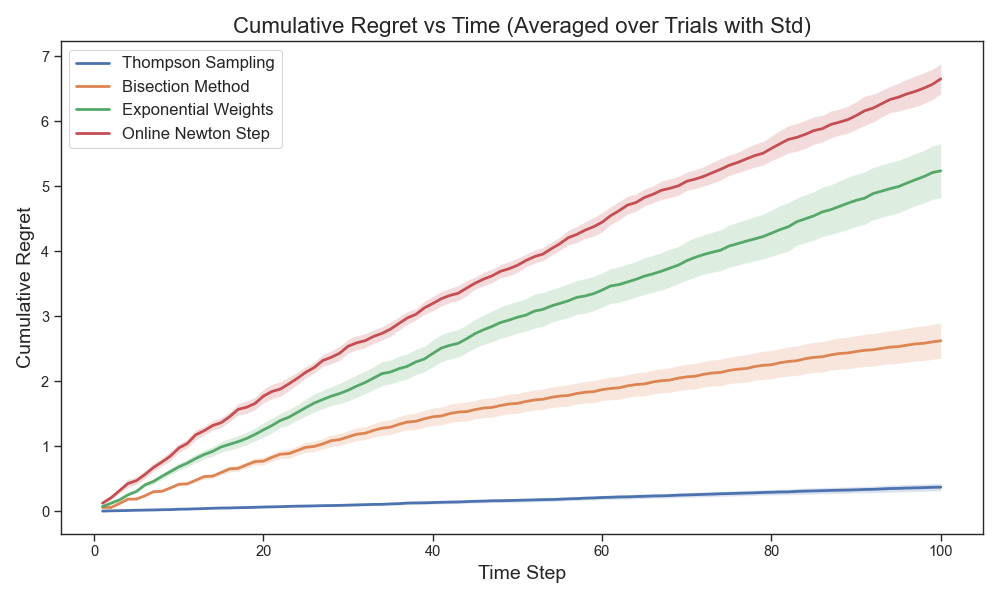
\includegraphics[width=0.8\textwidth]{figures/bayesian_regret.png}
    \caption{Bayesian regret for 1-dimensional bandit convex optimization.
        The plot shows the cumulative regret over $n = 100$ rounds, averaged over 10 independent runs.
        The loss functions are sampled from a multivariate Gaussian prior with $d = 100$ basis functions,
        and observations are corrupted with Gaussian noise $\mathcal{N}(0, 0.1^2)$.}
    \label{fig:bayesian-regret}
\end{figure}
First we study Bayesian regret.
We first sample $\theta_\star$ from a multivariate Gaussian distribution
that is known to the learner.
We set the observation noise $\mathcal{N}(0, \sigma^2)$
with $\sigma = 0.1$.
The number of basis functions is set to $d = 100$.
We run the experiment for $n = 100$ rounds,
and report the average performance over $10$ runs in Figure~\ref{fig:bayesian-regret}.
The performance is compared to the Bisection Method \citep{agarwal2010optimal},
the Exponential Weights with kernel estimation \citep{BEL16}, and
Online Newton Step \citep{LFMV24-improved}.
The superiority of \ts can be explained by the fact that
it is able to use the knowledge of prior, and also the fact that
most of the other algorithms are designed for the adversarial setting primarily.

\section{Regret Against Specific Losses}
\label{sec:ts-empirical-results-regret}
One might wonder how well \ts will perform if the
loss function is not sampled from the prior $\xi$,
and is instead fixed to a specific function $f_\star$.
We study three loss functions:
\begin{enumerate}
    \item Absolute loss: $f_\star(x) = m\abs{x - c}$, for some $c \in [-1, 1]$ and $m > 0$.
    \item Quadratic loss: $f_\star(x) = m(x - c)^2$, for some $c \in [-1, 1]$ and $m > 0$.
    \item Linear loss: $f_\star(x) = mx + b$, such that $\inf_{x \in [-1, 1]} f_\star(x) \geq 0$.
\end{enumerate}
We show the behavior of \ts alongside other algorithms in Fig~\ref{fig:specific-losses}.
The dashed lines are functions $f_t$ that are sampled from
$\xi_t$ for $t \in [100]$, with newer samples been drawn
with higher color density.
The circles are the actions taken by different algorithms
(the color specify the algorithm) with bigger circles
showing more recent actions.
\begin{figure}[h!]
    \centering
    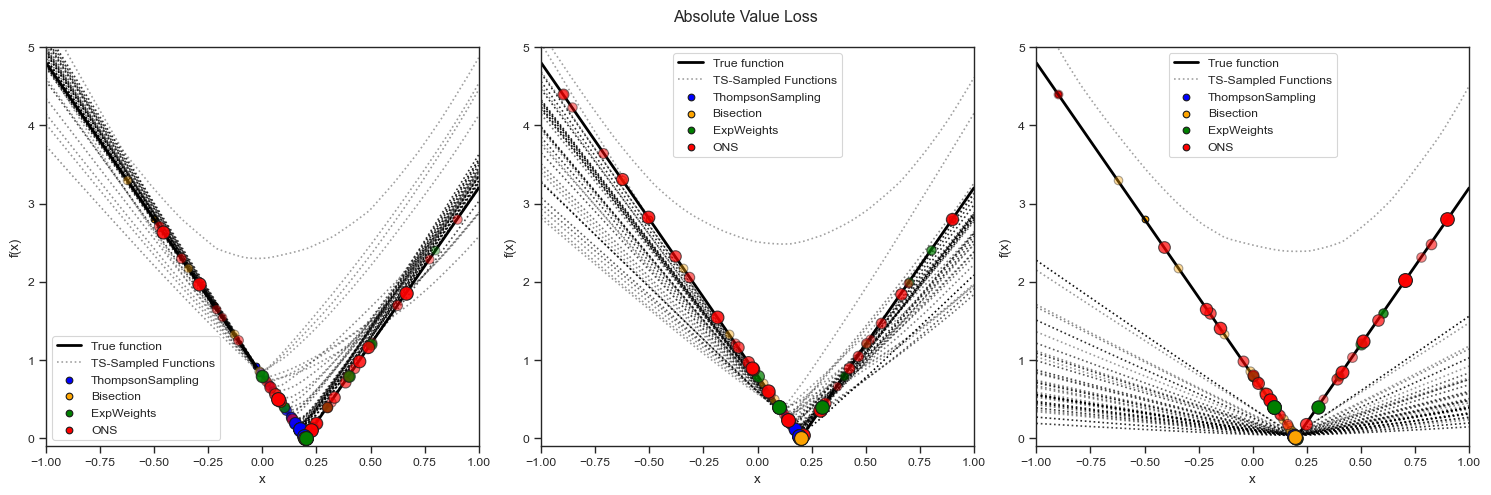
\includegraphics[width=\textwidth]{figures/absolute.png}

    \vspace{0.5em}
    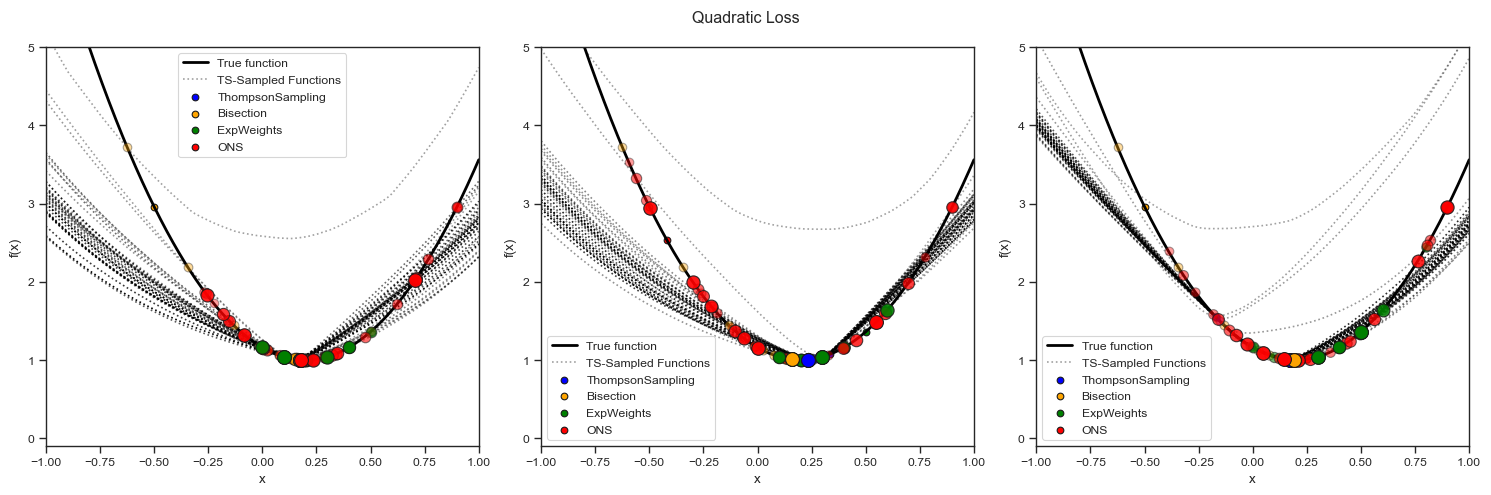
\includegraphics[width=\textwidth]{figures/quadratic.png}

    \vspace{0.5em}
    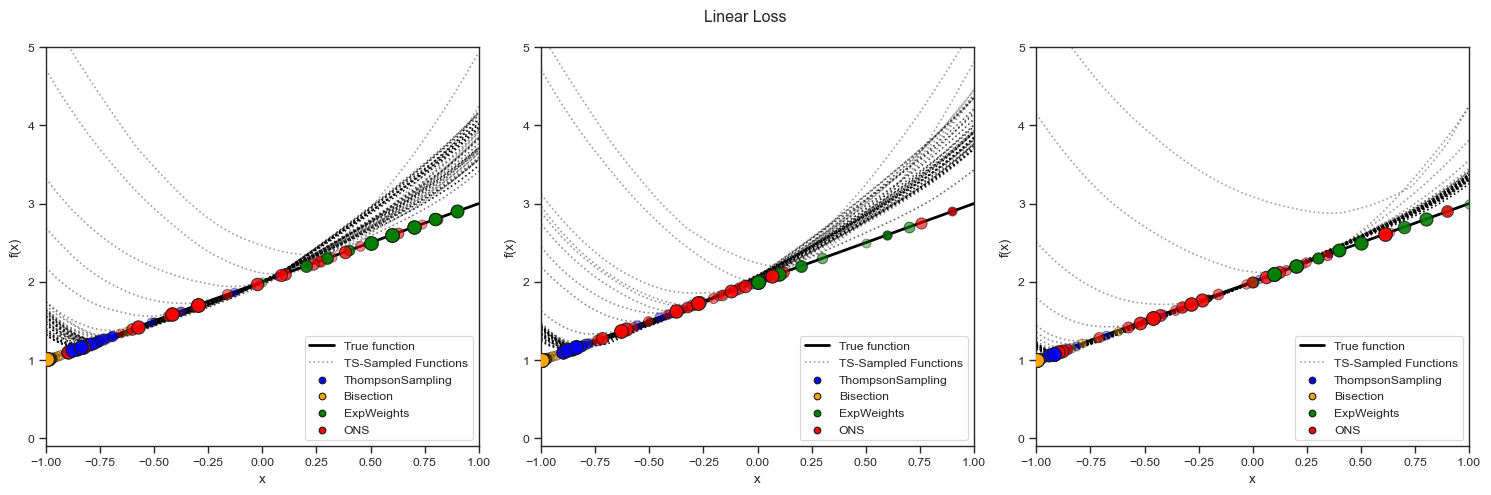
\includegraphics[width=\textwidth]{figures/linear.png}

    \caption{
        Performance of \bco algorithms against specific loss functions.
        Top: Absolute loss $f_\star(x) = m|x - c|$.
        Middle: Quadratic loss $f_\star(x) = m(x - c)^2$.
        Bottom: Linear loss $f_\star(x) = mx + b$.
        Solid line shows $f_\star$, dashed lines show \ts sampled functions,
        and circles show actions taken by different algorithms.
    }
    \label{fig:specific-losses}
\end{figure}

The regret of different algorithms against these losses is pictured
in Fig~\ref{fig:specific-losses-reg}.
It can be seen that \ts remains highly competitive even when
the losses are chosen in an arbitrary way.
\begin{figure}[h!]
    \centering
    \begin{subfigure}{10cm}
        \centering
        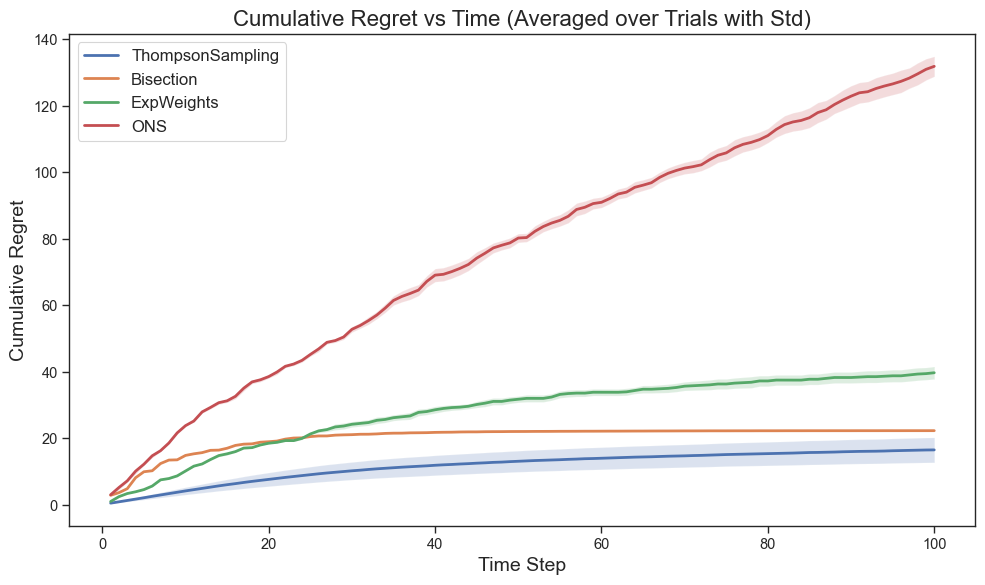
\includegraphics[width=\textwidth]{figures/absolute_reg.png}
        \caption{Average regret against absolute loss: $f_\star(x) = m|x - c|$}
        \label{fig:absolute-loss-regret}
    \end{subfigure}

    \vspace{0.5em}
    \begin{subfigure}{10cm}
        \centering
        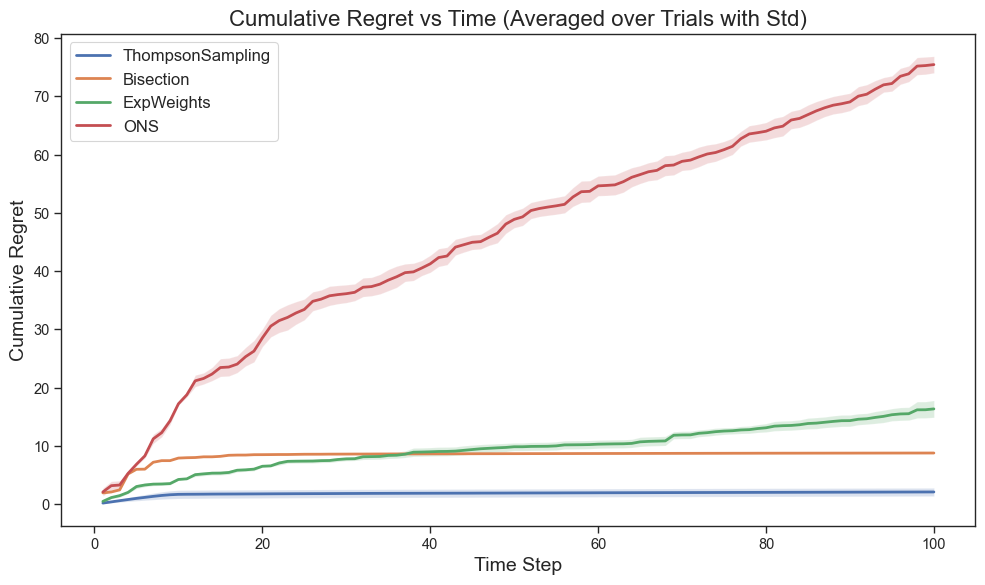
\includegraphics[width=\textwidth]{figures/quad_reg.png}
        \caption{Average regret against quadratic loss: $f_\star(x) = m(x - c)^2$}
        \label{fig:quadratic-loss-regret}
    \end{subfigure}

    \vspace{0.5em}
    \begin{subfigure}{10cm}
        \centering
        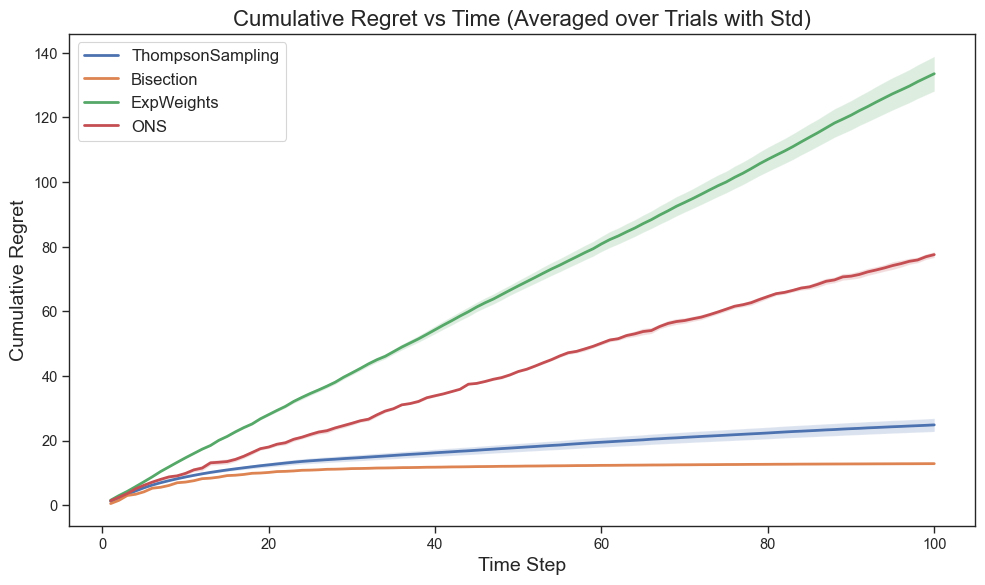
\includegraphics[width=\textwidth]{figures/linear_reg.png}
        \caption{Average regret against linear loss: $f_\star(x) = mx + b$}
        \label{fig:linear-loss-regret}
    \end{subfigure}
    \caption{Average regret of \ts and other algorithms against specific loss functions.}
    \label{fig:specific-losses-reg}
\end{figure}


\chapter{Thompson Sampling for Adversarial Problems}
\label{ch:ts-adv}
In the Bayesian adversarial setting the prior is a probability measure on $\sF^n$ and a whole sequence of loss functions is sampled in secret
by the environment.
The natural generalisations of \ts{} in this setting are the following:
\begin{enumerate}
    \item Sample $(f_s)_{s=1}^n$ from the posterior and play $X_t = \argmin_{x \in \cK} f_t(x)$. \label{item:ts-adv:bad}
    \item Sample $(f_s)_{s=1}^n$ from the posterior and play $X_t = \argmin_{x \in \cK} \sum_{s=1}^t f_s(x)$. \label{item:ts-adv:ok}
\end{enumerate}
The version in \ref{item:ts-adv:bad} suffers linear regret as the following example shows.
Let $d = 1$ and $\cK = [-1,1]$ and $f(x) = \epsilon + \max(\epsilon x, (1 - \epsilon) x)$ and $g(x) = f(-x)$.
Note that $f \in \sF_{\pb\pl}$ and is piecewise linear and minimised at $-1$ with $f(-1) = 0$ and $f(0) = \epsilon$ and $f(1) = 1$.
The function $g$ is the mirror image of $f$.
Now let $\nu$ be the uniform distribution on $\{f, g\}$ and $\xi = \nu^n$ be the product measure.
\ts{} as defined in \ref{item:ts-adv:bad} plays uniformly on $\{1, -1\}$ and an elementary calculation shows that the regret
is $\Omega(n)$.

\begin{figure}[h!]
    \centering
    \begin{tikzpicture}
        \begin{axis}[
                xlabel={$x$},
                % ylabel={$f(x)$},
                domain=-1:1,
                samples=200,
                width=7cm,
                height=4cm,
                % legend pos=north west,
                % legend style={at={(0.5,-0.2)},anchor=north},
                axis x line=middle,
                axis y line=middle,
                xtick={-1,0,0.25,1},
                ytick={0,0.5,1,1.5,2},
                xticklabels={$-1$,$0$,$0.25$,$1$},
                yticklabels={$0$,$0.5$,$1$,$1.5$,$2$},
                xmin=-1,
                xmax=1,
                ymin=0,
                ymax=1.1,
            ]
            % Plot the original function f(x)=0.2+0.8*x^2 in blue.
            \addplot [blue,  thick] {0.2+0.8*x^2 + 0.01};
            % \addlegendentry{$f(x)=\epsilon+(1-\epsilon)x^2,\; \epsilon=0.2$};

            % For theta=0.25, we have sqrt(epsilon/(1-epsilon))=sqrt(0.2/0.8)=0.5.
            % f_{0.25}(x) is defined as follows:
            % For x in [-0.25,0.25]:
            %   f_{0.25}(x)= (1-\epsilon)\Bigl(\theta^2 + 2\,(x-\theta)(\theta-\sqrt{\epsilon/(1-\epsilon)})\Bigr)
            %             = 0.8*(0.0625 - 0.5*(x-0.25))
            \addplot [red,  thick, domain=-0.25:0.25] {0.8*(0.0625 - 0.5*(x-0.25)) -0.01};

            % For x in [0.25,0.75]:
            %   f_{0.25}(x)= (1-\epsilon)\Bigl(\theta^2 + 2\,(x-\theta)(\theta+\sqrt{\epsilon/(1-\epsilon)})\Bigr)
            %             = 0.8*(0.0625 + 1.5*(x-0.25))
            \addplot [red,  thick, domain=0.25:0.75] {0.8*(0.0625 + 1.5*(x-0.25)) -0.01};

            % For x outside [-0.25,0.75], f_{0.25}(x) equals f(x).
            \addplot [red,  thick, domain=-1:-0.25] {0.2+0.8*x^2 - 0.01};
            \addplot [red,  thick, domain=0.75:1] {0.2+0.8*x^2 - 0.01};
            % \addlegendentry{$f_{0.25}(x)$, $\theta=0.25,\ \epsilon=0.2$};

            % Optional: Add dashed vertical lines to mark the breakpoints.
            \draw[dashed] (axis cs:-0.25,0) -- (axis cs:-0.25,{0.2+0.8*(-0.25)^2});
            \draw[dashed] (axis cs:0.75,0) -- (axis cs:0.75,{0.2+0.8*(0.75)^2});

            % add a vertical line at theta=0.25 to mark the value of theta.
            \draw[dashed] (axis cs:0.25,0) -- (axis cs:0.25,{0.8*(0.25)^2});

            \node [blue] at (axis cs:0.7,0.9) {$f(x)$};
            \node [red] at (axis cs:-0.7,0.3) {$f_{0.25}(x)$};
        \end{axis}
    \end{tikzpicture}
    \caption{
        The function $f(x) = 0.2 + 0.8 x^2$ and the function $f_{0.25}$ with $\epsilon = 0.2$.
        The function $f_{0.25}$ is the largest convex function that is smaller than $f$ and has $f_{0.25}(0.25) = f(0.25) - 0.2$.
    }
    \label{fig:adversarial-lower-bound}
\end{figure}
We do not know if the version of \ts{} defined in \ref{item:ts-adv:ok} has $\tilde O(\sqrt{n})$ Bayesian regret.
% But \cite{BDKP15} note that at least naively the information-theoretic machinery is not suitable for analysing this algorithm.
However, the following example shows that in general the adversarial version of the information ratio is not bounded.
Because the loss function changes from round to round, the action $X_t$ may not minimise $f_t$. This must be reflected in the definition of the information
ratio. Let $\xi$ be a probability measure on $\sF \times \cK$ and $\pi$ be a probability measure on $\cK$ and let
\begin{align*}
    \Delta(\pi, \xi) = \E[f(X) - f(X_\star)]  \qquad \text{ and } \qquad
    \I(\pi, \xi) = \E[(f(X) - \E[f(X)|X])^2]\,,
\end{align*}
where $(f, X_\star, X)$ has law $\xi \otimes \pi$.
Thompson sampling as in \cref{item:ts-adv:ok} is the policy $\pi$ with the same law as $X_\star$. The claim is that in general it does not hold
that
\begin{align*}
    \Delta(\pi, \xi) \leq \alpha + \sqrt{\beta \I(\pi, \xi)}\,,
\end{align*}
unless $\alpha$ is unreasonably large.
Let $d = 1, \epsilon \in (0, 2^{-7}), \cK = [-1,1]$, and $f(x) = \epsilon + (1 - \epsilon) x^2$.
Given $\theta \in [-1,1]$ let $f_\theta(x)$ be defined as
\begin{align*}
    f_\theta(x) = \begin{cases}
                      (1-\epsilon) (\theta^2 + 2 (x - \theta)(\theta + \sqrt{\frac{\epsilon}{1-\epsilon}}))
                           & \theta \leq x \leq \theta + \sqrt{\frac{\epsilon}{1-\epsilon}} \\
                      (1-\epsilon) (\theta^2 + 2 (x - \theta)(\theta - \sqrt{\frac{\epsilon}{1-\epsilon}}))
                           & \theta - \sqrt{\frac{\epsilon}{1-\epsilon}} \leq x < \theta    \\
                      f(x) & \text{otherwise},
                  \end{cases}
\end{align*}
which is convex and smaller than $f$ for all $x \in \cK$.
Essentially, $f_\theta$ should be thought of as the largest convex function
that is smaller than $f$ and has $f_\theta(\theta) = f(\theta) - \epsilon$
(see \cref{fig:adversarial-lower-bound}).
Moreover, an elementary calculation shows that $\max_{x \in \cK} |f(x) - f_\theta(x)| = \epsilon$ for all $\theta \in [-1,1]$.
Let $\xi$ be the law of $(f_\theta, \theta)$ when $\theta$ is sampled uniformly from $[-1,1]$ and $\pi$ be uniform on $[-1,1]$ which is the \ts{}
policy as defined in \ref{item:ts-adv:ok}.
Then, by letting $\theta'$ be an i.i.d. copy of $\theta$ we have
\begin{align*}
    \Delta(\pi, \xi)
     & =
    \E\brak{
        f_{\theta}(\theta') - f_\theta(\theta)
    }
    =
    \E\brak{
        f_{\theta}(\theta') - f(\theta)
    } + \epsilon
    =
    \E\brak{
        f_{\theta'}(\theta) - f(\theta)
    } + \epsilon
\end{align*}
where the second equality follows from the definition of $f_\theta$ and the third equality follows from $f_\theta(\theta) = f(\theta) - \epsilon$.
Next, we have
\begin{align*}
    \E\brak{
        f_{\theta'}(\theta) - f(\theta)
    }
     & =
    \E\brak{
        \sind_{
            \left\{
            |\theta - \theta'| \leq \sqrt{\frac{\epsilon}{1-\epsilon}}
            \right\}
        }
        \paren{
            f_{\theta'}(\theta) - f(\theta)
        }
        +
        \sind_{
            \left\{
            |\theta - \theta'| \geq \sqrt{\frac{\epsilon}{1-\epsilon}}
            \right\}
        }
        \paren{
            f_{\theta'}(\theta) - f(\theta)
        }
    }    \\
     &
    \explan{(a)}
    =
    \E\brak{
        \sind_{
            \left\{
            |\theta - \theta'| \leq \sqrt{\frac{\epsilon}{1-\epsilon}}
            \right\}
        }
        \paren{
            f_{\theta'}(\theta) - f(\theta)
        }
    }
    \\
     &
    \explan{(b)}
    \geq
    -
    \mathbb{P}\paren{
        |\theta - \theta'| \leq \sqrt{\frac{\epsilon}{1-\epsilon}}
    }
    \epsilon
    \\
     &
    \explan{(c)}
    \geq
    -
    2 \sqrt{\frac{\epsilon}{1-\epsilon}}
    \epsilon\,,
\end{align*}
where \texttt{(a)} follows from the fact that $f_{\theta'}(\theta) = f(\theta)$
if $|\theta - \theta'| \geq \sqrt{\frac{\epsilon}{1-\epsilon}}$;
\texttt{(b)} follows from the fact that $f_{\theta'} \leq f(\theta)$
and the fact that $\max_{x \in \cK} |f(x) - f_\theta(x)| = \epsilon$;
and \texttt{(c)} follows from the fact that $\theta$ and $\theta'$ are i.i.d. on $[-1,1]$.
Therefore,
\begin{align*}
    \Delta(\pi, \xi)
    \geq
    \epsilon \paren{1 - 2 \sqrt{\frac{\epsilon}{1-\epsilon}}}\,.
\end{align*}
Next, we turn our attention to $\I(\pi, \xi)$, which can be upper bounded as
\begin{align*}
    \I(\pi, \xi)
     & =
    \E\brak{
        \paren{
            f_{\theta'}(\theta) - \E\brak{f_{\theta'}(\theta)|\theta}
        }^2
    }
    \\
     &
    \explan{(a)}
    \leq
    \E\brak{
        \paren{
            f_{\theta'}(\theta) - f(\theta)
        }^2
    }
    \\
     &
    \explan{(b)}
    \leq
    \mathbb{P}\paren{
        |\theta - \theta'| \leq \sqrt{\frac{\epsilon}{1-\epsilon}}
    }
    \epsilon^2
    \\
     &
    \explan{(c)}
    \leq
    2 \epsilon^2\sqrt{\frac{\epsilon}{1-\epsilon}}\,,
\end{align*}
where \texttt{(a)} follows from the fact that the mean minimizes the squared deviation;
\texttt{(b)} follows from the fact that $f_{\theta'}(\theta) = f(\theta)$
if $|\theta - \theta'| \geq \sqrt{\frac{\epsilon}{1-\epsilon}}$;
and \texttt{(c)} follows from the fact that $\theta$ and $\theta'$ are i.i.d. on $[-1,1]$.
Therefore, by putting the two inequalities together we have
\begin{align*}
    \frac{
        \Delta(\pi, \xi)
    }{
        \sqrt{\I(\pi, \xi)}
    }
    \geq
    \frac{
        \epsilon \paren{1 - 2 \sqrt{\frac{\epsilon}{1-\epsilon}}}
    }{
        \sqrt{2 \epsilon^2\sqrt{\frac{\epsilon}{1-\epsilon}}}
    }
    =
    \frac{
        1 - \sqrt{\frac{4\epsilon}{1-\epsilon}}
    }{
        \sqrt[4]{\frac{4\epsilon}{1-\epsilon}}
    }
    =
    \sqrt[4]{\frac{1-\epsilon}{4\epsilon}}
    -
    \sqrt[4]{\frac{4\epsilon}{1-\epsilon}}\,,
\end{align*}
which can be further lower bounded by
\begin{align*}
    \frac{
        \Delta(\pi, \xi)
    }{
        \sqrt{\I(\pi, \xi)}
    }
    \geq
    \sqrt[4]{\frac{1-\epsilon}{4\epsilon}}
    -
    \sqrt[4]{\frac{4\epsilon}{1-\epsilon}}
    \geq
    \sqrt[4]{\frac{1}{4\epsilon} - \frac{1}{4}}
    -
    \sqrt[4]{8\epsilon}
    \geq
    \sqrt[4]{\frac{1}{8\epsilon}}
    -
    \sqrt[4]{8\epsilon}
    \geq
    \frac{1}{4}\epsilon^{-\frac14}\,,
\end{align*}
where the all inequalities follow from $\epsilon \in (0,2^{-7})$.
Therefore, the information ratio is unbounded as $\epsilon \to 0$.

\chapter{Discussion}
In this thesis, we explored the performance of Thompson sampling (\ts) for Bayesian bandit convex optimization (\bco), revealing a nuanced picture of its capabilities.
We established its near-optimal performance in one-dimensional
settings and for the class of monotone ridge functions,
demonstrating its efficacy in structured scenarios.
In stark contrast, we also showed that \ts can fail dramatically
in general high-dimensional problems and that standard analytical tools
face fundamental limitations.
This chapter synthesizes these findings, discusses their broader implications
for algorithm design in online optimization,
and explores the structural properties that determine the success or
failure of \ts.


\section{Adversarial setup} In the Bayesian adverarial setting a sequence of loss functions $f_1,\ldots,f_n$ are sampled from a joint distribution on $\sF^n$.
The learner plays $X_t$ and observes $Y_t = f_t(X_t)$ and the Bayesian regret is
$\BReg(\sA, \xi) = \E[\sup_{x \in \cK} \sum_{t=1}^n (f_t(X_t) - f_t(x))]$.
One can envisage two possible definitions of Thompson sampling in this setting. One samples $g_t$ from the marginal of the posterior and plays $X_t = x_{g_t}$.
The second samples $g_1,\ldots,g_n$ from the posterior and plays $X_t$ as the minimiser of $\sum_{t=1}^n g_t$.
The former has linear regret, while \cite{BDKP15} notes
that the latter has an unbounded information ratio. The situation was discussed in more details in \cref{ch:ts-adv}.
\section{Tightness of bounds} At present we are uncertain whether or not the monotonicity assumption is needed in the ridge setting. Our best guess is that it is not.
One may also wonder if the bound on the information ratio in \cref{thm:ridge-ir} can be improved. We are cautiously believe
that when the loss has the form $f(x) = \ell(\ip{x, \theta})$ for \textit{known} convex link function $\ell : \R \to \R$, then the information ratio is at most $d$.
This would mean that convex generalised linear bandits are no harder than linear bandits.

\section{\ts{} vs \IDS} \cref{thm:ts-lower} shows that \ts{} can have more-or-less linear regret in high-dimensional problems. On the other hand,
\cite{BE18} and \cite{Lat20-cvx} show that \IDS{} has a well-controlled information ratio, but is much harder to compute.
An obvious question is whether some simple adaptation of Thompson sampling has a well-controlled information ratio.
\section{Applications} Many problems are reasonably modelled as $1$-dimensional convex bandits, with the classical example being dynamic pricing
where $\cK$ is a set of prices and convexity is a reasonable assumption based on the response of demand to price.
The monotone ridge function class is a natural model for resource allocation problems where a single resource (e.g., money) is allocated to $d$ locations.
The success of some global task increases as more resources are allocated, but with diminishing returns. Problems like this can reasonably be modelled
by convex monotone ridge functions with $\cK = \{x \geq \zeros : \norm{x}_1 \leq 1\}$.
\section{Lipschitz assumption} Our bounds depend logarithmically on the Lipschitz constant associated with the class of loss functions.
There is a standard trick to relax this assumption based on the observation that bounded convex functions must be Lipschitz on a suitably defined
interior of the constraint set $\cK$.
Concretely, suppose that $\cK$ is a convex body and $f : \cK \to [0,1]$ is convex and $\ball_r \subset \cK$ and $\cK_\epsilon = (1 - \epsilon) \cK$.
Then $\min_{x \in K_\epsilon} f(x) \leq \inf_{x \in \cK} f(x) + \epsilon$ and $f$ is $1/(r\epsilon)$-Lipschitz on $K_\epsilon$ \citep[Chapter 3]{lat24book}.
Hence, you can run \ts{} on $K_\epsilon$ with $\epsilon = 1/n$ and the Lipschitz constant is at most $n/r$.
Moreover, if $\cK$ is in (approximate) isotropic or John's position, then $\ball_1 \subset \cK \subset \ball_{2d}$ by \cite{kannan1995isoperimetric}
and John's theorem, respectively.

\section{Frequentist regret}
An ambitious goal would be to prove a bound on the frequentist regret of \ts{} for some well-chosen prior.
This is already quite a difficult problem in multi-armed \citep{KKM12,AG12b} and linear bandits \citep{AG13} and is out of reach of the techniques developed here.
On the other hand, the Bayesian algorithm has the advantage of being able to specify a prior that makes use of background knowledge and the theoretical guarantees
for \ts{} provide a degree of comfort.

\section{Choice of prior} The choice of the prior depends on the application. A variety of authors constructed priors supported on non-parametric
classes of $1$-dimensional convex functions
using a variety of methods \citep{ramgopal1993nonparametric,chang2007shape,shively2011nonparametric}.
In many cases you may know the loss belongs to a simple parametric class, in which case the prior and posterior computations may simplify dramatically.

% \part{Anytime Estimation to Decision Algorithm}
% \chapter{Decision Making With Structured Observations}
% Regret minimization is a widely studied objective in bandits and reinforcement learning theory \citep{lattimore2020bandit} that has inspired practical algorithms,
% for example, in noisy zero-order optimization\citep[e.g.,][]{SKK10} and deep reinforcement learning \citep[e.g.,][]{osband2016deep}.
% Cumulative regret measures the online performance of the algorithm by the total loss suffered due to choosing suboptimal decisions.
% Regret is unavoidable to a certain extent as the learner collects information to reduce uncertainty about the environment.
% In other words, a learner will inevitably face
% the exploration-exploitation trade-off where it must balance collecting rewards and collecting information. Finding the right balance is the central challenge of sequential decision-making under uncertainty.\looseness=-1
% In this part of the thesis, we study the problem of regret minimization in sequential decision-making with structured observations, as defined in the following section.

% \section{Problem Setup}
% More formally, denote by $\Pi$ a decision space and $\cO$ an observation space. Let $\cH$ be a class of models, where $f = (r_f, M_f) \in \cH$ associated with a reward function $r_f : \Pi \rightarrow \R$ and observation map $M_f : \Pi \rightarrow \cP(\cO)$,
% where $\cP(\cO)$ is the set of all probability distributions over $\cO$.%
% \footnote{To simplify the presentation, we ignore tedious measure-theoretic details in this part. The reader could either fill out the missing details, or just assume that all sets, unless otherwise stated, are discrete.}
% %\todoc{So I said we ignore measure theory. Sometimes this is easy. However, one may need additional structure of one talks about policies obtained with argmin (the question of ``measurable selection''). When things are discrete, all is fine. And also in Polish spaces.. Do not ask me about other settings.}
% The learner's objective is to collect as much reward as possible in $n$ steps when facing a model $f^* \in \cH$. The learner's prior information is $\cH$ and the associated reward and observation maps, but does not know the true instance $f^* \in \cH$.
% The learner constructs a stochastic sequence $\pi_1, \dots, \pi_n$ of decisions taking values in $\Pi$ and adapted to the history of observations $y_t \sim M_{f^*}(\pi_t)$.
% %: $\pi_t$ is chosen stochastically as a function of $(\pi_1,y_1,\dots,\pi_{t-1},y_{t-1})$. 
% The policy of the learner is the sequence of probability kernels $\mu_{1:n} = (\mu_t)_{t=1}^n$ that are used to take decisions.
% %Note that the policy of a learner is independent of the true unknown model $f^*$.
% The expected regret of a policy $\mu_{1:n}$ and model $f^*$ after $n \in [N]$ steps is
% \begin{align*}
%     R_n(\mu_{1:n}, f^*) = \max_{\pi \in \Pi} \E\left[\sum_{t=1}^n  r_{f^*}(\pi) - r_{f^*}(\pi_t)\right]
% \end{align*}
% The literature studies regret minimization for various objectives, including worst-case and instance-dependent frequentist regret \citep{lattimore2020bandit}, Bayesian regret \citep{RV16} and robust variants \citep{garcelon2020adversarial,kirschner2020distributionally}.
% For the frequentist analysis, all prior knowledge is encoded in the model class $\cH$.
% The worst-case regret of policy $\mu_{1:n}$ on $\cH$ is $\sup_{f \in \cH} R_n(\mu_{1:n}, f)$, and therefore the optimal minimax regret $\inf_\mu \sup_{f \in \cH} R_n(\mu_{1:n}, f)$ only depends on $\cH$ and the horizon $n$.
% The Bayesian, in addition, assumes access to a prior $\nu \in \cP(\cH)$, which leads to the Bayesian regret $\E_{f \sim \nu}[R_n(\mu_{1:n}, f)]$. Interestingly, the worst-case frequentist regret and Bayesian regret are dual in the following sense
% \citep{LS19pminfo}:\footnote{The result by \citep{LS19pminfo} was only shown for finite action, reward and observation spaces, but can likely be extended to the infinite case under suitable continuity assumptions.}
% % \todoc{also, before our paper there were others noting this in special cases (with incorrect proofs). not sure whether we want to refer to them..}
% \begin{align}
%     \inf_{\mu_{1:n}} \sup_{f \in \cH} R_n(\mu_{1:n}, f) = \sup_{\nu \in \cP(\cH)} \inf_{\mu_{1:n}} \E_{f \sim \nu}[R_n(\mu_{1:n}, f)] \label{eq:freq-bayes-regret}
% \end{align}
% Unfortunately, directly solving for the minimax policy (or the worst-case prior) is intractable, except in superficially simple problems.
% This is because the optimization is over the exponentially large space of adaptive policies.
% However, the relationship in \cref{eq:freq-bayes-regret} has been directly exploited in prior works, for example, to derive non-constructive upper bounds on the worst-case regret via a Bayesian analysis \citep{BDKP15}.
% Moreover, it can be seen as inspiration underlying ``optimization-based'' algorithms for regret minimization: The crucial step is to carefully relax the saddle point problem in a way that preserves the statistical complexity, but can be analyzed and computed more easily.
% This idea manifests in several closely related algorithms,
% including information-directed sampling \citep{RV14,kirschner2018information},
% ExpByOpt \citep{lattimore2020exploration,lattimore2021mirror}, and most recently,
% the \mbox{Estimation-To-Decisions (E2D)}
% framework \citep{foster2021statistical,foster2023tight}.
% These algorithms have in common that they optimize the information trade-off directly, which in structured settings leads
% to large improvements compared to standard optimistic exploration approaches and Thompson sampling.
% Yet, the precise relation among the different approaches are not yet fully understood.
% On the other hand, algorithms that directly optimize the information trade-off can be computationally more demanding and, consequently, are often not the first choice of practitioners. This is partly due to the literature primarily focusing on statistical aspects, leaving computational and practical considerations underexplored.

% \subsection{Related Work}

% There is a broad literature on regret minimization in bandits \citep{lattimore2020bandit} and reinforcement learning
% \citep{jin2018q, azar2017minimax, zhou2021nearly, du2021bilinear, zanette2020learning}.
% Arguably the most popular approaches are based on optimism, leading to the widely analysed upper confidence bound (UCB) algorithms \citep{lattimore2020bandit}, and Thompson sampling (TS) \citep{thompson1933likelihood,RV16}.

% A long line of work approaches regret minimization as a saddle point problem. \cite{degenne2020games} showed that in the structured bandit setting, an algorithm based on solving a saddle point equation achieves asymptotically optimal regret bounds, while explicitly controlling the finite-order terms. \cite{lattimore2020exploration} propose an algorithm based on exponential weights in the partial monitoring setting \citep{rustichini1999minimizing} that finds a distribution for exploration by solving a saddle-point problem.  The saddle-point problem balances the trade-off between the exponential weights distribution and an information or stability term.
% The same approach was further refined by \cite{lattimore2021mirror}. In stochastic linear bandits, \cite{kirschner2021asymptotically} demonstrated that information-directed sampling can be understood as a primal-dual method solving the asymptotic lower bound, which leads to an algorithm that is both worst-case and asymptotically optimal. The saddle-point approach has been further explored in the PAC setting \citep[e.g.,][]{degenne2020games,degenne2020gamification}.

% The work in this part or the thesis is closely related to recent work by \cite{foster2021statistical, foster2023tight}.
% They consider \textit{decision making with structured observations} (DMSO), which generalizes the bandit and RL setting.
% They introduce a complexity measure, the \textit{offset decision-estimation coefficient} (offset DEC), defined as a min-max game between a learner and an environment, and provide lower bounds in terms of the offset DEC.
% Further, they provide an algorithm, \textit{Estimation-to-Decisions} (E2D) with corresponding worst-case upper bounds in terms of the offset DEC.
% Notably, the lower and upper bound nearly match and recover many known results in bandits and RL.
% The offset DEC is
% More recently, \cite{foster2023tight} refined the previous bounds by introducing the \emph{constrained} DEC
% and a corresponding algorithm E2D$^+$.
% Although achieving better bounds, this algorithm and the analysis is significantly more involved than for the E2D algorithm.

% There are various other results related to the DEC and the E2D algorithm.
% \cite{foster2022note} show that the E2D achieves improved bounds in model-free RL when combined with optimistic estimation (as introduced by \cite{zhang2022feel}).
% \cite{chen2022unified} introduced two new complexity measures based on the DEC that are necessary and sufficient for reward-free learning and PAC learning.
% They also introduced new algorithms based on the E2D algorithm for the above two settings and various other improvements.
% \cite{foster2022complexity} have shown that the DEC is necessary and sufficient to obtain low regret for \textit{adversarial} decision-making.
% An asymptotically instance-optimal algorithm for DMSO has been proposed by \cite{dong2022asymptotic}, extending a similar approach for the linear bandit setting \citep{lattimore2017end}. %However, this approach is not worst-case optimal.
% % \cite{zhong2022posterior} introduce a different complexity measure, the \textit{Generalized Eluder Coefficient} (GEC), which was used to provide regret bounds for more general problems such as partially observable MDPs.
% %However, they were unable to provide any regret lower bounds, justifying the necessity of the GEC.
% %Important, is that none of the above mentioned works address the same issues we are interested in, namely, finding a simple, and practical algorithm for the stochastic setting that can adapt to the problem instance.

% The decision-estimation coefficient is also related to the information ratio \citep{RV14} and the decoupling coefficient \citep{zhang2022feel}. The information ratio has been studied under both the Bayesian \citep{RV14} and the frequentist regret \citep{kirschner2018information,kirschner2020linearpm, kirschner2021asymptotically, kirschner2023linear} in various settings including bandits, reinforcement learning, and partial monitoring. The decoupling coefficient was studied for the Thompson sampling algorithm in contextual bandits \citep{zhang2022feel}, and RL \citep{dann2021provably,agarwal2022model}.

% \section{The Problem Setup}
% Recall that $\Pi$ is a compact decision space and $\cO$ is an observation space. The model class $\cH$ is a set of tuples $f = (r_f, M_f)$ containing a reward function $r_f : \Pi \rightarrow \R$ and an observation distribution $M_f : \Pi \rightarrow \sP(\cO)$.
% Further bounded- and finiteness assumptions will be introduced in the context of the relevant statements.
% We make the assumption that both $\cH$ and $\Pi$ are finite, however, our results extend to continuous action and hypothesis spaces under appropriate technical conditions using standard arguments.
% In particular, the sample complexity bounds we provide scale with $\log(|\cH|)$ in many cases, facilitating covering arguments for the continuous setting.
% Computationally, we will assume that $\cH$ can be computationally enumerated (or rely on subsampling).
% While this is a strong assumption, it is less clear under what conditions one can achieve better results; and even the case where $\cH$ is finite, computational aspects of E2D have not been explored in the literature.
% We define the gap function
% \begin{align}
%     \Delta(\pi, g) = r_g(\pi_g^*) - r_g(\pi) \, , \nonumber
% \end{align}
% where $\pi^*_g = \argmax_{\pi \in \Pi} r_g(\pi)$ is an optimal decision for model $g$, chosen arbitrarily if not unique.
% A randomized policy is a sequence of kernels $\mu_{1:n} = (\mu_t)_{t=1}^n$ from histories $h_{t-1} = (\pi_1,y_1,\dots,\pi_{t-1},y_{t-1}) \in (\Pi \times \cO)^{t-1}$ to sampling distributions $\sP(\Pi)$. The filtration generated by the history $h_t$ is $\cF_t$.
% The learner's decisions $\pi_1, \dots, \pi_n$ are sampled from the policy $\pi_t \sim \mu_t$ and observations $y_t \sim M_{f^*}(\pi_t)$ are generated by an unknown true model $f^* \in \cH$. The expected regret under model $f^*$ is formally defined as follows:
% \begin{align}
%     R_n(\mu_{1:n}, f^*) = \EE[\sum_{t=1}^n \EE_{\pi_t \sim \mu_t(h_t)}[\Delta(\pi_t, f^*)]] \nonumber
% \end{align}
% For now, we do not make any assumption about the reward being observed. This provides additional flexibility to model a wide range of scenarios, including for example, duelling and ranking feedback~\citep{YJ09,radlinski08learning,combes15learning,LKLS18,kirschner2021dueling}
% (e.g.~used in reinforcement learning with human feedback, RLHF) or dynamic pricing\citep{denBoer15}.
% The setting is more widely known as partial monitoring \cite{rustichini1999minimizing}.
% The special case where the reward is part of the observation distribution is called  \emph{decision-making with structured observations} \cite[DMSO,][]{foster2021statistical}. Earlier work studies the closely related \emph{structured bandit} setting \citep{combes2017minimal}.

% A variety of examples across bandit models and reinforcement learning are discussed in \citep{combes2017minimal,foster2021statistical,foster2023tight,kirschner2023linear}. For the purpose of this part, we focus on simple cases for which we can provide tractable implementations. Besides the finite setting where $\cM$ can be enumerated, these are the following linearly parametrized feedback models.


% \begin{example}[Linear Bandits, \cite{abe1999associative}]\label{ex:linear-bandits}
%     The model class is identified with a subset of $\bR^d$ and features $\phi_\pi \in \bR^d$ for each $\pi \in \Pi$. The reward function is $r_f(\pi) = \ip{\phi(\pi), f}$ and the observation distribution is $M_f(\pi) = \cN(\ip{\phi_\pi, f}, 1)$.
% \end{example}

% The linear bandit setting can be generalized by separating reward and feedback maps, which leads to the \emph{linear partial monitoring} framework \citep{lin2014combinatorial,kirschner2020linearpm}. Here we restrict our attention to the special case of \emph{linear bandits with side-observations} \citep[c.f.~][]{kirschner2023linear}, which, for example, generalizes the classical semi-bandit setting \cite{mannor2011bandits}

% \begin{example}[Linear Bandits with Side-Observations] \label{ex:semi-bandits}
%     As in the linear bandit setting, we have $\cH\subset \bR^d$, and features $\phi_\pi \in \bR^d$ that define the reward functions $r_f(\pi) = \ip{\phi_\pi, f}$.
%     Observation matrices $M_\pi \in \bR^{m_\pi \times d}$ for each $\pi \in \Pi$ define $m_\pi$-dimensional observation distributions $M_f(\pi) = \cN(M_\pi f, \sigma^2 \eye_{m_\pi})$. In addition, we assume that $\phi_\pi \phi_\pi^\top \preceq M_{\pi}^\top M_\pi$, which is automatically satisfied if $\phi_\pi^\top$ is included in the rows of $M_{\pi}$, i.e. when the reward is part of the observations.
% \end{example}

% \chapter{Regret Minimization via Saddle-Point Optimization}
% The goal of the learner is to choose decisions $\pi \in \Pi$ that achieve a small gap $\Delta(\pi, f^*)$ under the true model $f^* \in \cH$. Since the true model is unknown, the learner has to collect data that provides statistical evidence to reject models $g \neq f^*$ for which the regret $\Delta(\pi, g)$ is large. To quantify the information-regret trade-off, we use a divergence $D(\cdot\|\cdot)$ defined for distributions in $\sP(\cO)$. For a reference model $f$, the information (or divergence) function is defined by:
% \begin{align*}
%     I_{f}(\pi, g) = \KL(M_g(\pi)\| M_{f}(\pi))\,,
% \end{align*}
% where $\KL(\cdot \| \cdot)$ is the KL divergence. Intuitively, $I_f(\pi, g)$ is the rate at which the learner collects statistical information to reject $g \in \cH$ when choosing $\pi \in \Pi$ and data is generated under the reference model $f$. Note that $I_f(\pi, f) = 0$ for all $f\in\cH$ and $\pi \in \Pi$. As we will see shortly, the regret-information trade-off can be written precisely as a combination of the gap function, $\Delta$, and the information function, $I_f$. We remark in passing that other choices such as the Hellinger distance are also possible, and the KL divergence is mostly for concreteness and practical reasons.

% To simplify the notation and emphasize the bilinear nature of the saddle point problem that we study, we will view $\Delta,I_f \in \bR_{+}^{\Pi \times \cH}$ as $|\Pi|\times |\cH|$ matrices (by fixing a canonical ordering on $\Pi$ and $\cH$).
% For vectors $\mu \in \bR^\Pi$ and $\nu \in \bR^\cH$, we will frequently write bilinear forms $\mu \Delta \nu$ and $\mu I_f\nu$. This also means that by convention, $\mu$  will always denote a row vector, while $\nu$ will always denote a column vector.
% The standard basis for $\bR^\Pi$ and $\bR^\cH$ is $(e_\pi)_{\pi \in \Pi}$ and $(e_g)_{g \in \cH}$.

% \subsection{The Decision-Estimation Coefficient}
% To motivate our approach, we recall the \emph{decision-estimation coefficient} (DEC) introduced by \cite{foster2021statistical,foster2023tight}, before introducing the main quantity of interest, the \emph{average-constrained DEC}. First, the \emph{offset decision-estimation coefficient} (without localization) \citep{foster2021statistical} is
% \begin{align}
%     \odec_\lambda(f) = \min_{\mu \in \sP(\Pi)} \max_{g \in \cH} \mu \Delta e_g - \lambda \mu I_{f}e_g \nonumber
% \end{align}
% The tuning parameter $\lambda>0$ controls the weight of the information matrix relative to the gaps:
% Viewing the above as a two-player zero-sum game, we see that increasing $\lambda$ forces the max-player to avoid models that differ significantly from $f$ under the min-player's sampling distribution.
% The advantage of this formulation is that the information term $\mu I_f e_g$ can be telescoped in the analysis, which directly leads to regret bounds in terms of the estimation error (introduced below in \cref{eq:est}).
% The disadvantage of the $\lambda$-parametrization is that the trade-off parameter is chosen by optimizing the final regret upper bound. This is inconvenient because the optimal choice requires knowledge of the horizon and a bound on $\max_{f \in \cH} \rdec^o_{\lambda}(f)$. Moreover, any choice informed by the upper bound may be conservative, leading to sub-optimal performance.

% The \emph{constrained decision-estimation coefficient} \citep{foster2023tight} is
% \begin{align}
%     \cdec_\eps(f) = \min_{\mu \in \sP(\Pi)} \max_{g \in \cH} \mu \Delta e_g \sthat \mu I_{f}e_g \leq \epsilon^2 \label{eq:dec-c}
% \end{align}
% In this formulation, the max player is restricted to choose models $g$ that differ from $f$ at most by $\eps^2$ in terms of the observed divergence under the min-player's sampling distribution.
% Note that because $e_\pi I_f e_f = 0$ for all $e_\pi \in \Pi$, there always exists a feasible solution.
% For horizon $n$, the radius can be set to $\eps^2 \approx \frac{\beta_{\cH}}{n}$, where $\beta_{\cH}$ is a model estimation complexity parameter, thereby essentially eliminating the trade-off parameter from the algorithm. However, because of the hard constraint, strong duality of the Lagrangian saddle point problem (for fixed $\mu$) fails, and consequently, telescoping the information gain in the analysis is no longer easily possible (or at least, with the existing analysis). To achieve sample complexity  $\rdec^c_{\eps}(f)$, \cite{foster2023tight} propose a sophisticated scheme that combines phased exploration with a refinement procedure (\ETDp).
% % While the \ETDp~algorithm is an important milestone towards characterizing the achievable sample complexity in structured regret minimization settings, it is an open problem to design a simpler, more practical algorithm that provably achieves the correct scaling in terms of $\rdec^c_\eps(f)$.

% As the main quantity of interest in the current work, we now introduce the \emph{average-constrained decision-estimation coefficient}, defined as follows:
% \begin{align}
%     \acdec_\eps(f) = \min_{\mu \in \sP(\Pi)} \max_{\nu \in \sP(\cH)} \mu \Delta \nu \sthat \mu I_{f} \nu \leq \epsilon^2  \label{eq:d*}
% \end{align}
% Similar to the $\cdec_\eps$, the parameterization of the $\acdec_\eps$ is via the confidence radius $\eps^2$, making the choice of the hyperparameter straightforward in many cases.
% By convexifying the domain  $\sP(\cH)$ of the max-player, we recover strong duality of the Lagrangian (for fixed $\mu$).
% Thereby, the formulation inherits the ease of choosing the $\eps$-parameter from the $\cdec_\eps$, while, at the same time, admitting a telescoping argument in the analysis and a much simpler algorithm.

% Specifically, Sion's theorem implies three equivalent Lagrangian representations for \cref{eq:d*}:
% \begin{align}
%     \acdec_\eps(f) & = \min_{\mu \in \sP(\Pi)} \max_{\nu \in \sP(\cH)} \min_{\lambda \geq 0} \mu \Delta \nu - \lambda (\mu I_{f} \nu - \epsilon^2) \label{eq:L1}      \\
%                    & = \min_{\lambda \geq 0, \mu \in \sP(\Pi)} \max_{\nu \in \sP(\cH)} \mu \Delta \nu - \lambda (\mu I_{f} \nu - \epsilon^2)\label{eq:L2}             \\
%                    & = \min_{\lambda \geq 0} \max_{\nu \in \sP(\cH)} \min_{\mu \in \sP(\Pi)}  \mu \Delta \nu - \lambda (\mu I_{f} \nu - \epsilon^2)\,.  \label{eq:L3}
% \end{align}
% When fixing the outer problem, strong duality holds for the inner saddle-point problem in each line, however, the joint program in \cref{eq:L2} is not convex-concave. An immediate consequence of relaxing the domain of the max player and \cref{eq:L2} is that
% \begin{align}
%     \rdec^c_{\eps}(f) \leq \acdec_{\eps}(f) =  \min_{\lambda \geq 0}  \{\rdec^o_\lambda(f) + \lambda\epsilon^2\}  \label{eq:different-decs}
% \end{align}
% The $\acdec_\eps$ can therefore be understood as setting the $\lambda$ parameter of the $\odec_\lambda$ optimally for the given confidence radius $\eps^2$. On the other hand, the cost paid for relaxing the program is that there exist model classes $\cH$ where the inequality in \cref{eq:different-decs} is strict, and $\acdec_{\eps}$ does not lead to a tight characterization of the regret \cite[Proposition 4.4]{foster2023tight}.
% The remedy is that under a stronger regularity condition and localization, the two notions are essentially equivalent \cite[Proposition 4.8]{foster2023tight}.

% \chapter{Anytime Estimation-To-Decisions (Anytime-E2D)}\label{ss:e2d}
% Estimations-To-Decisions (E2D) is an algorithmic framework that directly leverages the decision-estimation coefficient for choosing a decision in each round. The key idea is to compute a sampling distribution $\mu_t \in \sP(\Pi)$ attaining the minimal DEC for an estimate $\hat f_t$ of the underlying model, and then define the policy to sample $\pi_t \sim \mu_t$.
% The E2D approach, using the $\acdec_\eps$ formulation, is summarized in \cref{alg:e2d}. To compute the estimate $\hat f_t$, the E2D algorithm takes an abstract estimation oracle $\EST$ as input, that, given the collected data, returns $\hat f_t \in \cM$. The final guarantee depends on the \emph{estimation error} (or estimation regret), defined as the sum over divergences of the observation distributions under the estimate $\hat f_t$ and the true model $f^*$:
% \begin{align}
%     \Est_n = \EE\left[\sum_{t=1}^n \mu_t I_{\hat f_t} e_{f^*}\right] \label{eq:est}
% \end{align}
% Intuitively, the estimation error is well-behaved if $\hat f_t \approx f^*$, since $\mu_t I_{f^*} e_{f^*} = 0$. \Cref{eq:est} is closely related to the \emph{total information gain} used in the literature on information-directed sampling \citep{RV14} and kernel bandits \citep{srinivas10gaussian}.

% To bound the estimation error, \cite{foster2021statistical} rely on \emph{online density estimation} (also, \emph{online regression} or \emph{online aggregation}) \citep[Chapter 9]{cesa2006prediction}. For finite $\cM$, the default approach is the \emph{exponential weights algorithm} (EWA), which we provide for reference in \cref{app:ewa}.
% When using this algorithm, the estimation error always satisfies $\Est_n \leq \log(|\cH|)$, see \cite[Proposition 3.1]{cesa2006prediction}. While these bounds extend to continuous model classes via standard covering arguments, the resulting algorithm is often not tractable without additional assumptions. For linear feedback models (\cref{ex:linear-bandits,ex:semi-bandits}), one can rely on the more familiar ridge regression estimator, which, we show, achieves bounded estimation regret $\Est_n \leq \cO(d \log(n))$. For further discussion, see \cref{app:ridge}.

% \begin{algorithm}[h!]
%     \begin{minipage}{18cm}
%         \begin{mdframed}
%             \begin{lstlisting}
% args: Hypothesis class $\cM$, estimation oracle $\EST$, sequence $\eps_t \ge 0$
% $\cD_0 = \emptyset$
% for $t = 1$ to $\infty$:
%   estimate $\hat f_t = \EST(\cD_{t-1})$
%   compute gap and information matrices: $\Delta$, $I_{\hat f_t} \in \bR^{\Pi \times \cH}$
%   $\mu_t = \argmin_{\mu \in \sP(\Pi)} \max_{\nu \in \sP(\cH)} \{ \mu \Delta \nu : \mu I_{\hat f_t} \nu \le \eps_t^2 \}$
%   sample $\pi_t \sim \mu_t$ and observe $y_t \sim M_{f^*}(\pi_t)$
%   update $\cD_t = \cD_{t-1} \cup \{ (\pi_t, y_t) \}$
% \end{lstlisting}
%             \caption{\AETD}\label{alg:e2d}
%         \end{mdframed}
%     \end{minipage}
% \end{algorithm}


% With this in mind, we state our main result.
% \begin{theorem}\label{thm:worst-case}
%     Let $\lambda_t \geq 0$ be any sequence adapted to the filtration $\cF_t$.
%     Then the regret  of \AETD~(\cref{alg:e2d})  with input sequence $\eps_t$ satisfies for all $n \geq 1$:
%     \begin{align*}
%         %		R_n &\leq \sum_{t=1}^n d_{\eps_t}(\hat f_t) + \max_{t \in [n]} \max_{f \in \cH} \eps_t^{-2} d_{\eps_t}^*(f) \Est_n + \sqrt{n \Est_n}\\
%         R_n & \leq  \esssup_{t \in [n]} \left\{\frac{ \acdec_{\eps_t, \lambda_t}(\hat f_t)}{\eps_t^2}\right\} \left(\sum_{t=1}^n \eps_t^2 + \Est_n\right) %+ \sqrt{n \Est_n}
%     \end{align*}
%     where we define
%     \begin{align*}
%         \acdec_{\eps,\lambda}(f) = \min_{\mu \in \sP(\Pi)} \max_{\nu \in \sP(\cM)} \mu \Delta \nu - \lambda (\mu I_f \nu - \eps^2) = \odec_\lambda + \lambda \eps^2\,.
%     \end{align*}
% \end{theorem}
% \begin{proof}[Proof of \cref{thm:worst-case}]
%     Let $\mu_t^*$ and $\nu_t^*$ be a saddle-point solution to the offset dec,
%     \begin{align*}
%         \dec^o_{\lambda_t}(\hat f_t) = \min_{\mu \in \sP(\Pi)} \max_{\nu \in \sP(\cM)} \mu \Delta \nu - \lambda_t \mu I_{\hat f_t} \nu
%     \end{align*}
%     Note that $\mu_t^* \Delta \nu_t^* - \lambda_t \mu_t^* I_f \nu_t^* \geq \mu_t^* \Delta e_f - \lambda_t \mu_t^* I_f e_f \geq 0$, which implies that $\lambda_t \eps_t^2 \leq \acdec_{\eps_t, \lambda_t}$. % In other words, the conclusion of \cref{lem:d_eps_bounds_2} holds for any $\lambda_t$.
%     Next,% we bound the regret:
%     \begin{align}
%         R_n =  \EE\left[\sum_{t=1}^n \mu_t \Delta e_{f^*}\right]
%          & =  \sum_{t=1}^n \EE\left[\mu_t \Delta e_{f^*} - \lambda_t (\mu_t I_{\hat f_t} e_{f^*} - \eps_t^2) + \lambda_t (\mu_t I_{\hat f_t} e_{f^*} - \eps_t^2)\right]  \nonumber                              \\
%          & \leq \sum_{t=1}^n \EE[\max_{g \in \cH} \mu_t \Delta_{\hat f_t} e_{g} - \lambda_t (\mu_t I_{\hat f_t} e_{g} - \eps_t^2) + \lambda_t (\mu_t I_{\hat f_t} e_{f^*} - \eps_t^2)]  \nonumber               \\
%          & \leq \sum_{t=1}^n  \EE[ \min_{\mu \in \sP(\Pi)} \max_{\nu \in \sP(\cH)}\mu \Delta \nu  - \lambda_t (\mu I_{\hat f_t} \nu - \eps_t^2)  + \lambda_t (\mu_t I_{\hat f_t} e_{f^*} - \eps_t^2)] \nonumber
%     \end{align}
%     So far, we only introduced the saddle point problem by maximizing over $f^*$. The last inequality is by our choice of $\lambda_t$ and $\mu_t$, and noting that $\nu \in \sP(\cH)$ can always be realized as a Dirac. Continuing,
%     \begin{align*}
%         R_n & \leq \sum_{t=1}^n  \EE\left[\acdec_{\eps_t, \lambda_t}(\hat f_t) + \lambda_t (\mu_t I_{\hat f_t} e_{f^*} - \eps_t^2)\right]                                                                     \\
%             & \stackrel{(i)}{\leq} \sum_{t=1}^n \EE[\acdec_{\eps_t, \lambda_t}(\hat f_t) +   \frac{1}{\eps_t^2} \acdec_{\eps_t, \lambda_t}(\hat f_t) \mu_t I_{\hat f_t} e_{f^*}]                              \\
%             & \stackrel{(ii)}{\leq} \esssup_{t \in [n]}  \max_{f \in \cH} \left\{\frac{1}{\eps_t^2} \acdec_{\eps_t, \lambda_t}(f) \right\} \sum_{t=1}^n \big(\eps_t^2 +  \EE[\mu_t I_{\hat f_t} e_{f^*}]\big)
%     \end{align*}
%     We first drop the negative term in $(i)$ and use the beforehand stated fact that $\lambda_t \eps_t^2 \leq \acdec_{\eps_t, \lambda_t}(\hat f_t)$. The last step, $(ii)$, is taking the maximum out of the sum.
% \end{proof}
% As an immediate corollary, we obtain a regret bound for \cref{alg:e2d} where the sampling distribution $\mu_t$ is chosen to optimize $\acdec_{\eps_t}$ for any sequence $\eps_t$.
% \begin{corollary}\label{cor:worst-case}
%     The regret of \AETD~(\cref{alg:e2d})  with input $\eps_t \geq 0$ satisfies for all $n \geq 1$:
%     \begin{align*}
%         %		R_n &\leq \sum_{t=1}^n d_{\eps_t}(\hat f_t) + \max_{t \in [n]} \max_{f \in \cH} \eps_t^{-2} d_{\eps_t}^*(f) \Est_n + \sqrt{n \Est_n}\\
%         R_n & \leq  \max_{t \in [n], f \in \cH} \left\{\frac{ \acdec_{\eps_t}(f)}{\eps_t^2}\right\} \left(\sum_{t=1}^n \eps_t^2 + \Est_n\right) %+ \sqrt{n \Est_n}
%     \end{align*}
% \end{corollary}
% Importantly, the regret of \cref{alg:e2d} is directly controlled by the worst-case DEC, $\max_{f \in \cH} \acdec_\eps(f)$, and the estimation error $\Est_n$. It remains to set $\eps_t^2$ (respectively $\lambda_t$) appropriately. For a fixed horizon $n$, we let $\eps_t^2 = \frac{\Est_n}{n}$. With the reasonable assumption that $\max_{f \in \cH} \left\{\eps^{-2}  \acdec_\eps(f) \right\}$ is non-decreasing in $\eps$, \cref{cor:worst-case} reads
% \begin{align}
%     R_n \leq 2 n \max_{f \in \cH} \left\{\acdec_{\sqrt{\Est_n/n}}(f)\right\} \,.\label{eq:thm-fixed-horizon}
% \end{align}
% This almost matches the lower bound $R_n \geq \Omega(n \cdec_{1/\sqrt{n}}(\cF))$\footnote{Here, $\cdec_{\eps}(\cF) = \max_{f \in \co(\cH)} \min_{\mu \in \sP(\Pi)} \max_{g \in \cH \cup \{f\}} \{\mu \Delta \nu : \mu I_f e_g \leq \eps^2\}$.} \cite[Theorem 2.2]{foster2023tight}, up to the estimation error and the beforehand mentioned gap between $\cdec_\eps$ and $\acdec_{\eps}$.

% \begin{align}
%     \frac{1}{\eps^2}\acdec_{\eps}(f) =  \min_{\lambda \geq 0}  \{\rdec^o_\lambda(f)\eps^{-2} + \lambda\}
% \end{align}
% To get an anytime algorithm with essentially the same scaling as in \cref{eq:thm-fixed-horizon}, we set $\eps_t^2 = \log(|\cM|)/t$ for finite model classes, and $\eps_t^2 = \frac{\beta_\cH}{t}$ if $\Est_t \leq \beta_{\cH} \log(t)$ for $\beta_{\cH} > 0$.
% For linear bandits, $\acdec_\eps \leq \eps \sqrt{d}$ (see \cref{ss:certifying}), and $\Est_n \leq d \log(n)$. Choosing $\eps_t^2 = d/t$ recovers the optimal regret bound $R_n \leq \tilde \cO(d \sqrt{n})$ \citep{lattimore2020bandit}.
% Alternatively, one can also choose $\lambda_t$ by minimizing an upper bound on $\max_{t \in [n], f \in \cH} \left\{{ \acdec_{\eps_t, \lambda_t}(f)}/{\eps_t^2}\right\}$. For example, in linear bandits, $\acdec_{\eps_t, \lambda} \leq \frac{d}{4\lambda} + \lambda \eps_t^2$ (see \cref{tab:regret-bounds}); hence, for $\eps_t^2 = d/t$, we can set $\lambda_t = t/4$. % This avoids the computationally cumbersome optimization over $\lambda$, while giving the same worst-case upper-bound. 
% % In other words, this is the anytime version of E2D that onl4y requires to solve $\dec^o_{\lambda_t}(\hat f_t)$. 
% % However, it is likely that one can construct cases where this particular upper bound is quite loose.  
% Further discussion and refined upper bound for linear feedback models are in \cref{ss:certifying}.
% \begin{table}[t]
%     \centering
%     \def\arraystretch{1.3}%
%     \begin{tabular}{|c|c|c|}
%         \hline
%         Setting             & $\odec_\gamma$             & $\acdec_\eps$                             \\
%         \hline \hline
%         Multi-Armed Bandits & $|\Pi|/\gamma$             & $2 \eps \sqrt{|\Pi|}$                     \\
%         \hline
%         Linear Bandits      & $d/4\gamma$                & $\eps \sqrt{d}$                           \\
%         %        \hline
%         %        Linear Semi-Bandits & $??$ & $\min \{\eps \sqrt{d}, \eps^{2/3} d^{1/3}\}$\\
%         \hline
%         Lipschitz Bandits   & $2\gamma^{-\frac{1}{d+1}}$ & $2^{\frac{d+1}{d+2}}\eps^{\frac{2}{d+2}}$ \\
%         \hline
%         Convex Bandits      & $\tilde O (d^4/\gamma)$    & $\tilde O (\eps d^2)$                     \\
%         \hline
%     \end{tabular}
%     \caption{Comparison of $\odec_\gamma$ and $\acdec_\eps$ for different settings. Bounds between $\odec_\gamma$ and $\acdec_\eps$ can be converted  using \cref{eq:different-decs}.
%         %		$\tilde O (\cdot)$ denotes hidden polylog factors.
%         Refined bounds for linear bandits with side-observations are in \cref{lem:dec-bounds-linear}.
%     }
%     \label{tab:regret-bounds}
%     \vspace{-10pt}
% \end{table}%\todoj{in Table 1, I added the min for Linear bandits. Do we need the same for $\odec$? Vlad:I think would be good to add min for DEC but I'm not sure how to calculate it for DEC right away. We could just add a footnote saying similar min result can likely be calculated for DEC?}


% \chapter{Certifying Upper Bounds}\label{ss:certifying}
% As shown by \cref{cor:worst-case}, the regret of \cref{alg:e2d} scales directly with the $\acdec_\eps$.
% For analysis purposes, it is however useful to compute upper bounds on the $\acdec_\eps$ to verify the scaling w.r.t.~parameters of interest.
% Via the equivalence \cref{eq:different-decs}, bounds on the $\odec_\lambda$ directly translate to the $\acdec_\eps$ (see \cref{tab:regret-bounds}).
% For a detailed discussion of upper bounds in various models, we refer to \cite{foster2021statistical}.
% Below, we highlight three connections that are directly facilitated by the $\acdec_\eps$.
% In particular, we show a hierarchy of \emph{decoupling} arguments (\cite{RV14}) that lead to increasingly weaker bounds on the $\acdec$.

% To this end, we first introduce a variant of the $\acdec_\eps$ where the gap function depends on $f$:
% \begin{align}
%     \acfdec_\eps(f) = \min_{\mu \in \sP(\Pi)} \max_{\nu \in \sP(\cH)} \mu \Delta_f \nu \sthat \mu I_{f} \nu \leq \epsilon^2 \,, \label{eq:d*-Delta_f}
% \end{align}
% where $\Delta_f(\pi, g) = r_g(\pi_g^*) - r_f(\pi)$.
% % We remark that for distributions $\nu \in \sP(\cH)$ and $\mu \in \sP(\Pi)$, the gap $\Delta_f$ can be decoupled, $\mu \Delta_f \nu = \delta_f \nu + \mu \Delta_f e_f$, where we defined $\delta_f(g) = r_g(\pi_g^*) - r_f(\pi_f^*)$.
% This choice additively decouples the reference model $f$ and the alternative model $g$, making $\Delta_f$ the sum of two rank-one matrices. More explicitly, we denote $\delta_f(g) = r_g(\pi_g^*) - r_f(\pi_f^*)$, so that we get
% \begin{align}
%     \Delta_f(\pi, g) = \delta_f(g) + \Delta_f(\pi, f)
% \end{align}
% For distributions $\nu \in \sP(\cH)$ and $\mu \in \sP(\Pi)$, we further get $\mu \Delta_f \nu = \delta_f \nu + \mu \Delta_f e_f$.

% The following assumption implies that the observations for a decision $\pi$ are at least as informative as observing the rewards.
% \begin{assumption}[Reward Data Processing]\label{asm:reward-data-processing}
%     The rewards and information matrices are related via the following data-processing inequality that holds for any $\mu \in \sP(\Pi)$:
%     \begin{align}
%         |\EE_{\pi \sim \mu}[r_f(\pi) - r_g(\pi)]| \leq \sqrt{\EE_{\pi \sim \mu}[D(M_f(\pi)\|M_g(\pi))]} \nonumber
%     \end{align}
% \end{assumption}

% The next lemma shows that under \cref{asm:reward-data-processing}, $\acdec_\eps(f)$ and $\acfdec_\eps(f)$ are essentially equivalent, at least for the typical worst-case bounds where $\max_{f \in \cH} \acdec_{\eps}(f) \geq \Omega(\eps)$.
% %This is because the best scaling for models with sub-Gaussian observation distribution is $\acdec_{\eps} \leq \cO(\eps \sqrt{C_\cH})$, which leads $\cO(\sqrt{n C_\cH}))$ regret, where $C_{\cH}>0$ is a constant that depends on the function class.
% \begin{lemma}\label{lem:dec-Delta_f-comparison}
%     If \cref{asm:reward-data-processing} holds, then
%     \begin{align*}
%         \acfdec_{\eps}(f) - \eps \leq  \acdec_{\eps}(f) \leq \acfdec_{\eps}(f) + \eps
%     \end{align*}
% \end{lemma}
% \begin{proof}[Proof of \cref{lem:dec-Delta_f-comparison}]
%     Note that
%     \begin{align*}
%         \acdec_\eps(f) & = \min_{\mu \in \cP(\Pi)} \max_{\nu \in \cP{(\cH)}} \mu \Delta \nu \sthat \mu I_f \nu \leq \eps^2                                                                               \\
%                        & = \min_{\mu \in \cP(\Pi)} \max_{\nu \in \cP{(\cH)}} \mu \Delta_f \nu + \sum_{g \in \cH} \sum_{\pi \in \Pi}  \mu_\pi (r_f(\pi) - r_g(\pi) ) \nu_g \sthat \mu I_f \nu \leq \eps^2 \\
%                        & \leq \min_{\mu \in \cP(\Pi)} \max_{\nu \in \cP{(\cH)}} \mu \Delta_f \nu + \sqrt{\mu I_f \nu} \sthat \mu I_f \nu \leq \eps^2                                                     \\
%                        & \leq \eps + \min_{\mu \in \cP(\Pi)} \max_{\nu \in \cP{(\cH)}} \mu \Delta_f \nu \sthat \mu I_f \nu \leq \eps^2                                                                   \\
%                        & \leq \eps + \acfdec_\eps(f),
%     \end{align*}
%     where the first inequality follows from
%     \begin{align*}
%         \left(\sum_g \mu (r_f-r_g) \nu_g\right)^2 \leq \sum_g \big(\mu (r_f-r_g)\big)^2 \nu_g \leq \mu I_f \nu\,.
%     \end{align*}
%     Also, by lower bounding the sum in the second equality by $- \sqrt{\mu I_f \nu}$ we get left inequality.
% \end{proof}
% We remark that \cref{alg:e2d} where the sampling distribution is computed for $\acfdec_{\eps}(\hat f_t)$ and $\Delta_f$ achieves a bound analogous to \cref{thm:worst-case}, as long as \cref{asm:reward-data-processing} holds.
% \begin{lemma}\label{lem:worst-case-deltaf}
%     If \cref{asm:reward-data-processing} holds, then the regret of \AETD~(\cref{alg:e2d}) with $\Delta$ replaced with $\Delta_f$ is bounded as follows:
%     \begin{align*}
%         R_n & \leq  \max_{t \in [n], f \in \cH} \left\{\frac{ \acfdec_{\eps_t}(f)}{\eps_t^2}\right\} \left(\sum_{t=1}^n \eps_t^2 + \Est_n\right) + \sqrt{n \Est_n}
%     \end{align*}
% \end{lemma}

% \begin{proof} The proof follows along the lines of the proof of \cref{thm:worst-case}. The main difference is that when introducing $\Delta_f$, we get a term that captures the reward estimation error:
%     \begin{align*}
%         R_n & =  \EE[\sum_{t=1}^n \mu_t \Delta_{f^*} e_{f^*}]                                                                                                                                                                                  \\
%             & =  \sum_{t=1}^n \EE[\mu_t \Delta_{\hat f_t} e_{f^*} - \lambda_t (\mu_t I_{\hat f_t} e_{f^*} - \eps_t^2) + \lambda_t (\mu_t I_{\hat f_t} e_{f^*} - \eps_t^2) + \mu_t (r_{\hat f_t} - r_{f^*})]                                    \\
%             & \leq \sum_{t=1}^n \EE[\max_{g \in \cH} \mu_t \Delta_{\hat f_t} e_{g} - \lambda_t (\mu_t I_{\hat f_t} e_{g} - \eps_t^2) + \lambda_t (\mu_t I_{\hat f_t} e_{f^*} - \eps_t^2) + \mu_t (r_{\hat f_t} - r_{f^*})]                     \\
%             & = \sum_{t=1}^n  \EE[\min_{\lambda \geq 0} \min_{\mu \in \sP(\Pi)} \max_{\nu \in \sP(\cH)}\mu \Delta_{\hat f_t} \nu  - \lambda (\mu I_{\hat f_t} \nu - \eps_t^2)  + \lambda_t (\mu_t I_{\hat f_t} e_{f^*} - \eps_t^2)]  \nonumber \\
%             & \qquad + \sum_{t=1}^n \EE[\mu_t (r_{\hat f_t} - r_{f^*})]
%     \end{align*}
%     So far, we only introduced the saddle point problem by maximizing over $f^*$. The last equality is by our choice of $\lambda_t$ and $\mu_t$. Continuing,
%     \begin{align}
%         R_n & \leq \sum_{t=1}^n  \EE[\acdec_{\eps_t}(\hat f_t) + \lambda_t (\mu_t I_{\hat f_t} e_{f^*} - \eps_t^2)]
%         + \sum_{t=1}^n \EE[\mu_t (r_{\hat f_t} - r_{f^*})]                                                                                                                                       \\
%             & \leq \max_{t \in [n]}  \max_{f \in \cH} \left\{\frac{1}{\eps_t^2} \acdec_{\eps_t}(f) \right\} \sum_{t=1}^n \big(\eps_t^2 +  \EE[\mu_t I_{\hat f_t} e_{f^*}]\big) + \sqrt{n \Est_n}
%     \end{align}
%     For the last inequality, we used Cauchy-Schwarz and \cref{asm:reward-data-processing} to bound the error term,
%     \begin{align*}
%         \sum_{t=1}^n \EE[\mu_t (r_{\hat f_t} - r_{f^*})] \leq \sqrt{n \sum_{t=1}^n  \EE[ (\mu_t (r_{\hat f_t} - r_{f^*}))^2 ]} \leq \sqrt{n \sum_{t=1}^n  \EE[\mu_t I_{\hat f_t} e_f]} = \sqrt{n \Est_n}\,.
%     \end{align*}
% \end{proof}

% \section{Upper Bounds via Decoupling}
% First, we introduce the \emph{information ratio}, % $\Psi_{f}(\mu, \nu) = \frac{(\mu \Delta_f \nu)^2}{\mu I_f \nu}$.
% \begin{align}
%     \Psi_{f}(\mu, \nu) = \frac{(\mu \Delta_f \nu)^2}{\mu I_f \nu} \nonumber
% \end{align}
% The definition is closely related to the Bayesian information ratio \citep{RV16}, where $\nu$ takes the role of a prior over $\cH$.
% % To relate the $\acfdec$, information ratio, and the decoupling coefficient~\citep[Definition 1]{zhang2022feel}, we first define t
% The Thompson sampling distribution is $\mu_\nu^\text{TS} = \sum_{h \in \cH} \nu_h e_{\pi^*_h}$. The decoupling coefficient, $\dc(f)$, \citep[Definition 1]{zhang2022feel} is defined as the smallest number $K \geq 0$, such that for all distributions $\nu \in \sP(\cH)$,
% \begin{align}
%     \label{eq:dc-inq}
%     \mu_\nu^\text{TS} \Delta_f \nu
%     \leq \inf_{\eta \geq 0}\bigg\{ \eta \sum_{g, h \in \cH}  \nu_g \nu_h e_{\pi^*_h} (r_g - r_f)^2 + \frac{K}{4\eta}\bigg\}
%     = \sqrt{K \textstyle\sum_{g, h \in \cH} \nu_g \nu_h e_{\pi^*_h} (r_g - r_f)^2}
% \end{align}
% In other words, the decoupling coefficient is equal to the information ratio for the Thompson sampling distribution and the worst-case prior, $\dc(f) = \max_{\nu \in \sP(\nu)} \Psi_f(\mu_\nu^\text{TS})$.

% The next lemma provides upper bounds on the $\acdec_{\eps}(f)$ in terms of the information ratio, which is further upper-bounded by the decoupling coefficient.
% \begin{lemma}
%     \label{lem:d*-to-dc}
%     With $\Psi(f) = \max_{\nu \in \cH} \min_{\mu \in \sP(\Pi)}\Psi_f(\mu, \nu)$ and \cref{asm:reward-data-processing} satisfied, we have
%     \begin{align*}
%         \acfdec_{\eps}(f) \leq \eps \sqrt{\Psi(f)} \leq \eps \sqrt{\dc(f)}\,.
%     \end{align*}
%     % and $\dc(f)$ is the decoupling coefficent \cite[Def 1]{zhang2022feel}
% \end{lemma}
% By \cite[Lemma 2]{zhang2022feel}, this further implies $\acfdec_\eps \leq \eps \sqrt{d}$.
% \begin{proof}[Proof of \cref{lem:d*-to-dc}]
%     For the first inequality, using the definition of $\acdec_\eps(f, \Delta_f)$ and the AM-GM inequality:
%     \begin{align}
%         \acfdec_\eps(f)
%          & = \min_{\lambda \ge 0} \max_{\nu \in \sP(\cH)} \min_{\mu \in \sP(\Pi)} \mu \Delta_f \nu - \lambda \mu I_f \nu + \lambda \epsilon^2 \nonumber   \\
%          & \le \min_{\lambda > 0} \max_{\nu \in \sP(\cH)} \min_{\mu \in \sP(\Pi)} \frac{(\mu \Delta_f \nu)^2}{4 \lambda \mu I_f \nu} + \lambda \epsilon^2 \\
%          & = \min_{\lambda > 0} \frac{\Psi(f)}{4 \lambda} + \lambda \epsilon^2 = \eps \sqrt{\Psi(f)}\, .  \label{eq:info-ratio-inq}
%     \end{align}
%     Further, by \cref{eq:dc-inq} and \cref{asm:reward-data-processing} we have $\mu_\nu^\text{TS} \Delta_f \nu \le \sqrt{K \sum_{g, h \in \cH} \nu_g \nu_h e_{\pi^*_h} (r_g - r_f)^2} \le \sqrt{K \mu_f^\text{TS} I_f \nu}$, which gives $\Psi(f) \le K$.
%     Plugging this into \cref{eq:info-ratio-inq} gives the second inequality.
% \end{proof}
% The generalized information ratio \citep{lattimore2021mirror} for $ \mu \in \sP(\Pi)$, $\nu \in \sP(\cH)$, and $\alpha > 1$ is defined as
% \begin{align}
%     \Psi_{\alpha, f} (\mu, \nu) = \frac{(\mu \Delta_f \nu)^\alpha}{\mu I_f \nu}
% \end{align}
% For $\alpha = 2$, we get the standard information ratio introduced by \cite{RV16} with $\nu$ as a prior over the model class $\cM$. Define $\Psi_\alpha(f) = \max_{\nu \in \cH} \min_{\mu \in \sP(\Pi)}\Psi_{\alpha,f}(\mu, \nu)$. To upper bound $\acdec_\eps$, we have the following lemma.
% \begin{lemma}
%     For the reference model $f$, the ac-dec can be upper bounded as
%     \begin{align}
%         \acdec_{\epsilon}(f) \leq \min_{\lambda > 0}  \big\{\lambda^{\frac{1}{1-\alpha}} \alpha^{\frac{\alpha}{1-\alpha}} (\alpha-1) \Psi_\alpha(f)^{\frac{1}{\alpha-1}} + \lambda\epsilon^2 \big\} \label{lem:d-psi}
%     \end{align}
%     for $\alpha > 1$.
% \end{lemma}
% \begin{proof}
%     First, note that by Jensen inequality and concavity of $\ln$, we have
%     \begin{align*}
%         p_1 \ln(x_1) + p_2 \ln(x_2)       & \leq \ln\left( p_1 x_1 + p_2 x_2 \right) \\
%         \Rightarrow x_1^{p_1} + x_2^{p_2} & \leq p_1 x_1 + p_2 x_2\,,
%     \end{align*}
%     where $p_1 + p_2 = 1$ and $x_1, x_2 > 0$. This implies that for $\alpha > 1$,
%     \begin{align*}
%         \alpha \cdot x_1^{\frac{1}{\alpha}} \cdot x_2^{\frac{\alpha-1}{\alpha}} - x_1 \le (\alpha-1)x_2
%     \end{align*}
%     Writing $x_1 = \lambda \mu I_f \nu $ and $x_2 = \alpha^{\frac{\alpha}{1-\alpha}} \left( \frac{(\mu \Delta \nu)^\alpha}{\lambda \mu I_f \nu} \right)^{\frac{1}{\alpha-1}}$ and using the previous inequality with the $\acdec_\eps$ definition gives the result.
% \end{proof}

% \section{PAC to Regret} Another useful way to upper bound the $\acfdec_\eps$ is via an analogous definition for the PAC setting \cite[c.f. Eq. (10),][]{foster2023tight}:
% \begin{align}
%     \label{eq:pac-dec}
%     \acfpacdec_\eps(f) = \min_{\mu \in \sP(\Pi)} \max_{\nu \in \cH} \delta_f \nu \sthat \mu I_f \nu \leq \eps^2
% \end{align}
% \begin{lemma}
%     \label{lem:p-dec bound}
%     % Define $\acpacdec_\eps(f) = \min_{\mu \in \sP(\Pi)} \max_{\nu \in \cH} \{ \delta_f \nu : \mu I_f \nu \leq \eps^2\}$. 
%     Under \cref{asm:reward-data-processing},
%     \begin{align*}
%         \acfdec_\eps(f) \leq \min_{p \in [0,1]} \left\{ \acfpacdec_{{\eps}p^{-1/2}}(f) + p \Delta_{\max}\right\}
%     \end{align*}
% \end{lemma}
% \begin{proof}
%     The Lagrangian for \cref{eq:pac-dec} is
%     % \begin{align*}
%     %     \acfpacdec_\eps(f) = \min_{\lambda \geq 0} \min_{\mu_1, \mu_2} \max_{\nu} \mu_1 \Delta_f \nu - \lambda (\mu_2 I_f \nu - \eps^2).
%     % \end{align*}
%     % For any $\nu$, we have $\mu_1 = e_{\pi^*_f}$, and further we can write the Lagrangian as:
%     \begin{align*}
%         \acfpacdec_\eps(f) = \min_{\lambda \geq 0} \min_{\mu \in \sP(\Pi)} \max_{\nu \in \sP(\cM)} \delta_f \nu - \lambda (\mu I_f \nu - \eps^2).
%     \end{align*}
%     % Assume the solutions to \cref{eq:pac-dec} to be $\mu^*_2$ and $\mu^*_1 = e_{\pi^*_f}$, and 
%     Reparametrize any $\mu \in \sP(\Pi)$ as $\bar{\mu}(p) = (1-p) e_{\pi^*_f} + p \mu_2$.
%     We bound $\acfdec_\eps$ by a function of $\acfpacdec_\eps$.
%     Starting from \cref{eq:L2}, we have
%     \begin{align*}
%         \acfdec_\eps(f)
%          & = \min_{\lambda \geq 0} \min_{\mu \in \sP(\Pi)} \max_{\nu \in \sP(\cH)} \mu \Delta_f \nu - \lambda (\mu I_{f} \nu - \epsilon^2)                                                                     \\
%          & = \min_{\lambda \geq 0} \min_{\bar \mu \in \sP(\Pi)} \max_{\nu \in \sP(\cH)} \bar \mu \Delta_f \nu - \lambda (\bar \mu I_{f} \nu - \epsilon^2)                                                      \\
%          & = \min_{\lambda \geq 0}\min_{0 \leq p \leq 1} \min_{\mu_2 \in \sP(\Pi)} \max_{\nu \in \sP(\cH)} \delta_f \nu + p \mu_2 \Delta_f e_f - \lambda \bar \mu I_{f} \nu - \lambda \epsilon^2               \\
%          & \leq \min_{\lambda \geq 0}\min_{0 \leq p \leq 1} \min_{\mu_2 \in \sP(\Pi)} \max_{\nu \in \sP(\cH)} \delta_f \nu + p \mu_2 \Delta_f e_f - \lambda p \mu_2 I_{f} \nu - \lambda \epsilon^2             \\
%          & \leq \min_{0 \leq p \leq 1} \min_{\lambda^\prime \geq 0} \min_{\mu_2 \in \sP(\Pi)} \max_{\nu \in \sP(\cH)} \delta_f \nu - \lambda^\prime(\mu_2 I_{f} \nu - \frac{\epsilon^2}{p} ) + p \Delta_{\max} \\
%          & \leq \min_{0 \leq p \leq 1} \acfpacdec_{\frac{\eps}{\sqrt{p}}}(f) + p \Delta_{\max}\,.
%     \end{align*}
% \end{proof}

% \section{Application to Linear Feedback Models}

% To illustrate the techniques introduced, we compute a regret bound for Algorithm \ref{alg:e2d} for  linear bandits with side-observations (\cref{ex:linear-bandits,ex:semi-bandits}).
% \begin{lemma}\label{lem:dec-bounds-linear}
%     For linear bandits with side-observations and divergence $I_f(\pi, g) = \|M_{\pi}(g-f)\|^2$,
%     \begin{align*}
%         \acfpacdec_{\eps}(f) \leq \min_{\mu \in \sP(\Pi)} \max_{b \in \Pi} \eps \|\phi_b\|_{V(\mu)^{-1}} \leq \eps \sqrt{d}
%     \end{align*}
%     where $V(\mu) = \sum_{\pi \in \Pi} \mu_\pi M_{\pi} M_\pi^\T$. %In particular, for linear bandit setting, $\pacdec_{\eps}(f) \leq \eps \sqrt{d}$.
%     Moreover, denoting $\Omega = \min_{\mu \in \sP(\Pi)} \max_{b \in \Pi} \|\phi_b\|_{V(\mu)^{-1}}$,
%     \begin{align*}
%         \acfdec_{\eps}(f) \leq \min\left(\eps \sqrt{\Psi(f)},
%         % \eps^{2/3} \min_{\mu \in \sP(\Pi)} \max_{b \in \Pi} \eps \|\phi_b\|_{V(\mu)^{-1}} \right) \leq \min\left(\eps \sqrt{d}, \eps^{2/3} d^{1/3} \right)
%         2\eps^{2/3} \Omega^{1/3} \Delta_{\max}^{1/3} \right)
%     \end{align*}
% \end{lemma}
% \begin{proof}[Proof of \cref{lem:dec-bounds-linear}]
%     For the first part, note that
%     \begin{align*}
%         \acfpacdec_{\eps}(f)
%          & = \min_{\mu \in \sP(\Pi)} \min _{\lambda \geq 0} \max_{\nu \in \sP(\cH)} \delta_f \nu - \lambda \mu I_f \nu +\lambda \eps^2                                                      \\
%          & =\min_{\mu \in \sP(\Pi)} \min_{\lambda \geq 0} \max_{b \in \Pi} \max_{g \in \cH} \ip{\phi_b, g} - \ip{\phi_{\pi^*_f}, f} - \lambda \|g - f\|_{V(\mu)}^2 + \lambda \eps^2         \\
%          & \stackrel{(i)}{=}\min_{\mu \in \sP(\Pi)} \min_{\lambda \geq 0} \max_{b \in \Pi} \ip{\phi_b - \phi_{\pi^*_f}, f} + \frac{1}{4\lambda} \|\phi_b\|_{V(\mu)^{-1}}^2 + \lambda \eps^2 \\
%          & \stackrel{(ii)}{\leq}\min_{\mu \in \sP(\Pi)} \min_{\lambda \geq 0} \max_{b \in \Pi} \frac{1}{4\lambda} \|\phi_b\|_{V(\mu)^{-1}}^2 + \lambda \eps^2                               \\
%          & = \min_{\mu \in \sP(\Pi)} \max_{b \in \Pi} \eps \|\phi_b\|_{V(\mu)^{-1}}                                                                                                         \\
%          & \stackrel{(iii)}{\leq} \eps \sqrt{d}\,.
%     \end{align*}
%     Equation $(i)$ follows by computing the maximizer attaining the quadratic form over $\cM = \bR^d$. The inequality $(ii)$ is by definition of $\pi^*_f$ and the last inequality $(iii)$ by the assumption that the reward is observed, respectively, $\phi_\pi \phi_\pi^\top \preceq M_\pi^\T M_\pi$, and the Kiefer–Wolfowitz theorem.
%     The second part of the statement follows by combining \cref{lem:d*-to-dc,lem:p-dec bound}.
% \end{proof}
% While in the worst-case for linear bandits, there is no improvement over the standard $\cO(d \sqrt{n})$ without further refinement or specification of the upper bounds, in the case of linear side-observations there is an improvement whenever $\Omega \leq \max_{f \in \cM} \Psi(f)$.
% To exemplify the improvement, consider a semi-bandit with a ``revealing'' action $\hat \pi$, e.g. $M_{\hat \pi} = \eye_d$. Here, the regret bound improves to $R_n \leq \min \{d \sqrt{n}, d^{1/3} n^{2/3}\}$, since then $\acfpacdec_\eps(f) \leq \eps$. The corresponding improvement in the regime $n \leq d^4$ might seem modest, but is relevant in high-dimensional and non-parametric models.
% Moreover, in (deep) reinforcement learning, high-dimensional models are commonly used and the learner obtains side information in the form of state observations.
% Therefore, it is plausible that the $n^{2/3}$ rate is dominant even for a moderate horizon. Exploring this effect in reinforcement learning is therefore an important direction for future work.

% Notably, this improvement is \emph{not} observed by upper confidence bound algorithms and Thompson sampling, because both approaches discard informative but suboptimal actions early on \cite[c.f.~][]{lattimore2017end}, including the action $\hat \pi$ in the example above. E2D for a constant offset parameter $\lambda >0$, in principle, attains the better rate, but only if one pre-commits to a fixed horizon. Lastly, we note that a similar effect was observed for information-directed sampling in sparse high-dimensional linear bandits \citep{hao2020high}.

% \chapter{Computational Aspects} \label{sec:comp-aspects}

% For finite model classes, \cref{alg:e2d} can be readily implemented. Since almost no structure is imposed on the gap and information matrices of size $|\Pi| \times |\cH|$, avoiding scaling with $|\Pi|\cdot|\cH|$ seems hardly possible without introducing additional assumptions. Even in the finite case, solving \cref{eq:d*} is not immediate because the corresponding Lagrangian is not convex-concave. A practical approach is to solve the inner saddle point for \cref{eq:L2} as a function of $\lambda$. Strong duality holds for the inner problem, and one can obtain a solution efficiently by solving the corresponding linear program using standard solvers. It then remains to optimize over $\lambda \geq 0$. This can be done, for example, via a grid search over the range $[0, \max_{f \in \cH}\eps^{-2} \acdec_{\eps}(f)]$.%\todoj{explain?}%, where we used \cref{lem:d_eps_bounds_2} to restrict the range.

% In the linear setting, the above is not satisfactory because most commonly $\cM$ is identified with parameters in $\bR^d$. As noted before, ridge regression can be used instead of online aggregation while preserving the optimal scaling of the estimation error (see \cref{app:ridge}). The next lemma further shows that the saddle point problem \cref{eq:d*} can be rewritten to only scale with the size of the decision set $|\Pi|$. \looseness=-1

% \begin{lemma}\label{lem:linear-dec}
%     Consider linear bandits with side observations, $\cH = \bR^d$ and quadratic divergence, $I_f(\pi, g) = \|M_{\pi}(g-f)\|^2$, and denote $\phi_\mu = \sum_{\pi \in \Pi} \mu_\pi \phi_\pi$ and $V(\mu) = \sum_{\pi \in \Pi} \mu_{\pi} M_\pi^\top M_{\pi}$. Then
%     \begin{align*}
%         \acfdec_{\eps}(\hat f_t) = \min_{\lambda \geq 0} \min_{\mu \in \sP(\Pi)} \max_{b \in \Pi} \ip{\phi_b - \phi_\mu, \hat f_t} + \frac{1}{4\lambda} \|\phi_b\|_{V(\mu)^{-1}}^2  + \lambda \eps^2
%     \end{align*}
%     Moreover, the objective is convex in $\mu \in \sP(\Pi)$.
%     %	In particular, 
%     %	\begin{align}
%     %		\acfdec_{\eps}(\hat f_t) = \min_{\mu \in \sP(\Pi)} \max_{\omega \in \sP(\Pi)} \sum_{\pi \in \Pi}\omega_\pi\big(\ip{\phi_b - \phi_\mu, \hat f_t} + \eps \|\phi_b\|_{V(\mu)^{-1}}\big)
%     %	\end{align}
% \end{lemma}
% \begin{proof}[Proof of \cref{lem:linear-dec}]
%     \begin{align}
%         \acfdec_{\eps}(\hat f_t) & = \min_{\mu \in \sP(\Pi)} \min_{\lambda \geq 0} \max_{b \in \Pi} \max_{g \in \cH}  \ip{\phi_b, g} - \ip{\phi_\mu, \hat f_t} - \lambda \|g - \hat f_t \|_{V(\mu)}^2  + \lambda \eps^2 \nonumber \\
%                                  & = \min_{\lambda \geq 0} \min_{\mu \in \sP(\Pi)} \max_{b \in \Pi} \ip{\phi_b - \phi_\mu, \hat f_t} + \frac{1}{4\lambda} \|\phi_b\|_{V(\mu)^{-1}}^2 + \lambda \eps^2 \label{eq:convex-dec} \,.
%         %	&= \min_{\lambda \geq 0} \min_{\mu \in \sP(\Pi)} \max_{\omega \in \sP(\Pi)} \sum_{b \in \Pi} \omega_b\big(\ip{\phi_b - \phi_\mu, \hat f_t} + \frac{1}{4\lambda} \|\phi_b\|_{V(\mu)^{-1}}^2 \big) + \lambda \eps^2
%     \end{align}
%     The first equality is by definition, and the second equality follows from solving the quadratic maximization over $g \in \cM = \bR^d$. To show that the problem is convex in $\mu$, note that taking inverses of positive semi-definite matrices $X,Y$ is a convex function, i.e. $((1-\eta) X + \eta Y)^{-1} \preceq (1-\eta) X^{-1} + \eta Y^{-1}$. In particular, $V((1-\eta) \mu_1 + \eta \mu_2)^{-1} \preceq (1-\eta) V(\mu_1)^{-1} + \eta V(\mu_2)^{-1}$.  With this the claim follows.
% \end{proof}
% Note that the saddle point expression is analogous to \cref{eq:L2}, and in fact, one can linearize the inner maximization over $\sP(\Pi)$, such that the inner saddle point becomes convex-concave.
% This leads to expressions equivalent to \cref{eq:L1,eq:L3}, albeit the objective is no longer linear in $\mu \in \sP(\Pi)$.
% We use \cref{lem:linear-dec} to employ the same strategy as before: As a function of $\lambda \geq 0$, solve the inner problem of the expression in \cref{lem:linear-dec}, for example, as a convex program with $|\Pi|$ variables and $|\Pi|$ constraints (\cref{app:lp-fixed-lambda}). Then all that remains is to solve a one-dimensional optimization problem over $\lambda  \in [0, \max_{f \in \cH}\eps^{-2} \acdec_{\eps}(f)]$. We demonstrate this approach in \cref{app:experiments} to showcase the performance of E2D on simple examples.

% \section{Convex Program for Fixed $\lambda$}
% \label{app:lp-fixed-lambda}
% Take \cref{eq:convex-dec} and fix $\lambda > 0$.
% Then we have the following saddle-point problem:
% \begin{align*}
%      & \min_{\mu \in \sP(\Pi)} \max_{b \in \Pi} \ip{\phi_b - \phi_\mu, \hat f_t} + \frac{1}{4\lambda} \|\phi_b\|_{V(\mu)^{-1}}^2 + \lambda \eps^2   \\
%      & = \lambda \eps^2 + \min_{\mu \in \sP(\Pi)} \max_{b \in \Pi} \ip{\phi_b - \phi_\mu, \hat f_t} + \frac{1}{4\lambda} \|\phi_b\|_{V(\mu)^{-1}}^2
% \end{align*}
% Up to the constant additive term, this saddle point problem is equivalent to the following convex program
% \begin{align}
%     \min_{y \in \bR, \mu \in \bR^{\Pi}} y \sthat  y
%             & \geq  \ip{\phi_b - \phi_\mu, \hat f_t} + \frac{1}{4\lambda} \|\phi_b\|_{V(\mu)^{-1}}^2 \quad \forall b \in \Pi \nonumber \\
%     \eye \mu
%             & = 1 \nonumber                                                                                                            \\
%     \mu_\pi & \geq 0\quad \forall \pi \nonumber
% \end{align}

% \chapter{Online Density Estimation}\label{app:ewa}

% \begin{algorithm}[h!]
%     \begin{minipage}{18cm}
%         \begin{mdframed}
%             \begin{lstlisting}
% args: finite model class $\cM$, data $\cD_t = \{(y_1,\pi_1), \ldots, (y_t,\pi_t)\}$, $\eta > 0$
% define $L(f) = -\sum_{s=1}^t \log M_f(y_s \mid \pi_s)$
% set $p(f) \propto \exp(-\eta\, L(f))$
% if $\cM$ is convex:
%     return $\sum_{f \in \cM} p(f) f$
% else:
%     sample $f \sim p(\cdot)$ and return $f$
% \end{lstlisting}
%             \caption{Exponential Weights Algorithm (EWA) for Density Estimation}\label{alg:ewa}
%         \end{mdframed}
%     \end{minipage}
% \end{algorithm}

% For any $f \in \cH$ and $\pi \in \Pi$, we denote by $p(\cdot|\pi, f)$ the the density function of the observation distribution $M_{f}(\pi)$ w.r.t.~a reference measure over the observation space $\cO$. Consider a finite model class $\cH$ and the KL divergence,
% \begin{align}
%     e_{\pi} I_{f} e_{g} & = \EE_{y \sim M_{g}(\pi)}[\log \left(\frac{p(y|\pi, g)}{p(y|\pi, f)}\right)]
% \end{align}
% In this case, the estimation error can be written as follows:
% \begin{align*}
%     \Est_n = \EE[\sum_{t=1}^n e_{\pi_t} I_{\hat f_t} e_{f^*}] & = \EE[\sum_{t=1}^n \log(p(y_t|\pi_t, f^*)/ p(y_t|\pi_t, \hat f_t)]                                                               \\
%                                                               & =\EE[\sum_{t=1}^n \log\left(\frac{1}{p(y_t|\pi_t, \hat f_t)}\right) - \sum_{t=1}^n \log\left(\frac{1}{p(y_t|\pi_t, f^*)}\right)]
%     %	&\leq\EE[\sum_{t=1}^n \log\left(\frac{1}{p(y|\pi_t, \hat f_t)}\right) - \inf_{g \in \cH} \sum_{t=1}^n \log\left(\frac{1}{p(y|\pi_t, g)}\right)] \leq \log(|\cH|)
% \end{align*}
% The last line can be understood as the \emph{estimation regret} of the estimates $\hat f_1, \dots, \hat f_n$ under the logarithmic loss. A classical approach to control this term is the \emph{exponential weights algorithm} (EWA) given in \cref{alg:ewa}. For the EWA algorithm, we have the following bound.
% \begin{lemma}[EWA for Online Density Estimation]
%     For any data stream $\{y_1, \pi_1, \dots, y_n, \pi_n \}$ the predictions $\hat f_1, \dots \hat f_n$ obtained via
%     \cref{alg:ewa} with $\eta = 1$ satisfy
%     \begin{align}
%         \Est_n \leq \EE[\sum_{t=1}^n \log\left(\frac{1}{p(y_t|\pi_t, \hat f_t)}\right) - \inf_{g \in \cH} \sum_{t=1}^n \log\left(\frac{1}{p(y_t|\pi_t, g)}\right)] \leq \log(|\cH|)
%     \end{align}
%     %	where the expectation is over the randomness of the EWA algorithm.
% \end{lemma}
% For a proof, see \cite[Proposition 3.1]{cesa2006prediction}.



% \section{Bounding the Estimation Error of Projected Regularized Least-Squares}\label{app:ridge}
% In this section, we consider the linear model from \cref{ex:semi-bandits}. We denote by $\|\cdot\|$ the Euclidean norm. For simplicity, the observation maps $M_\pi \in \bR^{m \times d}$ are assumed to have the same output dimension $m \in \bN$. The observation distribution is such that $y_t =  M_{\pi_t}f^* + \xi_t$, where $\xi \in \bR^m$ is random noise such that $\EE_t[\xi] = 0$ and $\EE_t[\|\xi\|^2] \leq \sigma^2$. Here, $\EE_t[\cdot] = \EE[\cdot|\pi_1,y_1, \dots, \pi_{t-1}, y_{t-1}, \pi_t]$ is the conditional observation in round $t$ including the decision $\pi_t$ chosen in round $t$.

% We will use the quadratic divergence\footnote{We added a factor of $\frac{1}{2}$ for convenience.}, $e_\pi I_f e_g = \frac{1}{2}\|M_\pi (g-f)\|^2$ This choice corresponds to the Gaussian KL, but we do not require that the noise distribution is Gaussian is the following. In the linear bandit model, this choice reduces to $e_\pi I_f e_g = \frac{1}{2}\ip{\phi_\pi, g-f}^2$.


% Let $K \subset \bR^d$ be a closed convex set. Our goal is to control the estimation regret for the projected regularized least-squares estimator,
% \begin{align}
%     \hat f_t = \argmin_{f \in K} \sum_{s=1}^{t-1} \|M_{\pi_s} f- y_s\|^2 + \|f\|_{V_0}^2 = \text{Proj}_{V_t}\left(V_t^{-1} \sum_{s=1}^{t-1} M_{\pi_s}^\top y_s\right) \label{eq:ridge}
% \end{align}
% where $V_0$ is a positive definite matrix, $V_t = \sum_{s=1}^{t-1} M_{\pi_s}^\top M_{\pi_s} + V_0$ and $\text{Proj}_{V_t}(\cdot)$ is the orthogonal projection w.r.t.~the $\|\cdot\|_{V_t}$ norm. For $K=\bR^d$ and $V_0 = \eta \eye_d$, this recovers the standard ridge regression. The projection is necessary to bound the magnitude of the squared loss, and the result will depend on an almost-surely bound on the `observed' diameter, $$\max_{f,g \in K} \max_{\pi \in \Pi} \|M_\pi (f-g)\| \leq B$$


% %The divergence is set to the Gaussian KL,
% %\begin{align*}
% %I_f(\pi, g) = \frac{1}{2} \ip{\phi_\pi, g - f}^2
% %\end{align*}
% Recall that our goal is to bound the estimation error,
% \begin{align}
%     \Est_n & = \EE[\sum_{t=1}^n e_{\pi_t} I_{\hat f_t} e_{f^*}] = \EE[ \sum_{t=1}^n \tfrac{1}{2} \|M_{\pi_t}  (f^* - \hat f_t)\|^2]
% \end{align}
% We remark that one can get the following naive bound by applying Cauchy-Schwarz:
% \begin{align}
%     \sum_{t=1}^n \|M_{\pi_t}  (f^* - \hat f_t)\|^2 \leq \sum_{t=1}^n \|M_{\pi_t}\|_{V_t^{-1}}^2\|f^* - \hat f_t\|_{V_t}^2 \leq \cO(d^2 \log(n)^2)
% \end{align}
% The last inequality follows from the elliptic potential lemma and standard concentration inequalities \cite[Lemma 19.4 and Theorem 20.5]{lattimore2020bandit}. However, this will lead to an additional $d$-factor in the regret that can be avoided, as we see next.

% For $K = \bR^d$, one-dimensional observations and noise bounded in the range $[-\bar B, \bar B]$, one can also directly apply \cite[Theorem 11.7]{cesa2006prediction} to get $\Est_n \leq \cO(\bar B^2 d \log(n))$, thereby improving the naive bound by a factor $d \log(n)$. This result is obtained in a more general setting, where no assumptions, other than boundedness, are placed on the observation sequence $y_1,\dots,y_n$. Here we refine and generalize this result in two directions: First, we allow for the more general feedback model in with multi-dimensional observations (\cref{ex:semi-bandits}). Second, we directly exploit the stochastic observation model to obtain a stronger result that does not require the observation noise to be bounded.

% \begin{theorem}\label{thm:projected-ridge-error}
%     Consider the linear observation setting with additive noise and quadratic divergence $e_\pi I_f e_g = \frac{1}{2} \|M_\pi (g-f)\|^2$, as described at the beginning of this section. Assume that $\max_{f,g \in \cH, \pi \in \Pi}\|M_\pi (f-g)\| \leq B$ and $\EE[\|\xi_t\|^2] \leq \sigma^2$.
%     %	 Let $\hat f_t$ be the projected ridge estimator (\cref{eq:ridge}), observations $y_t = M_{a_t} f + \eps_t$ with zero-mean, conditionally independent noise $\eps_t \in \bR^m$, and the quadratic divergence $e_\pi I_f e_g = \|M_{\pi} (g- f)\|^2$. Assume that $\|M_a (f-g)\| \leq B$ and $\EE[\|\eps_t\|^2] \leq \sigma^2$. 
%     Then
%     \begin{align*}
%         \Est_n \leq (\sigma^2 + B^2) \EE[\log \left(\frac{\det V_n}{\det V_0}\right)]
%     \end{align*}
%     If in addition $\|M_\pi\| \leq L$ and $V_0 = \eta \eye_d$, then $\Est_n \leq (\sigma^2 + B^2)\log\big(1 + \frac{nL^2}{\eta d}\big)$. %\todoj{is this spectral norm or Frobenius norm?}
% \end{theorem}
% \begin{remark}
%     Note that by the \cite[Theorem 19.4]{lattimore2020bandit}, $\log \left(\frac{\det V_n}{\det V_0}\right)$ can further be upper bounded by $d \log\big(\frac{\text{trace} V_0 + n L^2}{d \det(V_0)^{1/d}}\big)$, which effectively results the desired bound.
% \end{remark}

% \begin{proof}
%     The proof adapts \cite[Theorem 19.8]{gyorgy2013online} to multi-dimensional observations and takes advantage of the stochastic loss function by taking the expectation.

%     First, define $l_t(f) = \frac{1}{2}\|M_{\pi_t} f - y_t\|^2$.  Then, using that $\EE_t[y_t] = M_{\pi_t}f^*$,
%     \begin{align*}
%         \Est_n = \EE[\sum_{t=1}^n \tfrac{1}{2}\|M_{\pi_t}  (f^* - \hat f_t)\|^2] & = \EE[\sum_{t=1}^n \tfrac{1}{2} \|M_{\pi_t}  \hat f_t - y_t\|^2  -  \tfrac{1}{2}\|M_{\pi_t}  f^* - y_t\|^2] \\
%                                                                                  & = \EE[\sum_{t=1}^n l_t(\hat f_t) - l_t(f^*)]
%     \end{align*}
%     Further, by directly generalizing \cite[Lemma 19.7]{gyorgy2013online}, we have that
%     \begin{align}
%         l_t(\hat f_{t+1})- l_t(\hat f_t) \leq \nabla l_t(\hat f_t) V_t^{-1} \nabla l_t(\hat f_t)
%          & = (M_{\pi_t} \hat f_t - y_t)^\top M_{\pi_t}^\top V_t^{-1} M_{\pi_t} (M_{\pi_t} \hat f_t - y_t) \label{eq:loss difference bound}
%     \end{align}

%     We now start upper bounding the estimation error,
%     \begin{align}
%         \Est_n & \stackrel{(i)}{\leq} \|f^*\|^2 +  \EE[\sum_{t=1}^n \big(l_t(w_t) -l_t(w_{t+1})\big)] \nonumber                                                                                                                   \\
%                & \stackrel{(ii)}{\leq} \|f^*\|^2 + \EE[\sum_{t=1}^n \big(\xi_t  + M_{\pi_t} (f^* - \hat  f_{t-1})\big) M_{\pi_t} V_t^{-1} M_{\pi_t} \big(\xi_t  + M_{\pi_t} (f^* - \hat f_{t-1})\big)]\nonumber                   \\
%                & \stackrel{(iii)}{=} \|f^*\|^2 + \EE[\sum_{t=1}^n \xi_t M_{\pi_t} V_t^{-1} M_{\pi_t} \xi_t \big)] + \EE[\sum_{t=1}^n \bar x_t M_{\pi_t} V_t^{-1} M_{\pi_t} \bar x_t \big)]\nonumber                               \\
%                & \stackrel{(iv)}{\leq} \|f^*\|^2 + \EE[\sum_{t=1}^n \lambda_{\max}(M_{\pi_t} V_t^{-1} M_{\pi_t}) \| \xi_t \|^2 ] + \EE[\sum_{t=1}^n  \lambda_{\max}(M_{\pi_t} V_t^{-1} M_{\pi_t}) \| \bar x_t\|^2 \big)]\nonumber \\
%                & \stackrel{(v)}{\leq }\|f^*\|^2 + (\sigma^2 + B^2) \EE[\sum_{t=1}^n  \lambda_{\max}(M_{\pi_t} V_t^{-1} M_{\pi_t})] \label{eq:l_max_upper_1}
%     \end{align}
%     The inequality $(i)$ follows from \cite[Lemma 2.3]{shalev2012online}. For $(ii)$ we used \cref{eq:loss difference bound}.	For $(iii)$ we used that $\EE_t[\xi_t]=0$. In $(iv)$, we introduce the maximum eigenvalue $\lambda_{\max}(A)$ for $A \in \bR^{m \times m}$ and denote $\bar x_t = M_{\pi_t} (f^* - f_{t-1})$. Lastly, in $(v)$ we used that $\|\bar x_t\|^2 \leq B$ and $\EE_t[\|\xi_t\|^2] \leq \sigma^2$.

%     We conclude the proof with basic linear algebra. Denote by $\lambda_i(A)$ the $i$-th eigenvalue of a matrix $M \in \bR^{m \times m}$. Using the generalized matrix determinant lemma, we get
%     \begin{align*}
%         \det(V_{t-1}) & = \det(V_t - M_{\pi_t}^\top M_{\pi_t})                                      \\
%                       & = \det(V_t)\det(I - M_{\pi_t}^\top V_t^{-1}M_{\pi_t})                       \\
%         %		&= \det(V_t)\prod_{i=1}^m (1 - \lambda_i(V_{t}^{-1/2}M_{\pi_t}^\top M_{\pi_t}V_{t}^{-1/2}))\\
%                       & = \det(V_t)\prod_{i=1}^m (1 - \lambda_i(M_{\pi_t}^\top V_t^{-1} M_{\pi_t}))
%     \end{align*}
%     Note that $\lambda_i(M_{\pi_t}^\top V_t^{-1} M_{\pi_t}) \in (0,1]$. Next, using that $\log(1 - x) \leq -x$ for all $x < 1$, we get that
%     \begin{align*}
%         \log\left(\frac{\det(V_{t-1})}{\det(V_t)}\right) = \sum_{i=1}^m \log(1 -\lambda_i(M_{\pi_t}^\top V_t^{-1} M_{\pi_t}))
%         \leq - \sum_{i=1}^m \lambda_i(M_{\pi_t}^\top V_t^{-1} M_{\pi_t})
%     \end{align*}
%     Rearranging the last display, and bounding the sum by its maximum element, we get
%     \begin{align}
%         \lambda_{\max}(M_{\pi_t}^\top V_t^{-1} M_{\pi_t}) \leq
%         \sum_{i=1}^m\lambda_i(M_{\pi_t}^\top V_t^{-1} M_{\pi_t})  \leq \log\left(\frac{\det(V_t)}{\det(V_{t-1})}\right)  \label{eq:l_max_upper_2}
%     \end{align}
%     The proof is concluded by combining \cref{eq:l_max_upper_1,eq:l_max_upper_2}.
% \end{proof}

% \begin{remark}[Expected Regret]
%     The beauty of \cref{thm:worst-case} is that the proof uses \emph{only} in-expectation arguments. This is unlike most previous analysis, that controls the regret via controlling tail-events, and bounds on the expected regret are then derived a-posteriori from high-probability bounds. In the context of linear bandits, \cref{thm:projected-ridge-error} leads to bound on the expected regret that only requires the noise variance to be bounded, whereas most previous work relies on the stronger sub-Gaussian noise assumption \cite[e.g.][]{abbasi2011improved}.
% \end{remark}

% %\begin{remark}
% %	Vovk-Azoury-Warmuth forecaster \cite{vovk1997competitive}
% %\end{remark}

% \begin{remark}[Kernel Bandits / Bayesian Optimization] Using the standard `kernel-trick', the analysis can further be extended to the non-parametric setting where $\cH$ is an infinite-dimensional reproducing kernel Hilbert space (RKHS).
% \end{remark}

% \chapter{Experiments}\label{app:experiments}
% All experiments below were run on a semi-bandit problem with a "revealing action", as alluded to in the paragraph below \cref{lem:dec-bounds-linear}.
% Specifically, we assume a semi-bandit model where $\cH = \bR^d$ and the features are $\phi_\pi \in \bR^d$.
% For an instance $f^* \in \cM$, the reward function is $r_{f^*} = \langle \phi_\pi, f^* \rangle$ for all $\pi \in \Pi$.
% There is one revealing (sub-optimal) action $\hat \pi \neq \pi^*_{f^*}$.
% % The revealing action $\hat \pi$ is set such that it is a sub-optimal action (i.e. $\max_{\pi \in \Pi} \langle \phi_\pi, f^* \rangle > \langle \phi_{\hat \pi}, f^* \rangle$).
% The observation for any action $\pi \neq \hat \pi$ is
% \begin{align}
%     M_{f^*}(\pi) = \mathcal{N}(\langle \phi_\pi, f^* \rangle, 1)
% \end{align}

% Define $M_{\hat \pi} = [\phi_{\pi_1}, \dots, \phi_{\pi_{|\Pi|}}]^\top$.
% Then the observation for action $\hat \pi$ is
% \begin{align}
%     M_{f^*}(\hat \pi) = \mathcal{N}(M_{\hat \pi} f^*, \eye_d)
% \end{align}

% Thus, the information for any action $\pi \neq \hat \pi$ is
% \begin{align}
%     I_{f}(g, \pi) = \frac{\sigma^2}{2} \langle \phi_\pi, g - f \rangle^2
% \end{align}

% while the information for action $\hat \pi$ is
% \begin{align}
%     I_{f}(g, \hat \pi) = \frac{\sigma^2}{2} \|M_{\hat \pi} (g - f)\|^2 = \frac{\sigma^2}{2} \sum_\pi \langle \phi_\pi, g - f\rangle^2
% \end{align}

% For this setting $\Est_n \le \cO(d \log(n))$ (see \cref{app:ridge}).

% \section{Experimental Setup}
% Our main objective is to compare our algorithm \AETD~to the fixed-horizon \ETD~algorithm by \cite{foster2021statistical}.
% \AETD~and \ETD~were implemented by using the procedure described in \cref{sec:comp-aspects}.
% Both \AETD~and \ETD~need to solve the inner convex problem in \cref{lem:linear-dec}.
% To do so we use Frank-Wolfe \citep{frank1956algorithm,dunn1978conditional,jaggi2013revisiting} for 100 steps and warm-starting the optimization at the solution from the previous round, $\mu_{t-1}$.
% For \AETD~we further perform a grid search over $\lambda \in [0, \max_{g \in \cM} \eps^{-2} \acfdec (g)]$ (with a discretization of $50$ points) to optimize over lambda within each iteration of Frank-Wolfe.
% For both the \ETD~and \AETD~algorithm we used the version with the gaps $\Delta$ replaced with $\Delta_f$, since we noticed that both algorithms performed better with $\Delta_f$.
% For \ETD, the scale hyperparameter $\lambda$ was set using $\lambda = \sqrt{\frac{n}{4 \log(n)}}$ as mentioned in \cite[Section 6.1.1]{foster2021statistical}.
% While for \AETD~we set the hyper-parameter $\eps_t^2 = d / t$.
% Further, we compare to standard bandit algorithms: Upper Confidence Bound (\UCB)~and Thompson Sampling (\TSa)~\citep{lattimore2020bandit}.

% \section{Experiment 1}
% In this experiment, we aim to demonstrate the advantage of having an anytime algorithm.
% Specifically, we tune $\lambda$ in the \ETD~algorithm for different horizons $n=200, 500, 1000, 2000$, but run it for a fixed horizon of $n=2000$.
% As such, we expect our algorithm \AETD~to perform better than \ETD~when $\lambda$ was tuned for the incorrect horizons (i.e. $n=200, 500, 1000$).
% The feature dimension is $d=3$.
% The number of decisions is $|\Pi| = 10$.
% We generated the features $\phi_\pi$ for each $\pi \in \Pi$ and parameter $f^* \in \mathbb{R}^d$ randomly at the beginning and then kept them fixed throughout the experimentation.
% %The parameter $f^* \in \mathbb{R}^d$ was selected randomly.
% 100 independent runs were performed for each algorithm.
% %\todok{Mention linear bandits with side observations? Vlad: already mentioned above and everything is run for this setting...}

% The results of the experiment can be seen as the left plot in \cref{fig:semi-bandit}.
% As expected, our algorithm \AETD~performs better than \ETD~(for $n=200, 500, 1000$).
% This indicates that the \ETD~algorithm is sensitive to different settings of $\lambda$, which is problematic when the horizon is not known beforehand.
% Whereas our \AETD~algorithm performs well even when the horizon is not known.


% \begin{figure}[t]
%     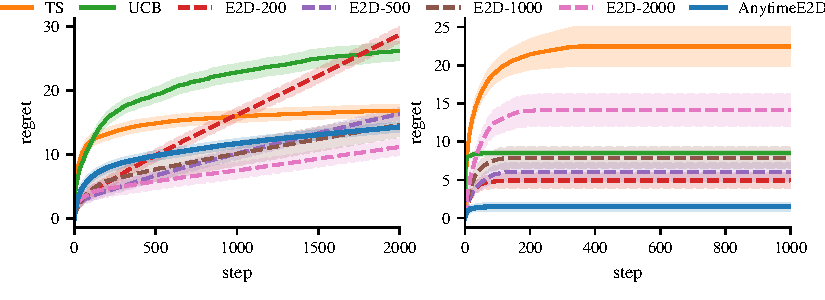
\includegraphics{figures/point-1.pdf}
%     \caption{
%         Running $\AETD$, TS, UCB, and \ETD~optimized for different horizons $n \in \{200, 500, 1000, 2000\}$.
%         Left: The result for horizon $n=2000$, and the feature space dimension $d=3$.
%         Right: The result for horizon $n=1000$, and the feature space dimension $d=30$.
%     }
%     \label{fig:semi-bandit}
% \end{figure}


% \section{Experiment 2}
% In this experiment, we investigate the case when $n < d^4$.
% As pointed out below \cref{lem:p-dec bound}, we expect improvement in this regime as the regret bound of our algorithm is $R_n \leq \min \{d \sqrt{n}, d^{1/3} n^{2/3}\}$, while the default, fixed-horizon \ETD~ algorithm cannot achieve these bounds simultaneously and one has to pick one of $d\sqrt{n}$ or $d^{1/3} n^{2/3}$ beforehand for setting the scale hyperparameter $\lambda$.
% It is standard that the choice of $\lambda$ is made according to the $d \sqrt{n}$ regret bound for \ETD~\cite{foster2021statistical}(which is not optimal when $n <\!\!< d^4$), especially, if the horizon is not known beforehand.
% Thus, we set the horizon to $n=1000$ and the dimension of the feature space to $d=30$, which gives us that $n=1000 <\!\!< 810000 = d^4$.
% The rest of the setup and parameters are the same as in the previous experiment except for the features $\phi_\pi$ and $f^*$ which are again chosen randomly in the beginning and then kept fixed throughout the experiment.

% The results of the experiment can be seen as the right plot in \cref{fig:semi-bandit}.
% As expected, our algorithm \AETD~performs better than \ETD, \UCB, and \TSa.
% This indicates that indeed, \AETD~is likely setting $\lambda$ appropriately to achieve the preferred $d^{1/3}n^{2/3}$ regret rate for small horizons.
% The poor performance of the other algorithms can be justified, since \ETD~is optimized based on the worse $d \sqrt{n}$ regret rate (for small horizons), while the \UCB~and \TSa~algorithms are not known to get regret better than $d \sqrt{n}$.

\renewcommand{\bibname}{References}
\bibliography{ref}
\bibliographystyle{alpha}

\end{document}
